% !Mode:: "TeX:UTF-8"
% Author: Rickjin (ZhihuiJin@gmail.com)
%
\documentclass[fontset=windows,12pt]{ctexrep}
\usepackage{float}
\usepackage{cite}
\usepackage{diagbox}
\usepackage{amsmath}
\usepackage{amsthm}
\usepackage{graphicx}
\usepackage{algorithm}
\usepackage{algorithmic}
\usepackage[colorlinks,bookmarks=false,CJKbookmarks=false,unicode=true,
            linkcolor=blue,anchorcolor=blue,citecolor=green]{hyperref}

%% graphics settings
\graphicspath{{img/}}

%% math settings
\newtheoremstyle{mystyle}{3pt}{3pt}{\songti}{0cm}{\heiti}{}{1em}{}
\theoremstyle{mystyle}

\newtheorem{definition}{\hspace{2em}定义}[section]
\newtheorem{theorem}[definition]{\hspace{2em}定理}
\newtheorem{axiom}[definition]{\hspace{2em}公理}
\newtheorem{lemma}[definition]{\hspace{2em}引理}
\newtheorem{proposition}[definition]{\hspace{2em}命题}
\newtheorem{corollary}[definition]{\hspace{2em}推论}
\newtheorem{remark}{\hspace{2em}注}[section]

\DeclareMathOperator*{\argmax}{arg\,max}
\DeclareMathOperator*{\argmin}{arg\,min}


\begin{document}

% !Mode:: "TeX:UTF-8"
% Author: Rickjin (ZhihuiJin@gmail.com)
%
\hypersetup{CJKbookmarks=true}
\title{\Huge \youyuan \textbf{火光摇曳}}
\author{\youyuan Rickjin(靳志辉) \\
\includegraphics[width=0.3\textwidth]{logo/link-logo.png}
}

\maketitle
\tableofcontents



% !Mode:: "TeX:UTF-8"
% Author: Rickjin (ZhihuiJin@gmail.com)
%
\chapter{正态分布的前世今生}
\label{chap:history-of-normal-distribution}

\begin{verse}
\kaishu{
神说,要有正态分布,就有了正态分布。\\
神看正态分布是好的,就让随机误差服从了正态分布。\\
创世纪---数理统计}
\end{verse}

\section{正态分布,熟悉的陌生人}

学过基础统计学的同学大都对正态分布非常熟悉。这个钟形的分布曲线不但形状优雅,它
对应的密度函数写成数学表达式
$$ \displaystyle f(x)=\frac{1}{\sqrt{2\pi}\sigma}e^{-\frac{{(x-\mu})^2}{2\sigma^2}} $$
也非常具有数学的美感。其标准化后的概率密度函数
$$ \displaystyle f(x)=\frac{1}{\sqrt{2\pi}}e^{-\frac{x^2}{2}} $$
更加的简洁漂亮,两个最重要的数学常量 $\pi$、$e$ 都出现在这公式之中。在我个人的
审美之中,它也属于 top-N 的最美丽的数学公式之一,如果有人问我数理统计领域哪个公
式最能让人感觉到上帝的存在,那我一定投正态分布的票。因为这个分布戴着神秘的面纱
,在自然界中无处不在,让你在纷繁芜杂的数据背后看到隐隐的秩序。

\begin{figure}[H]
\centering
\includegraphics[width=0.8\textwidth]{normal/normal_curve.png}
\caption{正态分布曲线}
\end{figure}

正态分布又通常被称为高斯分布,在科学领域,冠名权那是一个很高的荣誉。2002年以前
去过德国的兄弟们还会发现,德国1991年至2001年间发行的的一款10马克的纸币上印着高
斯(Carl Friedrich Gauss, 1777-1855)的头像和正态密度曲线,而1977年东德发行的20马
克的可流通纪念钢镚上,也印着正态分布曲线和高斯的名字。正态分布被冠名高斯分布,
我们也容易认为是高斯发现了正态分布,其实不然,不过高斯对于正态分布的历史地位的
确立是起到了决定性的作用。

\begin{figure}[htbp]
\centering
\includegraphics[width=0.8\textwidth]{normal/10dm_with_gauss_curve.jpg}
\includegraphics[width=0.4\textwidth]{normal/10dm_with_gauss_curve_detail.jpg}
\includegraphics[width=0.4\textwidth]{normal/20-mark-gauss.jpg}
\caption{德国马克和纪念币上的高斯头像和正态分布曲线}
\end{figure}

正态曲线虽然看上去很美,却不是一拍脑袋就能想到的。我们在本科学习数理统计的时候
,课本一上来介绍正态分布就给出分布密度函数,却从来不说明这个密度函数是通过什么
原理推导出来的。所以我一直搞不明白数学家当年是怎么找到这个概率分布曲线的,又是
怎么发现随机误差服从这个奇妙的分布的。我们在实践中大量的使用正态分布,却对这个
分布的来龙去脉知之甚少,正态分布真是让人感觉既熟悉又陌生。直到我读研究生的时候
,我的导师给我介绍了陈希儒院士的《数理统计学简史》这本书,看了之后才了解了正态
分布曲线从发现到被人们重视进而广泛应用,也是经过了几百年的历史。

正态分布的这段历史是很精彩的,我们通过讲一系列的故事来揭开她的神秘面纱。

\section{邂逅,正态曲线的首次发现}

第一个故事和概率论的发展密切相关,主角是棣莫弗(Abraham de Moivre, 1667-1754) 和
拉普拉斯 (Pierre-Simon Laplace 1749-1827)。拉普拉斯是个大科学家,被称为法国的牛
顿;棣莫弗名气可能不算很大,不过大家应该都应该很熟悉这个名字,因为我们在高中数
学学复数的时候都学过棣莫弗公式 $(\cos\theta + i \sin\theta)^n = \cos(n\theta) +
i \sin(n\theta)$。而棣莫弗所写的《机遇论》(The doctrine of chances)是概率论发
展历史中很重要的一本书。牛顿对棣莫弗十分欣赏,遇到学生向他请教概率方面的问题时,
他就说:“这样的问题应该去找棣莫弗,他对这些问题的研究比我深入得多。”

\begin{figure}[htbp]
\centering
\includegraphics[width=0.25\textwidth]{normal/abraham-de-moivre2.jpg}
\quad \quad
\includegraphics[width=0.25\textwidth]{normal/laplace2.jpg}
\caption{棣莫弗和拉普拉斯}
\end{figure}

古典概率论发源于赌博,惠更斯(Christiaan Huygens, 1629-1695)、帕斯卡(Blaise
Pascal, 1623-1662)、费马(Pierre de Fermat, 1601-1665)、雅可比·贝努利(Jacob
Bernoulli, 1654-1705)都是古典概率的奠基人,他们那会研究的概率问题大都来自赌桌上
,最早的概率论问题是赌徒梅累在1654年向帕斯卡提出的如何分赌金的问题。统计学中的
总体均值之所以被称为期望 (Expectation), 就是源自惠更斯、帕斯卡这些人研究平均情
况下一个赌徒在赌桌上可以期望自己赢得多少钱。

有一天一个哥们,也许是个赌徒,向棣莫弗提了一个和赌博相关的问题:A、B 两人在赌场
里赌博,A、B各自的获胜概率是$p, q=1-p$, 赌 $n$ 局。两人约定:若 A 赢的局数 $X >
np$, 则 A 付给赌场 $X-np$ 元;若 $X<np$,则B 付给赌场 $np-X$ 元。 问赌场挣钱的期
望值是多少。

问题并不复杂, 本质上是一个二项分布,若 $np$ 为整数,棣莫弗求出最后的理论结果是
$$ 2npq b(n, p, np)$$
其中 $ b(n,p,i) = \binom{n}{i}p^iq^{n-i}$ 是常见的二项概率。 但是对具体的 $n$,
因为其中的二项公式中有组合数,要把这个理论结果实际计算出数值结果可不是件容易的
事, 这就驱动棣莫弗寻找近似计算的方法。

与此相关联的另一个问题,是遵从二项分布的随机变量 $ X \sim B(n,p)$, 求X 落在二项
分布中心点一定范围的概率 $ P_d = P(|X - np| \le d)$。

对于 $p=1/2$ 的情形, 棣莫弗做了一些计算并得到了一些近似结果,但是还不够漂亮,
幸运的是棣莫弗和斯特林(James Stirling, 1692-1770)处在同一个时代, 而且二人之间有
联系,斯特林公式是在数学分析中必学的一个重要公式
$$ \displaystyle n! \approx \sqrt{2\pi n} \left(\frac{n}{e}\right)^n .$$

事实上斯特林公式的雏形是棣莫弗最先得到的,但斯特林改进了这个公式,改进的结果为
棣莫弗所用。1733 年,棣莫弗很快利用斯特林公式进行计算并取得了重要的进展。考虑
$n$ 是偶数的情形,二项概率为
$$b(n, \frac{1}{2}, i) = \binom{n}{i}\left(\frac{1}{2}\right)^n$$
以下把$b(n, \frac{1}{2}, i)$简记为$b(i)$, 通过斯特林公式做一些简单的计算容易得到,
$$ \displaystyle b\left(\frac{n}{2}\right) \approx \sqrt{\frac{2}{\pi n}}, $$
$$ \displaystyle \frac{b\left(\frac{n}{2}+d\right)}{b\left(\frac{n}{2}\right)} \approx e^{-\frac{2d^2}{n}}, $$
于是有
$$ \displaystyle b\left(\frac{n}{2}+d\right) \approx \frac{2}{\sqrt{2 \pi n}}e^{-\frac{2d^2}{n}}. $$
使用上式的结果,并在二项概率累加求和的过程中近似的使用定积分代替求和,很容易就
能得到
\begin{eqnarray}
\begin{array}{lll}
\displaystyle P\left(\left|\frac{X}{n} - \frac{1}{2}\right| \le \frac{c}{\sqrt{n}}\right)
& = & \displaystyle \sum_{-c\sqrt{n} \le i \le c\sqrt{n}}b\left(\frac{n}{2}+i\right) \\
& \approx & \displaystyle \sum_{-c\sqrt{n} \le i \le c\sqrt{n}} \frac{2}{\sqrt{2 \pi n}}e^{-\frac{2i^2}{n}}  \\
& = & \displaystyle \sum_{-2c \le \frac{2i}{\sqrt{n}} \le 2c}
\frac{1}{\sqrt{2 \pi}}e^{-\frac{1}{2}(\frac{2i}{\sqrt{n}})^2} \frac{2}{\sqrt{n}} \\
& \approx &\displaystyle  \int_{-2c}^{2c} \frac{1}{\sqrt{2\pi}} e^{-x^2/2} dx .
\end{array}
\end{eqnarray}

看,正态分布的密度函数的形式在积分公式中出现了!这也就是我们在数理统计课本上学
到的一个重要结论:二项分布的极限分布是正态分布。

以上只是讨论了 $p=1/2$ 的情形, 棣莫弗也对 $p \ne 1/2$做了一些计算,后来拉普拉
斯对 $p \ne 1/2$ 的情况做了更多的分析,并把二项分布的正态近似推广到了任意 $p$
的情况。 这是第一次正态密度函数被数学家刻画出来,而且是以二项分布的极限分布的形
式被推导出来的。 熟悉基础概率统计的同学们都知道这个结果其实叫棣莫弗-拉普拉斯中
心极限定理。

\begin{theorem}[棣莫弗-拉普拉斯中心极限定理]
设随机变量 $X_n (n=1,2,\cdots)$ 服从参数为 $n,p$ 的二项分布,则对任意的 $x$, 恒有
$$ \lim_{n\rightarrow\infty}P\left( \frac{X_n - np}{\sqrt{np(1-p)}} \le x \right)
 = \int_{-\infty}^x \frac{1}{\sqrt{2\pi}} e^{\frac{-t^2}{2}}dt .
$$
\end{theorem}

我们在大学学习数理统计的时候,学习的过程都是先学习正态分布,然后才学习中心极限
定理。而学习到正态分布的时候,直接就描述了其概率密度的数学形式,虽然数学上很漂
亮,但是容易困惑数学家们是如何凭空就找到这个分布的。读了陈希孺的《数理统计学简
史》之后,我才明白正态分布的密度形式首次发现是在棣莫弗-拉普拉斯的中心极限定理中
。数学家研究数学问题的进程很少是按照我们数学课本编排的顺序推进的,现代的数学课
本都是按照数学内在的逻辑进行组织编排的,虽然逻辑结构上严谨优美,却把数学问题研
究的历史痕迹抹得一干二净。DNA 双螺旋结构的发现者之一詹姆斯·沃森(James D.
Watson, 1928-) 在他的名著《DNA 双螺旋》序言中说:“ Science seldom proceeds in
the straightforward logical manner imagined by outsiders. (科学的发现很少会像
门外汉所想象的一样,按照直接了当合乎逻辑的方式进行的。)”


棣莫弗给出他的发现后40年(大约是1770年), 拉普拉斯建立了中心极限定理较一般的形
式,中心极限定理随后又被其他数学家们推广到了其它任意分布的情形,而不限于二项分
布。后续的统计学家发现,一系列的重要统计量,在样本量 $N$ 趋于无穷的时候, 其极限
分布都有正态的形式, 这构成了数理统计学中大样本理论的基础。

棣莫弗在二项分布的计算中瞥见了正态曲线的模样,不过他并没有能展现这个曲线的美妙
之处。棣莫弗的这个工作当时并没有引起人们足够的重视,原因在于棣莫弗 不是个统计学
家,从未从统计学的角度去考虑其工作的意义。 正态分布(当时也没有被命名为正态分布)
在当时也只是以极限分布的形式出现,并没有在统计学,尤其是误差分析中发挥作用。这
也就是正态分布最终没有被冠名 棣莫弗分布的重要原因。 那高斯做了啥工作导致统计学
家把正态分布的这顶桂冠戴在了他的头上呢?这先得从最小二乘法的发展说起。

\section{最小二乘法,数据分析的瑞士军刀}

第二个故事的主角是欧拉(Leonhard Euler, 1707-1783)、拉普拉斯、勒让德
(Adrien-Marie Legendre, 1752–1833) 和高斯, 故事发生的时间是18世纪中到19世纪初
。17、18 世纪是科学发展的黄金年代,微积分的发展和牛顿万有引力定律的建立,直接的
推动了天文学和测地学的迅猛发展。当时的大科学家们都在考虑许多天文学上的问题,几
个典型的问题如下:

\begin{enumerate}
\item 土星和木星是太阳系中的大行星,由于相互吸引对各自的运动轨道产生了影响,许
多大数学家,包括欧拉和拉普拉斯都在基于长期积累的天文观测数据计算土星和木星的运
行轨道。

\item 勒让德承担了一个政府给的重要任务,测量通过巴黎的子午线的长度。

\item 海上航行经纬度的定位。主要是通过对恒星和月面上的一些定点的观测来确定经纬度。

\end{enumerate}

这些天文学和测地学的问题,无不涉及到数据的多次测量、分析与计算;17、18世纪的天
文观测,也积累了大量的数据需要进行分析和计算。很多年以前,学者们就已经经验性的
认为,对于有误差的测量数据,多次测量取算术平均是比较好的处理方法。虽然缺乏理论
上的论证,也不断的受到一些人的质疑,取算术平均作为一种异常直观的方式,已经被使
用了千百年, 在多年积累的数据的处理经验中也得到相当程度的验证,被认为是一种良好
的数据处理方法。

以上涉及的问题,我们直接关心的目标量往往无法直接观测,但是一些相关的量是可以观
测到的,而通过建立数学模型,最终可以解出我们关心的量。这些问题都可以用如下数学
模型描述:我们想估计的量是 $\beta_0,\cdots,\beta_p$, 另有若干个可以测量的量
$x_1,\cdots,x_p, y$, 这些量之间有线性关系
$$ y = \beta_0 + \beta_1x_1 + \cdots + \beta_px_p $$
如何通过多组观测数据求解出参数$\beta_0,\cdots,\beta_p$呢? 欧拉和拉普拉斯采用的
的方法都是求解如下线性方程组
\begin{eqnarray}
\left\{
\begin{array}{lll}
 y_1 = \beta_0 + \beta_1x_{11} + \cdots + \beta_px_{p1} \\
 y_2 = \beta_0 + \beta_1x_{12} + \cdots + \beta_px_{p2} \\
\vdots \\
 y_n = \beta_0 + \beta_1x_{1n} + \cdots + \beta_px_{pn} .
\end{array}
\right.
\end{eqnarray}
但是面临的一个问题是,有 $n$ 组观测数据,$p + 1$ 个变量, 如果 $n > p + 1$, 则
得到的线性矛盾方程组,无法直接求解。 所以欧拉和拉普拉斯采用的方法都是通过对数据
的一定的观察,把$n$个线性方程分为 $p+1$组,然后把每个组内的方程线性求和后归并为
一个方程,从而就把$n$个方程的方程组化为$p+1$个方程的方程组,进一步解方程求解
参数。这些方法初看有一些道理,但是都过于经验化, 无法形成统一处理这一类问题的通
用解决框架。

以上求解线性矛盾方程的问题在现在的本科生看来都不困难,这就是统计学中的线性回归
问题,直接用最小二乘法就解决了。可是即便如欧拉、拉普拉斯这些数学大牛,当时也未
能对这些问题提出有效的解决方案。可见在科学研究中,要想在观念上有所突破并不容易
。有效的最小二乘法是勒让德在 1805 年发表的,基本思想就是认为测量中有误差,所以
所有方程的累积误差为
\begin{center}
累积误差 = $\sum($ 观测值 - 理论值 $)^2$
\end{center}
我们求解出导致累积误差最小的参数
\begin{eqnarray}
\label{least-square-error}
\begin{array}{lll}
\hat{\boldsymbol\beta}& = & \displaystyle \argmin_{\boldsymbol {\beta}} \sum_{i=1}^n e_i^2 \\
           & = & \displaystyle
            \argmin_{\boldsymbol\beta} \sum_{i=1}^n\Bigl[y_i - (\beta_0 + \beta_1x_{1i}
            + \cdots + \beta_px_{pi})\Bigr]^2 .
\end{array}
\end{eqnarray}

\begin{figure}[htbp]
\centering
\includegraphics[width=0.3\textwidth]{normal/legendre.jpg}
\caption{勒让德}
\end{figure}

勒让德在论文中对最小二乘法的优良性做了几点说明:
\begin{enumerate}
\item 最小二乘法使得误差平方和最小,并在各个方程的误差之间建立了一种平衡,从而防
      止某一个极端误差取得支配地位;
\item 计算中只要求偏导后求解线性方程组,计算过程明确便捷;
\item 最小二乘法可以导出算术平均值作为估计值。
\end{enumerate}
对于最后一点,推理如下:假设真值为 $\theta$, $x_1, \cdots, x_n$为$n$次测量值, 每
次测量的误差为$ e_i = x_i - \theta $,按最小二乘法,误差累积为
$$ L(\theta) = \sum_{i=1}^n e_i^2 = \sum_{i=1}^n (x_i - \theta)^2 $$
求解$\theta$ 使得 $L(\theta)$达到最小,正好是算术平均 $\overline{x} = \frac{\sum_{i=1}^n x_i}{n} $。

由于算术平均是一个历经考验的方法,而以上的推理说明,算术平均是最小二乘法的一个
特例,所以从另一个角度说明了最小二乘法的优良性,使我们对最小二乘法更加有信心。

最小二乘法发表之后很快得到了大家的认可接受,并迅速的在数据分析实践中被广泛使用
。不过历史上又有人把最小二乘法的发明归功于高斯,这又是怎么一回事呢。高斯在1809
年也发表了最小二乘法,并且声称自己已经使用这个方法多年。高斯发明了小行星定位的
数学方法,并在数据分析中使用最小二乘法进行计算,准确的预测了谷神星的位置。

扯了半天最小二乘法,没看出和正态分布有任何关系啊,离题了吧?单就最小二乘法本身
,虽然很实用,不过看上去更多的算是一个代数方法,虽然可以推导出最优解,对于解的
误差有多大,无法给出有效的分析,而这个就是正态分布粉墨登场发挥作用的地方。勒让
德提出的最小二乘法,确实是一把在数据分析领域披荆斩棘的好刀,但是刀刃还是不够锋
利;而这把刀的打造后来至少一半功劳被归到高斯,是因为高斯不但独自的给出了造刀的
方法,而且把最小二乘这把刀的刀刃磨得无比锋利,把最小二乘法打造成了一把瑞士军刀。
高斯拓展了最小二乘法,把正态分布和最小二乘法联系在一起,并使得正态分布在统计误
差分析中确立了自己的地位,否则正态分布就不会被称为高斯分布了。 那高斯这位神人是
如何把正态分布引入到误差分析之中,打造最小二乘法这把瑞士军刀的呢?

\section{众里寻她千百度,误差分布曲线的确立}

第三个故事有点长,主角是高斯和拉普拉斯,故事的主要内容是寻找随机误差分布的规律。

天文学是第一个被测量误差困扰的学科,从古代至18世纪天文学一直是应用数学最发达的
领域,到18世纪,天文学的发展积累了大量的天文学数据需要分析计算,应该如何来处理
数据中的观测误差成为一个很棘手的问题。我们在数据处理中经常使用平均的常识性法则
,千百来来的数据使用经验说明算术平均能够消除误差,提高精度。算术平均有如此的魅
力,道理何在,之前没有人做过理论上的证明。算术平均的合理性问题在天文学的数据分
析工作中被提出来讨论:测量中的随机误差应该服从怎样的概率分布?算术平均的优良性
和误差的分布有怎样的密切联系?

伽利略在他著名的《关于两个主要世界系统的对话》中,对误差的分布做过一些定性的描
述,主要包括:
\begin{enumerate}
\item 观测数据存在误差
\item 误差是对称分布的;
\item 大的误差出现频率低,小的误差出现频率高。
\end{enumerate}
用数学的语言描述,也就是说误差分布的密度函数 $f(x)$ 关于0对称分布,概率密度随
$|x|$ 增加而减小,这两个定性的描述都很符合常识。

许多天文学家和数学家开始了寻找误差分布曲线的尝试。 天文学家辛普森(Thomas
Simpson, 1710-1761) 先走出了有意义的一步。设真值为 $\theta$, $x_1, \cdots, x_n$
为n次测量值, 每次测量的误差为$ e_i = x_i - \theta $,若用算术平均 $\overline{x} =
\frac{\sum_{i=1}^n x_i}{n} $去估计$\theta$, 其误差为 $\overline{e} =
\frac{\sum_{i=1}^n e_i}{n} $。 辛普森证明了, 对于如下的一个概率分布,

\begin{figure}[ht]
\centering
\includegraphics[width=0.8\textwidth]{normal/simpson-error-curve.jpg}
\caption{辛普森的误差分布曲线}
\end{figure}

有如下结论
$$P(|\overline{e}| < x) \ge P(|e_i|<x) . $$
也就是说,$|\overline{e}|$ 相比于$|e_i|$取小值的机会更大。 辛普森的这个工作很粗糙
,但是这是第一次在一个特定情况下,从概率论的角度严格证明了算术平均的优良性。

从 1772-1774 年, 拉普拉斯也加入到了寻找误差分布密度函数的队伍中。拉普拉斯假定误差
分布密度函数$f(x)$对称且满足
$$ -f'(x) = mf(x) $$
由此可求得分布密度函数为
\begin{equation}
\label{laplace-error-curve}
f(x) = \frac{m}{2} e^{-m|x|} .
\end{equation}
这个概率密度函数现在被称为拉普拉斯分布。

\begin{figure}[ht]
\centering
\includegraphics[width=0.8\textwidth]{normal/laplace-error-curve.jpg}
\caption{拉普拉斯的误差分布曲线}
\end{figure}


以(\ref{laplace-error-curve})式中的函数作为误差分布,拉普拉斯开始考虑如何基于测
量的结果去估计未知参数的值。拉普拉斯可以算是一个贝叶斯主义者,他的参数估计的原
则和现代贝叶斯方法非常相似:假设先验分布是均匀的,计算出参数的后验分布后,取后
验分布的中值点,即$1/2$分位点,作为参数估计值。可是基于这个误差分布密度函数做了
一些计算之后,拉普拉斯发现计算过于复杂,最终没能给出什么有用的结果。

拉普拉斯可是概率论的大牛,写过在概率发展历史中极有影响力的《分析概率论》,不过以我的数学审
美,实在无法理解拉普拉斯这样的牛人怎么找了一个零点不可导的函数作为误差的分布密
度函数,拉普拉斯最终还是没能搞定误差分布的问题。

现在轮到高斯登场了,高斯在数学史中的地位极高,年轻的时候号称数学王子,后来被称
为数学家中的老狐狸,数学家阿贝尔 (Niels Henrik Abel, 1802-1829) 对他的评论是 :
“高斯像一只狐狸,用尾巴将沙地上的足迹抹去(He is like the fox, who effaces his
tracks in the sand with his tail) 。” 我们的数学大师陈省身把黎曼(Georg
Friedrich Bernhard Riemann,1826-1866) 和庞加莱(Jules Henri Poincar\'{e},
1854-1912)称为数学家中的菩萨,而称自己为罗汉;高斯是黎曼的导师,数学圈里有些教
授把高斯称为数学家中的佛。 在数学家中既能仰望理论数学的星空,又能脚踏应用数学的
实地的可不多见,高斯是数学家中少有的顶”天“立”地“的人物,它既对纯理论数学有
深刻的洞察力,又极其重视数学在实践中的应用。 在误差分布的处理中,高斯以极其简单
的手法确立了随机误差的概率分布,其结果成为数理统计发展史上的一块里程碑。

高斯的介入首先要从天文学界的一个事件说起。1801年1月,天文学家朱塞普·皮亚齐
(Giuseppe Piazzi, 1746-1826)发现了一颗从未见过的光度8等的星在移动,这颗现在被称
作谷神星(Ceres)的小行星在夜空中出现6个星期,扫过八度角后就在太阳的光芒下没了
踪影,无法观测。而留下的观测数据有限,难以计算出他的轨道,天文学家也因此无法确
定这颗新星是彗星还是行星,这个问题很快成了学术界关注的焦点。高斯当时已经是很有
名望的年轻数学家了,这个问题引起了他的兴趣。高斯以其卓越的数学才能创立了一种崭
新的行星轨道的计算方法,一个小时之内就计算出了谷神星的轨道,并预言了他在夜空中
出现的时间和位置。 1801年12月31 日夜,德国天文爱好者奥伯斯(Heinrich Olbers,
1758-1840),在高斯预言的时间里,用望远镜对准了这片天空。果然不出所料,谷神星出
现了!

高斯为此名声大震,但是高斯当时拒绝透露计算轨道的方法,原因可能是高斯认为自己的
方法的理论基础还不够成熟,而高斯一向治学严谨、精益求精,不轻易发表没有思考成熟
的理论。直到1809年高斯系统地完善了相关的数学理论后,才将他的方法公布于众,而其
中使用的数据分析方法,就是以正态误差分布为基础的最小二乘法。那高斯是如何推导出
误差分布为正态分布的?让我们看看高斯是如何猜测上帝的意图的。

设真值为 $\theta$, $x_1, \cdots, x_n$为$n$次独立测量值, 每次测量的误差为$ e_i = x_i - \theta $,
假设误差$e_i$的密度函数为 $f(e)$, 则测量值的联合概率为$n$个误差的联合概率,记为
\begin{align*}
L(\theta) & = L(\theta;x_1,\cdots,x_n)=f(e_1)\cdots f(e_n) \\
& = f(x_1-\theta)\cdots f(x_n-\theta)
\end{align*}
但是高斯不采用贝叶斯的推理方式,而是直接取使$L(\theta)$达到最大值的
$\hat{\theta}=\hat{\theta}(x_1,\cdots,x_n)$ 作为$\theta$的估计值,即
$$ \hat{\theta}= \argmax_{\theta} L(\theta) .$$
现在我们把$L(\theta)$ 称为样本的似然函数,而得到的估计值$ \hat{\theta}$ 称为极
大似然估计。高斯首次给出了极大似然的思想,这个思想后来被统计学家费希尔系统的发
展成为参数估计中的极大似然估计理论。

数学家波利亚(George P\'{o}lya, 1887-1985)说过:“要成为一个好的数学家,……,你必须
首先是一个好的猜想家(To be a good mathematician,..., you must be a good
guesser)。”历史上一流的数学家都是伟大的猜想家。高斯接下来的想法特别牛,他开始
揣度上帝的意图,而这充分体现了高斯的数学天才。高斯把整个问题的思考模式倒过来:
既然千百年来大家都认为算术平均是一个好的估计,那我就认为极大似然估计导出的就应
该是算术平均!所以高斯猜测上帝在创世纪中的旨意就是:
\begin{center}
\bf{误差分布导出的极大似然估计 = 算术平均值}
\end{center}

然后高斯去找误差密度函数 $f$ 以迎合这一点。即寻找这样的概率分布密度函数 $f$, 使
得极大似然估计正好是算术平均 $\hat{\theta} = \overline{x}$。而高斯应用数学技巧求解这
个函数$f$, 高斯证明(证明不难,后续给出),所有的概率密度函数中,唯一满足这个性质
的就是 $$ \displaystyle
f(x)=\frac{1}{\sqrt{2\pi}\sigma}e^{-\frac{x^2}{2\sigma^2}} $$ 瞧,正态分布的密
度函数 $N(0, \sigma^2)$ 被高斯他老人家给解出来了!

进一步,高斯基于这个误差分布的密度函数对最小二乘法给出了一个很漂亮的解释。对于
最小二乘公式中涉及的每个误差 $e_i$(见上文公式(\ref{least-square-error})), 由于
误差服从概率分布 $N(0, \sigma^2)$, 则$(e_1, \cdots, e_n)$ 的概率为
$$\frac{1}{(\sqrt{2\pi}\sigma)^n}\exp\left\{-\frac{1}{2\sigma^2} \sum_{i=1}^n e_i^2 \right\} .$$
要使得这个概率最大,必须使得$\sum_{i=1}^n e_i^2 $ 取最小值,这正好就是最小二
乘法的要求。

高斯所拓展的最小二乘法成为了19世纪统计学的最重要成就,它在19世纪统计学的重要性
就相当于18世纪的微积分之于数学。而勒让德和高斯的关于最小二乘法的发明权之争,成
了数学史上仅次于牛顿、莱布尼茨微积分发明权的争端。相比于勒让德1805年给出的最小
二乘法描述,高斯基于误差正态分布的最小二乘理论显然更高一筹,高斯的工作中既提出
了极大似然估计的思想,又解决了误差的概率密度分布的问题,由此我们可以对误差大小
的影响进行统计度量了。高斯的这项工作对后世的影响极大,而正态分布也因此被冠名高
斯分布。估计高斯本人当时是完全没有意识到他的这个工作给现代数理统计学带来的深刻
影响。高斯在数学上的贡献特多,去世前他是要求给自己的墓碑上雕刻上正十七边形,以
说明他在正十七边形尺规作图上的杰出工作。而后世的德国钞票和钢镚上是以正态密度曲
线来纪念高斯,这足以说明高斯的这项工作在当代科学发展中的分量。

17、18世纪科学界流行的做法,是尽可能从某种简单明了的准则(first principle)出
发进行逻辑推导。高斯设定了准则“最大似然估计应该导出优良的算术平均”,并导出了
误差服从正态分布,推导的形式上非常简洁优美。但是高斯给的准则在逻辑上并不足以让
人完全信服,因为算术平均的优良性当时更多的是一个经验直觉,缺乏严格的理论支持。
高斯的推导存在循环论证的味道:因为算术平均是优良的,推出误差必须服从正态分布;
反过来,又基于正态分布推导出最小二乘法和算术平均,来说明最小二乘法和算术平均的优
良性。这陷入了一个鸡生蛋蛋生鸡的怪圈,逻辑上算术平均的优良性到底有没有自行成立
的理由呢?

高斯的文章发表之后,拉普拉斯很快得知了高斯的工作。拉普拉斯看到,正态分布既可以
从抛钢镚产生的序列和中生成出来,又可以被优雅的作为误差分布定律,这难道是偶然现
象?拉普拉斯不愧为概率论的大牛,他马上将误差的正态分布理论和中心极限定理联系起
来,提出了元误差解释。他指出如果误差可以看成许多微小量的叠加,则根据他的中心极
限定理,随机误差理所应当是高斯分布。而20世纪中心极限定理的进一步发展,也给这个
解释提供了更多的理论支持。因此以这个解释为出发点,高斯的循环论证的圈子就可以
打破。 估计拉普拉斯悟出这个结论之后一定想撞墙,自己辛辛苦苦寻寻觅觅了这么久的误
差分布曲线就在自己的眼皮底下,自己却长年视而不见,被高斯占了先机。

至此,误差分布曲线的寻找尘埃落定,正态分布在误差分析中确立了自己的地位,并在整
个19世纪不断的开疆扩土,直至在统计学中鹤立鸡群,傲世其它一切概率分布;而高斯和
拉普拉斯的工作,为现代统计学的发展开启了一扇大门。

在整个正态分布被发现与应用的历史中,棣莫弗、拉普拉斯、高斯各有贡献,拉普拉斯从
中心极限定理的角度解释它,高斯把它应用在误差分析中,殊途同归。正态分布被人们发
现有这么好的性质,各国人民都争抢它的冠名权。因为拉普拉斯是法国人,所以当时在法
国被称为拉普拉斯分布;而高斯是德国人, 所以在德国叫做高斯分布;第三中立国的人民
称他为拉普拉斯-高斯分布。后来法国的大数学家庞加莱建议改用正态分布这一中立名称,
而随后统计学家卡尔·皮尔森使得这个名称被广泛接受:

\begin{quotation}
\emph{Many years ago I called the Laplace-Gaussian curve the normal curve,
which name, while it avoids an international question of priority,
has the disadvantage of leading people to believe that all other distributions
of frequency are in one sense or another "abnormal".}

\emph{ ---Karl Pearson (1920) }
\end{quotation}

不过因为高斯在数学家中的名气实在是太大, 正态分布的桂冠还是更多地被戴在了高斯的脑
门上,目前数学界通行的用语是正态分布、高斯分布, 两者并用。

正态分布在高斯的推动下,迅速在测量误差分析中被广泛使用,然而早期也仅限于测量误
差的分析中,其重要性远没有被自然科学和社会科学领域中的学者们所认识,那正态分布
是如何从测量误差分析的小溪,冲向自然科学和社会科学的汪洋大海的呢?

\section{曲径通幽处,禅房花木深}

在介绍正态分布的后续发展之前,我们来多讲一点数学,也许有些人会觉得枯燥,不过高
斯曾经说过:“数学是上帝的语言”;所以要想更加深入的理解正态分布的美,唯有借助
于上帝的语言。

造物主造物的准则往往是简单明了的,只是在纷繁芜杂的万物之中,我们要发现并领会它
并非易事。之前提到过,17、18世纪科学界流行的做法,是尽可能从某种简单明了的准则
出发作为科学探求的起点;而后来的数学家和物理学家们的研究发现,屡次从一些给定的
简单的准则出发, 我们总是被引领到了正态分布的家门口,这让人感觉到正态分布的美妙。

达尔文的表弟高尔顿是生物学家兼统计学家,他对正态分布非常的推崇与赞美:”我几乎
不曾见过像误差呈正态分布这么激发人们无穷想象的宇宙秩序“。当代两位伟大的概率学
家列维(Paul Pierre L\'{e}vy, 1886-1971) 和卡克(Mark Kac, 1914-1984) 都曾经说过,
正态分布是他们切入概率论的初恋情人,具有无穷的魅力。如果古希腊人知道正态分布,
想必奥林匹斯山的神殿里会多出一个正态女神,由她来掌管世间的混沌。

要拉下正态分布的神秘面纱展现她的美丽,需要高深的概率论知识,本人在数学方面知识
浅薄,不能胜任。只能在极为有限的范围内尝试掀开她的面纱的一角。棣莫弗和拉普拉斯
以抛钢镚的序列求和为出发点,沿着一条小径第一次把我们领到了正态分布的家门口,这
条路叫做中心极限定理。而这条路上风景秀丽,许多概率学家都为之倾倒。这条路在二十
世纪被概率学家们越拓越宽,成为了通往正态曲线的一条康庄大道。而数学家和物理学家
们发现:条条小路通正态。著名的物理学家杰恩斯(Edwin Thompson Jaynes, 1922-1998)
在他的名著《概率论沉思录(Probability Theory: the Logic of Science)》中,描绘了
四条通往正态分布的小径;曲径通幽处,禅房花木深,让我们一起来欣赏一下这四条小径
上的风景吧。

\subsection{高斯(1809)的推导}

第一条小径是高斯找到的,高斯以如下准则作为小径的出发点
\begin{center}
误差分布导出的极大似然估计 = 算术平均值
\end{center}

设真值为 $\theta$, $x_1, \cdots, x_n$为n次独立测量值, 每次测量的误差为$ e_i =
x_i - \theta $,假设误差$e_i$的密度函数为 $f(e)$, 则测量值的联合概率为$n$个误差的联
合概率,记为
\begin{align*}
L(\theta) &= L(\theta;x_1,\cdots,x_n)=f(e_1)\cdots f(e_n)  \\
& = f(x_1-\theta)\cdots f(x_n-\theta)
\end{align*}
为求极大似然估计,令
$$\frac{d \log L(\theta)}{d \theta} = 0$$
整理后可以得到
$$ \sum_{i=1}^n \frac{f'(x_i-\theta)}{f(x_i-\theta)} = 0 $$
令 $g(x) = \frac{f'(x)}{f(x)}$,
$$ \sum_{i=1}^n g(x_i-\theta) = 0 $$
由于高斯假设极大似然估计的解就是算术平均 $\bar{x}$,把解代入上式,可以得到
\begin{equation}
\label{gauss-derivation}
\sum_{i=1}^n g(x_i-\bar{x}) = 0
\end{equation}
(\ref{gauss-derivation})式中取 $n=2$, 有
$$g(x_1-\bar{x}) + g(x_2-\bar{x}) = 0$$
由于此时有 $ x_1-\bar{x} = -(x_2-\bar{x})$, 并且 $x_1, x_2$ 是任意的,由此得到
$$ g(-x) = -g(x) $$
(\ref{gauss-derivation})式中再取 $n=m+1$, 并且要求 $x_1=\cdots=x_m=-x, x_{m+1} =
mx$, 则有 $\bar{x} = 0$, 并且
$$ \sum_{i=1}^n g(x_i-\bar{x}) = mg(-x) + g(mx) $$
所以得到
$$g(mx) = mg(x)$$
而满足上式的唯一的连续函数就是 $g(x)=cx$, 从而进一步可以求解出
$$f(x) = Me^{cx^2}$$
由于$f(x)$是概率密度函数,把$f(x)$ 正规化一下就得到均值为$0$的正态分布密度函数
$N(0,\sigma^2)$。

\subsection{赫歇尔(1850)和麦克斯韦(1860) 的推导}

第二条小径是天文学家赫歇尔(John Frederick William Herschel, 1792-1871)和物理学
家麦克斯韦(James Clerk Maxwell, 1831-1879) 发现的。 1850年,天文学家赫歇尔在对星
星的位置进行测量的时候,需要考虑二维的误差分布,为了推导这个误差的概率密度分布
$p(x,y)$,赫歇尔设置了两个准则:
\begin{enumerate}
\item $x$ 轴和 $y$ 轴的误差是相互独立的,即随机误差在正交的方向上相互独立
\item 误差的概率分布在空间上具有旋转对称性,即误差的概率分布和角度没有关系
\end{enumerate}
这两个准则对于赫歇尔考虑的实际测量问题看起来都很合理。由第一条准则,可以得到
$p(x,y)$ 应该具有如下形式
$$ p(x,y) = f(x) * f(y) $$
把这个函数转换为极坐标,在极坐标下的概率密度函数设为 $g(r,\theta)$, 有
$$ p(x,y) =  p(rcos\theta, rsin\theta) = g(r,\theta)$$
由第二条准则, $g(r,\theta)$ 具有旋转对称性,也就是应该和 $\theta$ 无关, 所以 $g(r,\theta)=g(r)$,
综上所述,我们可以得到
$$ f(x)f(y) = g(r) = g(\sqrt{x^2+y^2}) $$
取 $y=0$, 得到 $g(x) = f(x)f(0)$, 所以上式可以转换为
$$ \log\left[\frac{f(x)}{f(0)}\right] + \log\left[\frac{f(y)}{f(0)}\right]
= \log\left[\frac{f(\sqrt{x^2+y^2})}{f(0)}\right] $$
令 $\log\left[\frac{f(x)}{f(0)}\right] = h(x) $, 则有
$$ h(x) + h(y) = h(\sqrt{x^2+y^2}) $$
从这个函数方程中可以解出 $h(x) = ax^2$, 从而可以得到 $f(x)$ 的一般形式如下
$$ f(x) = \sqrt{\frac{\alpha}{\pi}} e^{-\alpha x^2} $$
而 $f(x)$ 就是正态分布 $N(0, 1/\sqrt{2\alpha)}$, 从而 $p(x,y)$ 就是标准二维正态
分布的密度函数
$$ p(x,y) = \frac{\alpha}{\pi} e^{-\alpha (x^2+y^2)}. $$

1860 年,伟大的物理学家麦克斯韦在考虑气体分子的运动速度分布的时候,在三维空
间中基于类似的准则推导出了气体分子运动的分布是正态分布
$\rho(v_x,v_y,v_z) \propto \exp\{-\alpha(v_x^2+v_y^2+v_z^2)\} $。这就是著名的麦
克斯韦分子速率分布定律。大家还记得我们在普通物理中学过的麦克斯韦-波尔兹曼气体速
率分布定律吗?
\begin{eqnarray}
\label{maxwell}
\begin{array}{lll}
F(v) & = & \displaystyle \left(\frac{m}{2\pi kT}\right)^{3/2} e^{-\frac{mv^2}{2kT}} \\
& = & \displaystyle  \left(\frac{m}{2\pi kT}\right)^{1/2} e^{-\frac{mv_x^2}{2kT}}
                     \times \left(\frac{m}{2\pi kT}\right)^{1/2} e^{-\frac{mv_y^2}{2kT}}
                     \times \left(\frac{m}{2\pi kT}\right)^{1/2} e^{-\frac{mv_z^2}{2kT}} .
\end{array}
\end{eqnarray}
所以这个分布其实是三个正态分布的乘积, 你的物理老师是否告诉过你其实这个分布就是
三维正态分布?

赫歇尔-麦克斯韦推导的神妙之处在于,没有利用任何概率论的知识,只是基于空间几何的
不变性,就推导出了正态分布。美国诺贝尔奖物理学家费曼(Richard Feymann,1918-1988)
每次看到一个有 $\pi$的数学公式的时候,就会问:圆在哪里?这个推导中使用到了
$x^2+y^2$, 也就是告诉我们正态分布密度公式中有个$\pi$, 其根源在于二维正态分布中
的等高线恰好是个圆。

\subsection{兰登(1941)的推导}

第三条道是一位电气工程师兰登(Vernon D. Landon)给出的。1941 年, 兰登研究通信电
路中的噪声电压,通过分析经验数据他发现噪声电压的分布模式很相似,不同的是分布的
层级,而这个层级可以使用方差 $\sigma^2$ 来刻画。因此他推理认为噪声电压的分布密度函
数形式是 $p(x;\sigma^2)$。假设原来的电压为X, 累加了一个相对其方差 $\sigma$而言
很微小的误差扰动 $\epsilon$, $\epsilon$ 的概率密度是 $q(e)$, 那么新的噪声电压
是 $X' = X + \epsilon$。 兰登提出了如下的准则

\begin{enumerate}
\item 随机噪声具有稳定的分布模式
\item 累加一个微小的随机噪声,不改变其稳定的分布模式,只改变分布的层级(用方差度量)
\end{enumerate}
用数学的语言描述: 如果 $$X \sim p(x;\sigma^2), \epsilon \sim q(e), X'= X+\epsilon$$
则有 $$X' \sim p(x;\sigma^2 + var(\epsilon))$$

现在我们来推导函数$p(x;\sigma^2)$ 应该长成啥样。按照两个随机变量和的分布的计算
方式, $X'$ 的分布密度函数将是 $X$ 的分布密度函数和 $\epsilon$的分布密度函数的
卷积,即有
$$ f(x') = \int p(x'-e; \sigma^2)q(e)de $$
把 $p(x'-e; \sigma^2)$ 在$x'$处做泰勒级数展开(为了方便,展开后把自变量由 $x'$
替换为 $x$), 上式可以展开为
$$ f(x) = p(x; \sigma^2) - \frac{\partial p(x; \sigma^2)}{\partial x} \int eq(e)de +
\frac{1}{2} \frac{\partial^2 p(x; \sigma^2)}{\partial x^2} \int e^2q(e)de + \cdots
$$
将$p(x; \sigma^2)$简记为$p$,则有
$$ f(x) = p - \frac{\partial p}{\partial x} \overline{\epsilon} +
\frac{1}{2} \frac{\partial^2 p}{\partial x^2}\overline{\epsilon^2} + o(\overline{\epsilon^2})
$$

对于微小的随机扰动 $\epsilon$, 我们认为他取正值或者负值是对称的,所以
$\overline{\epsilon} = 0 $。所以有
\begin{equation}
\label{landon-x}
 f(x) = p + \frac{1}{2} \frac{\partial^2 p}{\partial x^2}\overline{\epsilon^2} + o(\overline{\epsilon^2})
\end{equation}

对于新的噪声电压 $X' = X + \epsilon$, 方差由$\sigma^2$ 增加为 $\sigma^2 + var(\epsilon) =
\sigma^2 + \overline{\epsilon^2}$,所以按照兰登的分布密度函数模式不变的假设, 新的
噪声电压的分布密度函数应该为 $f(x) = p(x; \sigma^2 +  \overline{\epsilon^2})$。把$p(x;
\sigma^2 +  \overline{\epsilon^2})$ 在 $\sigma^2$ 处做泰勒级数展开,得到
\begin{equation}
\label{landon-sigma}
f(x) = p + \frac{\partial p}{\partial \sigma^2}\overline{\epsilon^2} + o(\overline{\epsilon^2})
\end{equation}
比较 (\ref{landon-x}) 和 (\ref{landon-sigma}) 这两个式子,可以得到如下偏微分方程
$$ \frac{1}{2} \frac{\partial^2 p}{\partial x^2} = \frac{\partial p}{\partial \sigma^2} $$
而这个方程就是物理上著名的扩散方程(diffusion equation),求解该方程就得到
$$ p(x; \sigma^2) = \frac{1}{\sqrt{2\pi}\sigma}e^{-\frac{x^2}{2\sigma^2}} $$
又一次,我们推导出了正态分布!

杰恩斯对于这个推导的评价很高,认为兰登 的推导本质上给出了自然界的噪音形
成过程。他指出这个推导这基本上就是中心极限定理的增量式版本,相比于中心极限定
理是一次性累加所有的因素,兰登 的推导是每次在原有的分布上去累加一个微小的扰动
。而在这个推导中,我们看到,正态分布具有相当好的稳定性;只要数据中正态的模式已
经形成,他就容易继续保持正态分布,无论外部累加的随机噪声 $q(e)$ 是什么分布,正
态分布就像一个黑洞一样把这个累加噪声吃掉。

\subsection{基于最大熵的推导}

还有一条小径是基于最大熵原理的, 物理学家杰恩斯在最大熵原理上有非常重要的
贡献,他在《概率论沉思录》里面对这个方法有描述和证明,没有提到发现者,我不确认
这条道的发现者是否是杰恩斯本人。

熵在物理学中由来已久,信息论的创始人香农(Claude Elwood Shannon, 1916-2001)把这个
概念引入了信息论,学习机器学习的同学们都知道目前机器学习中有一个非常好用的分类
算法叫最大熵分类器。要想把熵和最大熵的来龙去脉说清楚可不容易,不过这条道的风景
是相当独特的,杰恩斯对这条道也是偏爱有加。

对于一个概率分布 $p(x)$, 我们定义他的熵为
$$H(p) = -\int p(x)\log p(x) dx$$

如果给定一个分布密度函数 $p(x)$ 的均值 $\mu$ 和方差 $\sigma^2$(给定均值和方差这个条
件,也可以描述为给定一阶原点矩和二阶原点矩,这两个条件是等价的), 则在所有满足
这两个限制的概率分布中,熵最大的概率分布 $p(x|\mu, \sigma^2)$ 就是正态分布
$N(\mu, \sigma^2)$。

这个结论的推导数学上稍微有点复杂,不过如果已经猜到了给定限制条件下最大熵的分布
是正态分布,要证明这个猜测却是很简单的,证明的思路如下。

考虑两个概率分布 $p(x)$和$q(x)$,使用不等式 $\log x \le (x-1) $, 得
$$ \int p(x) \log \frac{q(x)}{p(x)} dx \le \int p(x) (\frac{q(x)}{p(x)} - 1) dx
= \int q(x) dx - \int p(x) dx = 0 $$
于是
$$ \int p(x) \log \frac{q(x)}{p(x)} dx = \int p(x) \log\frac{1}{p(x)}dx + \int p(x) \log q(x) dx \le 0 $$
所以
\begin{equation}
 H(p) \le -\int p(x) \log q(x) dx
\end{equation}
熟悉信息论的同学都知道,这个式子是信息论中的很著名的结论:一个概率分布的熵总是
小于交叉熵。上式要取等号当且仅当$q(x)=p(x)$。

对于 $p(x)$, 在给定的均值 $\mu$ 和方差 $\sigma^2$下, 我们取$q(x)=N(\mu,
\sigma^2)$, 则可以得到
\begin{eqnarray}
\begin{array}{lll}
 H(p) &  \le &\displaystyle - \int p(x) \log \left\{ \frac{1}{\sqrt{2\pi}\sigma}
 e^{-\frac{{(x-\mu})^2}{2\sigma^2}}\right\} dx \\
 & = & \displaystyle \int p(x) \left\{ \frac{(x-\mu)^2}{2\sigma^2}  + \log \sqrt{2\pi}\sigma \right\} dx \\
 & = & \displaystyle \frac{1}{2\sigma^2} \int p(x)(x-\mu)^2 dx + \log \sqrt{2\pi}\sigma
\end{array}
\end{eqnarray}
由于 $p(x)$ 的均值方差有如下限制
$$ \int p(x) (x-\mu)^2 dx = \sigma^2$$
于是
$$  H(p) \le \frac{1}{2\sigma^2}\sigma^2 + \log \sqrt{2\pi}\sigma  =  \frac{1}{2} + \log \sqrt{2\pi}\sigma $$
而当$p(x)=N(\mu, \sigma^2)$的时候,上式可以取到等号,这就证明了结论。


杰恩斯显然对正态分布具有这样的性质极为赞赏,因为这从信息论的角度证明了正态
分布的优良性。而我们可以看到,正态分布熵的大小,取决于方差的大小。 这也容易理解
, 因为正态分布的均值和密度函数的形状无关,正态分布的形状是由其方差决定的,而熵
的大小反应概率分布中的信息量,显然和密度函数的形状相关。

好的,风景欣赏暂时告一段落。所谓“横看成岭侧成峰,远近高低各不同”,正态分布给
人们提供了多种欣赏角度和想象空间。法国菩萨级别的大数学家庞加莱对正态分布说过一
段有意思的话,引用来作为这个小节的结束:
\begin{quotation}
\emph{
Physicists believe that the Gaussian law has been proved in mathematics
while mathematicians think that it was experimentally established in physics. }
\kaishu{(物理学家认为高斯分布已经在数学上得到证明,而数学家则认为高斯分布在物理试验中得
到确认。) }
\\
\emph{--- Henri Poincar\'{e}}
\end{quotation}

\section{开疆拓土,正态分布的进一步发展}

19世纪初,随着拉普拉斯中心极限定理的建立与高斯正态误差理论的问世,正态分布开始
崭露头角,逐步在近代概率论和数理统计学中大放异彩。在概率论中,由于拉普拉斯的推
动,中心极限定理发展成为现代概率论的一块基石;而在数理统计学中,在高斯的大力提
倡之下,正态分布开始逐步畅行于天下。

\subsection{论剑中心极限定理}

先来说说正态分布在概率论中的地位,这个主要是由于中心极限定理的影响。 1776 年,
拉普拉斯开始考虑一个天文学中的彗星轨道的倾角的计算问题,最终的问题涉及独立随机
变量求和的概率计算,也就是计算如下的概率值
$$ S_n = X_1 + X_2 + \cdots + X_n  $$
$$P(a < S_n < b) = ? $$

在这个问题的处理上,拉普拉斯充分展示了其深厚的数学分析功底和高超的概率计算技巧
,他首次引入了特征函数(也就是对概率密度函数做傅立叶变换)来处理概率分布的神妙方
法,而这一方法经过几代概率学家的发展,在现代概率论里面占有极其重要的位置。基于
这一分析方法,拉普拉斯通过近似计算,在他1812年发表的名著《分析概率论》中给
出了中心极限定理的一般描述:

\begin{theorem}[拉普拉斯, 1812] $ e_i (i=1, \cdots n)$ 为独立同分布的测量误差,
具有均值$\mu$ 和方差 $\sigma^2$,如果 $\lambda_1, \cdots, \lambda_2$ 为常数,
$a>0$, 则有
$$ \displaystyle P\left(\left|\sum_{i=1}^n \lambda_i(e_i - \mu)\right|
\le a \sqrt{\sum_{i=1}^n \lambda_i^2}\right)
\approx \frac{2}{\sqrt{2\pi}\sigma} \int_0^a e^{-\frac{x^2}{2\sigma^2}} dx . $$
\end{theorem}

这已经是比棣莫弗-拉普拉斯中心极限定理更加深刻的一个结论了,理科专业的本科生学习
《概率论与数理统计》这门课程的时候,通常学习的中心极限定理的一般形式如下:

\begin{theorem}[林德伯格-列维 中心极限定理]
设$X_1,\cdots, X_n$ 独立同分布,且具有有限的均值 $\mu$ 和方差 $\sigma^2$ ,
则在 $n \rightarrow \infty$ 时,有
$$ \displaystyle \frac{\sqrt{n}(\overline{X} - \mu)}{\sigma}  \rightarrow  N(0,1) .$$
\end{theorem}

多么奇妙的性质,随意的一个概率分布中生成的随机变量,在序列和(或者等价的求算术平
均)的操作之下,表现出如此一致的行为,统一的规约到正态分布。

\begin{figure}[bp]
\centering
\vspace{1cm}
\includegraphics[width=0.7\textwidth]{normal/central_limit_theorem.eps}
\caption{中心极限定理}
\end{figure}

概率学家们进一步的研究结果更加令人惊讶,序列求和最终要导出正态分布的条件并不需
要这么苛刻,即便 $X_1,\cdots, X_n$ 并不独立,也不具有相同的概率分布形式,很多时
候他们求和的最终归宿仍然是正态分布。一切的纷繁芜杂都在神秘的正态曲线下被消解
,这不禁令人浮想联翩。中心极限定理恐怕是概率论中最具有宗教神秘色彩的定理,如果
有一位牧师拿着一本圣经向我证明上帝的存在,我是丝毫不会买账;可是如果他向我展示
中心极限定理并且声称那是神迹,我可能会有点犹豫,从而乐意倾听他的布道。如果我能
坐着时光机穿越到一个原始部落中,我也一定带上中心极限定理,并劝说部落的酋长把正
态分布作为他们的图腾。

中心极限定理虽然表述形式简洁,但是严格证明它却非常困难。中心极限定理就像一张大
蜘蛛网,棣莫弗和拉普拉斯编织了它的雏形,可是这张网上漏洞太多,一个多世纪来,数
学家们就像蜘蛛一样前赴后继,努力想把所有的漏洞都补上。在19世纪,泊松
(Sim\'{e}on Denis Poisson, 1781-1840)、狄利克莱(Gustav Lejeune Dirichlet,
1805-1859)、柯西(Augustin-Louis Cauchy, 1789-1857)、贝塞尔(Friedrich Bessel,
1784-1846)这些大蜘蛛都曾经试图对把这张网上的漏洞补上。从现代概率论的角度来看,
整个19世纪的经典概率理论并没有能输出一个一般意义下的严格证明。而最终把漏洞补上
的是来自俄罗斯的几位蜘蛛侠:切比雪夫(Pafnuty Chebyshev, 1821-1894)、马尔可夫(Andrey Andreyevich Markov,
1856-1922)和李雅普诺夫(Aleksandr Mikhailovich Lyapunov, 1857-1918)。

俄罗斯是一个具有优秀数学传统的民族,产生过几位顶尖的的数学家,在现代概率论的发展中,俄
罗斯的圣彼得堡学派可以算是顶了大半边天,而切比雪夫正是圣彼得堡数学学派的奠基人和领袖。
把中心极限定理证明中的漏洞补上的方案的雏形是从切比雪夫
1887年的工作开始的,切比雪夫提出了一个基于矩法的证明,矩法是概率分析中比较传统的方法,
使用的数学工具比较基础,不过切比雪夫这个证明也还存在一些漏洞。马尔可夫和李雅普诺夫都是切
比雪夫的学生,两人在中心极限定理的严格证明上展开了竞赛。马尔科夫在概率论里面可算是大名鼎鼎,
马尔科夫链是应用最为广泛的概率模型之一。马尔科夫和他的老师切比雪夫一样,他们在数学中的
研究风格都偏向于使用初等、简单易懂的数学工具来证明复杂艰深的定理。
马尔科夫沿着老师的基于矩法的思路在蜘蛛网上辛勤编织,在证明上做了很多的修补,但洞还是补得
不够严实。李雅普诺夫不像马尔可夫那样深受老师的影响,他沿着拉普拉斯当年提出的基
于特征函数的思路,于1901年给出了一个补洞的方法,切比雪夫对这个方法大加赞赏,李
雅普诺夫的证明被认为是第一个在一般条件下的严格证明;而马尔科夫也不甘示弱,在
1913年基于矩法也把洞给补严实了。

\begin{figure}[htbp]
\centering
\includegraphics[width=1.0\textwidth]{normal/clt_proof.jpg}
\caption{华山论剑}
\end{figure}

20世纪初期到中期,中心极限定理的研究几乎吸引了所有的概率学家,这个定理俨然成为
了概率论的明珠,成为了各大概率论武林高手华山论剑的场所。不知道大家对中心极限定
理中的“中心”一词如何理解,许多人都认为“中心”这个词描述的是这个定理的行为:以
正态分布为中心。这个解释看起来确实合情合理,不过并不符合该定理被冠名的历史。事
实上,20世纪初概率学家大都称呼该定理为极限定理(Limit Theorem),由于该定理在概率
论中处于如此重要的中心位置,如此之多的概率学武林高手为它魂牵梦绕,于是数学家波
利亚于1920年在该定理前面冠以“中心”一词,由此后续人们都称之为中心极限定理。

数学家们总是极其严谨苛刻的,给定了一个条件下严格证明了中心极限定理,数学家们就开
始探寻中心极限定理成立的各种条件,询问这个条件是否充分必要条件,并且进一步追问
序列和在该条件下以什么样的速度收敛到正态分布。1922年林德伯格(Jarl Waldemar
Lindeberg, 1876-1932) 基于一个比较宽泛容易满足的条件,为中心极限定理提出了一个很
容易理解的初等证明,这个条件我们现在称之为林德伯格条件。然后概率学家费勒
(William Feller, 1906-1970) 和列维就开始追问:林德伯格条件是充分必要的吗?基于林
德伯格的工作, 费勒和列维都于 1935 年独立的得到了中心极限定理成立的充分必要条件
,这个条件可以用直观的非数学语言描述如下:

\begin{theorem}[中心极限定理充要条件]
假设独立随机变量序列 $X_i$ 的中值为0, 要使序列和 $\displaystyle S=\sum_{i=1}^n
X_i$ 的分布密度函数逼近正态分布,以下条件是充分必要的:
\begin{enumerate}
\item 如果 $X_i$相对于序列和$S$的散布(可以理解为标准差)是不可忽略的,则 $X_i$ 的分
      布必须接近正态分布;
\item 对于所有可忽略的 $X_i$, 取绝对值最大的那一项,这个绝对值相对于序列和
      也是可忽略的。
\end{enumerate}
\end{theorem}

事实上这个充分必要条件发现的优先权,费勒和列维之间还着实出现了一些争论,当然他
们俩都是独立的几乎在同一时间解决了这个问题。在列维证明这个充分必要条件的过程中
,列维发现了正态分布的一个有趣的性质。我们在数理统计中都学过,如果两个独立随机
变量 $X,Y$ 具有正态分布,则$S=X+Y$ 也具有正态分布;奇妙的是这个定理的逆定理也成
立:

\begin{theorem}[正态分布的血统]
如果 $X,Y$ 是独立的随机变量,且 $S=X+Y$ 是正态分布,那么 $X,Y$ 也是正态分布。
\end{theorem}

正态分布真是很奇妙,就像蚯蚓一样具有再生的性质,你把它一刀切两断,它生成两个正态
分布;或者说正态分布具有极其高贵的优良血统,正态分布的组成成分中只能包含正态分
布,而不可能含有其它杂质。

一流的数学家都是接近上帝的人,善于猜测上帝的意图。
1928 年 列维就猜到了这个定理,并在1935年使用这个定理对中心极限定理的充分必要条
件作了证明。有意思的是列维却无法证明正态分布的这个看上去极其简单的再生性质,
所以他的证明多少让人觉得有些瑕疵。不过列维的救星很快就降临了,1936 年
概率学家克拉美(Harald Cram\'{e}r, 1893-1985)证明列维的猜想完全正确。

中心极限定理成为了现代概率论中首屈一指的定理,事实上中心极限定理在现代概率论里
面已经不是指一个定理,而是指一系列相关的定理。统计学家们也基于该定理不断的完善
拉普拉斯提出的元误差理论,并据此解释为何世界上正态分布如此常见。而中心极限定理
同时成为了现代统计学中大样本理论的基础。

\subsection{进军近代统计学}

花开两朵,各表一枝。上面说了正态分布在概率论中的发展,现在来看看正态分布在数理
统计学中发展的故事。这个故事的领衔主演是凯特勒(Adolphe Quetelet, 1796-1874)和高
尔顿 (Francis Galton, 1822-1911)。
\begin{figure}[ht]
\centering
\includegraphics[width=0.5\textwidth]{normal/galton_quetelet.jpg}
\caption{凯特勒和高尔顿}
\end{figure}

由于高斯的工作,正态分布在误差分析中迅速确定了自己的地位。有了这么好的工具,我们
可能拍脑袋就认为,正态分布很快就被人们用来分析其它的数据,然而事实却出乎我们的
意料,正态分布进入社会领域和自然科学领域,可是经过一番周折的。

首先我要告诉大家一个事实:误差分析和统计学是风马牛不相及的两个学科;当然这个事
实存在的时间是19世纪初之前。统计学的产生最初是与“编制国情报告”有关,主要服务
于政府部门。统计学面对的是统计数据,是对多个不同对象的测量;而误差分析研究的是
观测数据,是对同一个对象的多次测量。观测数据和统计数据在当时被认为是两种不
同行为获取得到的数据,适用于观测数据的规律未必适用于统计数据。 19世纪的数据统计
分析处于一个很落后的状态,和概率论没有多少结合。概率论的产生主要和赌博相关,发
展过程中与误差分析紧密联系,而与当时的统计学交集非常小。将统计学与概率论真正结
合起来推动数理统计学发展的便是我们的统计学巨星凯特勒。

凯特勒这名字或许不如其它数学家那么响亮,估计很多人不熟悉,所以有必要介绍一下
。 凯特勒是比利时人,数学博士毕业,年轻的时候曾追随拉普拉斯学习过概率论。此人
学识渊博,涉猎广泛,脑门上的桂冠包括统计学家、数学家、天文学家、社会学家、国际
统计会议之父、近代统计学之父、数理统计学派创始人。 凯特勒 的最大的贡献就是将
法国的古典概率理论引入统计学,用纯数学的方法对社会现象进行研究。

1831年,凯特勒参与主持新建比利时统计总局的工作。他开始从事有关人口问题的统计学
研究。在这种研究中,凯特勒发现,以往被人们认为杂乱无章的、偶然性占统治地位的社会
现象,如同自然现象一样也具有一定的规律性。 凯特勒 搜集了大量关于人体生理测量
的数据,如体重、身高与胸围等,并使用概率统计方法来对数据进行数据分析。但是当时
的统计分析方法遭到了社会学家的质疑,社会学家们的反对意见主要在于:社会问题与科
学实验不同,其数据一般由观察得到,无法控制且经常不了解其异质因素,这样数据的同
质性连带其分析结果往往就有了问题,于是社会统计工作者就面临一个如何判断数据同质
性的问题。凯特勒大胆地提出:
{\bf 把一批数据是否能很好地拟合正态分布,作为判断该批数据是否同质的标准。}
\begin{figure}[H]
\centering
\includegraphics[width=0.35\textwidth]{normal/normal_fitness.jpg}
\caption{用正态分布拟合数据}
\end{figure}

凯特勒提出了一个使用正态曲线拟合数据的方法,并广泛的使用正态分布去拟合各种类
型的数据。由此, 凯特勒为正态分布的应用拓展了广阔的舞台。正态分布如同一把屠龙
刀,在凯特勒 的带领下,学者们挥舞着这把宝刀在各个领域披荆斩棘,攻陷了人口、领
土、政治、农业、工业、商业、道德等社会领域,并进一步攻占天文学、数学、物理学、
生物学、社会统计学及气象学等自然科学领域。

正态分布的下一个推动力来自生物学家高尔顿,当正态分布与生物学联姻时,近代统计学
迎来了一次大发展。高尔顿是生物统计学派的奠基人,他的表哥达尔文的巨著《物种起源
》问世以后,触动他用统计方法研究遗传进化问题。受凯特勒的启发,他对正态分布怀
有浓厚的兴趣,开始使用正态分布去拟合人的身高、胸围、以至考试成绩等各类数据,发
现正态分布拟合得非常好。他因此相信正态曲线是适用于无数情况的一般法则。

然而,对高尔顿而言,这个无处不在的正态性给他带来一些困惑。他考察了亲子两代的身
高数据,发现遵从同一的正态分布,遗传作为一个显著因素是如何发挥作用的?1877年,
高尔顿设计了一个叫高尔顿钉板(quincunx, 或者Galton board)的装置,模拟正态分布的
性质,用于解释遗传现象。

\begin{figure}[H]
\begin{center}
\includegraphics[width=0.5\textwidth]{normal/galton_quincunx.jpg}
\caption{高尔顿钉板}
\end{center}
\end{figure}

图中每一点表示钉在板上的一颗钉子,它们彼此的距离均相等。当小圆球向下降落过程中
,碰到钉子后皆以 1/2 的概率向左或向右滚下。如果有n排钉子,则各槽内最终球的个数
服从二项分布 $B(n,1/2)$, 当$n$ 较大的时候,接近正态分布。设想在此装置的中间某个
地方 AB 设一个挡板把小球截住,小球将在AB处聚成正态曲线形状,如果挡板上有许多阀
门,打开一些阀门,则在底部形成多个大小不一的正态分布,而最终的大正态分布正是这
些小正态分布的混合。

\begin{figure}[ht]
\centering
\includegraphics[width=0.6\textwidth]{normal/galton_quincunx3.jpg}
\caption{高尔顿钉板解释遗传现象}
\end{figure}

高尔顿利用这个装置创造性的把正态分布的性质用于解释遗传现象。他解释说身高受到显
著因素和其它较小因素的影响,每个因素的影响可以表达为一个正态分布。遗传作为一个
显著因素,类似图中底部大小不一的正态分布中的比较大的正态分布,而多个大小不一正
态分布累加之后其结果仍然得到一个正态分布。

网络上有人开发了一些好玩的程序用于模拟高尔顿钉板,我们可以动态的观察这些小球自上
而下滚动的时候,是如何形成正态分布的。一个使用 Java 开发的很漂亮的动态模拟可以在
如下网页中观察到:http://www.math.psu.edu/dlittle/java/probability/plinko/index.html。

\begin{figure}[ht]
\centering
\includegraphics[width=0.8\textwidth]{normal/galton_quincunx5.jpg}
\caption{高尔顿钉板动态模拟程序}
\end{figure}

高尔顿在研究身高的遗传效应的时候,同时发现一个奇特的现象:高个子父母的子女,其
身高有低于其父母身高的趋势,而矮个子父母的子女,其身高有高于其父母的趋势,即有
“回归”到普通人平均身高去的趋势,这也是“回归”一词最早的含义。高尔顿用二维正
态分布去拟合父代和子代身高的数据,同时引进了回归直线、相关系数的概念,从而开创
了回归分析这门技术。

\begin{figure}[ht]
\centering
\includegraphics[width=0.5\textwidth]{normal/regression.jpg}
\caption{儿子与父亲的身高回归线}
\end{figure}

可以说,高尔顿是用统计方法研究生物学的第一人,他用实际行动开拓了凯特勒的思想
,为数理统计学的产生奠定了基础。无论是 凯特勒 还是高尔顿,他们的统计分析工作
都是以正态分布为中心的,在他们的影响下,正态分布获得了普遍认可和广泛应用,甚至
是被滥用,以至有些学者认为19世纪是正态分布在统计学中占统治地位的时代。

\subsection{数理统计三剑客}

最后,我们来到了20世纪,正态分布的命运如何呢?如果说19世纪是正态分布在统计学中
独领风骚的话,20世纪则是数理统计学蓬勃发展、百花齐放的时代。 1901年,高尔顿和他
的学生卡尔.皮尔逊(Karl Pearson, 1857-1936)、韦尔登(Walter Frank Raphael
Weldon, 1860-1906) 创办《生物计量 (Biometrika)》杂志,成为生物统计学派的一面旗帜
,引导了现代数理统计学的大发展。统计学的重心逐渐由欧洲大陆向英国转移,使英国在
以后几十年数理统计学发展的黄金时代充当了领头羊。

在20世纪以前,统计学所处理的数据一般都是大量的、自然采集的,所用的方法以拉普拉
斯中心极限定理为依据,总是归结到正态。到了19世纪末期,数据与正态拟合不好的情况
也日渐为人们所注意:进入20世纪之后,人工试验条件下所得数据的统计分析问题,逐渐
被人们所重视。由于试验数据量有限,那种依赖于近似正态分布的传统方法开始招受质疑
,这促使人们研究这种情况下如何能找到更加准确的统计方法。

\begin{figure}[ht]
\centering
\includegraphics[width=0.5\textwidth]{normal/non-normal.jpg}
\caption{非正态分布}
\end{figure}

在这个背景之下,统计学三大分布$\chi^2$分布、$t$分布、$F$分布逐步登上历史舞台。
这三大分布现在的理科本科生都很熟悉。在历史上,这三个分布和来自英国的现代数理
统计学的三大剑客有着密切的关系。

\begin{figure}[ht]
\centering
\includegraphics[width=0.9\textwidth]{normal/three-swords.jpg}
\caption{数理统计三剑客}
\end{figure}

第一位剑客就是卡尔.皮尔逊,手中的宝剑就是$\chi^2$分布。 $\chi^2$ 分布这把宝剑最
早的锻造者其实是物理学家麦克斯韦,他在推导空气分子的运动速度的分布的时候,发现
分子速度在三个坐标轴上的分量是正态分布,而分子运动速度的平方$v^2$ 符合自由度为3
的$\chi^2$分布。麦克斯韦虽然造出了这把宝剑,但是真正把它挥舞得得心应手、游刃有
余的是皮尔逊。在分布曲线和数据的拟合优度检验中,$\chi^2$分布可是一个利器,而皮
尔逊的这个工作被认为是假设检验的开山之作。皮尔逊继承了高尔顿的衣钵,统计功力深
厚,在19世纪末20世纪初很长的一段时间里,一直被数理统计武林人士尊为德高望重的第
一大剑客。

第二位剑客是戈塞特(William Sealy Gosset, 1876-1937),笔名是大家都熟悉的学生氏
(Student),而他手中的宝剑是 $t$ 分布。戈塞特是化学、数学双学位,依靠自己的化学
知识进酿酒厂工作,工作期间考虑酿酒配方实验中的统计学问题,追谁卡尔.皮尔逊学习了
一年的统计学,最终依靠自己的数学知识打造出了$t$分布这把利剑而青史留名。 1908年
,戈塞特提出了正态样本中样本均值和标准差的比值的分布,并给出了应用上极其重要的
第一个分布表。戈塞特在$t$ 分布的工作开创了小样本统计学的先河。

第三位剑客是费希尔(Ronald Aylmer Fisher, 1890-1962),手持$F$分布这把宝剑,在一
片荒芜中开拓出方差分析的肥沃土地。 $F$分布就是为了纪念费希尔而用他的名字首字母
命名的。费希尔剑法飘逸,在三位剑客中当属费希尔的天赋最高,各种兵器的使用都得心
应手。费希尔统计造诣极高,受高斯的启发,系统的创立了极大似然估计剑法,这套剑法
现在被尊为统计学参数估计中的第一剑法。

费希尔还未出道,皮尔逊已经是统计学的武林盟主了,两人岁数相差了33岁,而戈塞特介
于他们中间。三人在统计学擂台上难免切磋剑术。费希尔天赋极高,年少气盛;而皮尔逊
为人强势,占着自己武林盟主的地位,难免固执己见,以大欺小,费希尔着实受了皮尔逊
不少气。而戈塞特性格温和,经常在两位大侠之间调和。毕竟是长江后浪推前浪,一代新
人换旧人,在众多擂台比试中,费希尔都技高一筹,而最终取代了皮尔逊成为数理统计学
第一大剑客。

由于这三大剑客和统计三大分布的出现,正态分布在数理统计学中不再是一枝独秀,数理
统计的领地基本上是被这三大分布抢走了半壁江山。不过这对正态分布而言并非坏事,我
们细看这三大分布的数学细节: 假设独立随机变量 $X_i \sim N(0,1), Y_j \sim N(0,1)
(i=1\cdots n, j=1\cdots m)$,则满足三大分布的随机变量可以如下构造出来
\begin{enumerate}
\item $ \displaystyle \chi_n^2 = X_1^2 + \cdots + X_n^2$
\item $ \displaystyle  t = \frac{Y_1}{\sqrt{\frac{X_1^2 + \cdots + X_n^2}{n}}}$
\item $ \displaystyle  F = \frac{\frac{X_1^2 + \cdots + X_n^2}{n}}{\frac{Y_1^2 + \cdots + Y_m^2}{m}} $
\end{enumerate}

你看这三大分布哪一个不是正态分布的嫡系血脉,$\chi^2$、 $t$、$F$这三大分布最初都
是从正态分布切入进行研究的。所以正态分布在19世纪是武则天,进入20世纪就学了慈
禧太后,垂帘听政了。或者,换个角度说,一个好汉三个帮,正态分布如果是孤家寡人恐
怕也难以雄霸天下,有了统计学三大分布作为开国先锋为它开疆拓土,正态分布真正成为
傲世群雄的君王。

20世纪初,统计学这三大剑客成为了现代数理统计学的奠基人。以哥塞特为先驱,费希尔
为主将,掀起了小样本理论的革命,事实上提升了正态分布在统计学中的地位。在数理统
计学中,除了以正态分布为基础的小样本理论获得了空前的胜利,其它分布上都没有成功
的案例,这不能不让人对正态分布刮目相看。在随后的发展中,相关回归分析、多元分析
、方差分析、因子分析、布朗运动、高斯过程等等诸多概率统计分析方法陆续登上了历史舞台
,而这些和正态分布密切相关的方法,成为推动现代统计学飞速发展的一个强大动力。

\section{正态魅影}

\begin{quotation}
\it{Everyone believes in it: experimentalists believing that it is a
mathematical theorem, mathematicians believing that it is an empirical fact. \\
--- Henri Poincar\'{e}}
\end{quotation}

如果说,充斥着偶然性的世界是一个纷乱的世界,那么    正态分布为这个纷乱的世界建立
了一定的秩序,使得偶然性现象在数量上被计算和预测成为可能。杰恩斯在《概率论沉思
录》中提出了两个问题:
\begin{enumerate}
\item 为什么正态分布被如此广泛的使用?
\item 为什么正态分布在实践使用中非常的成功?
\end{enumerate}

\begin{figure}[!ht]
\centering
\includegraphics[width=0.5\textwidth]{normal/multi-normal-pillow.jpg}
\caption{无处不在的正态分布}
\end{figure}

杰恩斯指出,正态分布在实践中成功的被广泛应用,主要是因为正态分布在数学方面的具
有多种稳定性质,这些性质包括:
\begin{enumerate}
\item 两个正态分布密度的乘积还是正态分布
\item 两个正态分布密度的卷积还是正态分布,也就是两个独立正态分布随机变量的和还是服从正态分布
\item 正态分布$N(0, \sigma^2)$的傅立叶变换正规化为密度分布后还是正态分布
\item 中心极限定理保证了多个随机变量的求和效应将导致正态分布
\item 正态分布和其它具有相同均值、方差的概率分布相比,具有最大熵
\end{enumerate}

前三个性质说明了正态分布一旦形成,就容易保持该形态的稳定, 兰登对于正态分布的
推导也表明了,正态分布可以吞噬较小的干扰而继续保持形态稳定。后两个性质则说明,
其它的概率分布在各种的操作之下容易越来越靠近正态分布。正态分布具有最大熵的性质
,所以任何一个对指定概率分布的操作,如果该操作保持方差的大小,却减少已知的知识
,则该操作不可避免的增加概率分布的信息熵,这将导致概率分布向正态分布靠近。

正由于正态分布的多种稳定性质,使得它像一个黑洞一样处于一个中心位置,其它的概
率分布形式在各种操作之下都逐渐向正态分布靠拢,杰恩斯把它描述为概率分布中的重力现
象(gravitating phenomenon)。
\begin{figure}[htbp]
\centering
\includegraphics[width=0.5\textwidth]{normal/blackhole2.jpg}
\caption{正态黑洞}
\end{figure}

我们在实践中为何总是选择使用正态分布呢,正态分布在自然界中的频繁出现只是原因之
一,杰恩斯认为还有一个重要的原因是正态分布的最大熵性质。在很多时候我们其实没有
任何的知识知道数据的真实分布是什么, 但是一个分布的均值和方差往往是相对稳定的。
因此我们能从数据中获取到的比较好的知识就是均值和方差,除此之外没有其它更加有用
的信息量。因此按照最大熵的原理,我们应该在给定知识的限制下,选择熵最大的概率
分布,而这就恰好就是正态分布。即便数据的真实分布不是正态分布,由于我们对真实分布
一无所知,如果数据不能有效提供除了均值和方差之外的更多的知识,按照最大熵的原理
,正态分布就是这时候的最佳选择。

当然正态分布还有更多令人着迷的数学性质,我们可以欣赏一下:
\begin{itemize}
\item 二项分布 $B(n,p)$ 在 $n$很大逼近正态分布 $N(np, np(1-p))$
\item 泊松分布 $Poisson(\lambda)$ 在 $\lambda$ 较大时逼近正态分布 $N(\lambda,\lambda)$
\item $\chi^2_{(n)}$在 $n$很大的时候逼近正态分布 $N(n,2n)$
\item $t$分布在 $n$ 很大时逼近标准正态分布 $N(0,1)$
\item 正态分布的共轭分布还是正态分布
\item 几乎所有的极大似然估计在样本量$n$增大的时候都趋近于正态分布
\item 克拉美分解定理(之前介绍过):如果 $X,Y$ 是独立的随机变量,且 $S=X+Y$ 是正
      态分布,那么 $X,Y$ 也是正态分布
\item 如果 $X,Y$ 独立且满足正态分布$N(\mu, \sigma^2)$, 那么 $X+Y$, $X-Y$ 独立且
      同分布,而正态分布是唯一满足这一性质的概率分布
\item 对于两个正态分布$X,Y$, 如果$X,Y$ 不相关则意味着$X,Y$独立,而正态分布是唯
      一满足这一性质的概率分布
\end{itemize}

\section{大道至简,大美天成}

%\begin{verse}
%\emph{To see a world in a grain of sand \\
%And a heaven in a wild flower, \\
%Hold infinity in the palm of your hand \\
%And eternity in an hour. \\}
%\end{verse}

$$\overline{X} = \frac{X_1 + X_2 + \cdots + X_n}{n} $$
算术平均,极其简单而朴素的一个式子,被人们使用了千百年,在其身后隐藏着一个美丽
的世界,而正态分布正是掌管这个美丽世界的女神。正态分布的发现与应用的最初历史,
就是数学家们孜孜不倦的从概率论和统计学角度对算术平均不断深入研究的历史。中心极
限定理在 1773年棣莫弗的偶然邂逅的时候,它只是一粒普通的沙子,两百多年来吸引了众
多的数学家,这个浑金璞玉的定理不断的被概率学家们精雕细琢,逐渐的发展成为现代概
率论的璀璨明珠。而在统计学的误差分析之中,高斯窥视了造物主对算术平均的厚爱,也
发现了正态分布的美丽身影。殊途同归,那是偶然中的必然。一沙一世界,一花一天国,
算术平均或许只是一粒沙子,正态分布或许只是一朵花,它们却包含了一个广阔而美丽的
世界,几百年来以无穷的魅力吸引着科学家和数学家们。


\begin{figure}[ht]
\centering
\includegraphics[width=0.7\textwidth]{normal/world-grain.jpg}
\end{figure}

高尔顿他对正态分布非常的推崇与赞美,1886 年他在人类学研究所的就职演讲中说过一段
著名的话:“我几乎不曾见过像误差呈正态分布这么美妙而激发人们无穷想象的宇宙秩序
。如果古希腊人知道这条曲线,想必会给予人格化乃至神格化。它以一种宁静无形的方式
在最野性的混乱中实施严厉的统治。暴民越多,无政府状态越显现,它就统治得越完美。
他是无理性世界中的最高法律。当我们从混沌中抽取大量的样本,并按大小加以排列整理
时,那么总是有一个始料不及的美妙规律潜伏在其中。”

概率学家卡克在他的自述传记《机遇之谜》(Enigmas of chance: An autobiography)
中描述他与正态分布的渊源:“我接触到正态
分布之后马上被他深深的吸引,我感到难以相信,这个来自经验直方图和赌博游戏的规律
,居然会成为我们日常生活数学的一部分。”另一位概率学家 Michel
Lo\'{e}ve(1907-1979) 说:“如果我们要抽取列维的概率中心思想,那我们可以这样说,
自从 1919 年以后,列维研究的主题曲就是正态分布,他一而再再而三的以她为出发点,
并且坚决的又回到她......  他是带着随机时钟沿着随机过程的样本路径作旅行的人。”
美国国家标准局的顾问 W. J. Youden 用如下一段排列为正态曲线形状的文字给予正态分
布极高的评价,意思是说:误差的正态分布规律在人类的经验中具有“鹤立鸡群”的地位
,它在物理、社会科学、医学、农业、工程等诸多领域都充当了研究的指南,在实验和
观测数据的解读中是不可或缺的工具。

\begin{figure}[ht]
\centering
\includegraphics[width=1.0\textwidth]{normal/youden-normal-curve.jpg}
\caption{正态误差态分布律}
\end{figure}

几乎所有的人都或多或少的接触数学,虽然各自的目的不同,对数学的感觉也不同。工程
师、科学家们使用数学是因为他简洁而实用,数学家们研究数学是因为它的美丽动人。像
正态分布这样,既吸引着无数的工程师、科学家,在实践中被如此广泛的应用,又令众多
的数学家为之魂牵梦绕的数学存在,在数学的世界里也并不多见。我在读研究生的时候,
经常逛北大未名BBS 的数学板,有一个叫 ukim 的著名 ID 在精华区里面留下了一个介绍
数学家八卦的系列《Heroes in My Heart》,写得非常的精彩,这些故事在喜欢数学的人
群中也流传广泛。最后一个八卦是关于菲尔兹奖得主法国数学家托姆(Ren\'{e} Thom)的,
它曾经令无数人感动,我也借用来作为我对正态分布的八卦的结语:

\begin{quotation}
\kaishu{在一次采访当中,作为数学家的托姆同两位古人类学家讨论问题。谈到远古的人们为什么
要保存火种时,一个人类学家说,因为保存火种可以取暖御寒;另外一个人类学家说,因
为保存火种可以烧出鲜美的肉食。而托姆说,因为夜幕来临之际,火光摇曳妩媚,灿烂
多姿,是最美最美的......}
\end{quotation}

\begin{figure}[htb]
\centering
\includegraphics[width=0.6\textwidth]{normal/fire.jpg}
\end{figure}

\newpage
\section{推荐阅读}

\begin{verse}
\emph{All knowledge is, in the final analysis, history.  \\
All sciences are, in the abstract, mathematics.  \\
All methods of acquiring knowledge are, essentially, through \mbox{statistics.} \\}

\kaishu{在终极的分析中,一切知识都是历史;\\
在抽象的意义下,一切科学都是数学; \\
在理性的基础上,所有的判断都是统计学。\\}

\emph{--- C. R. Rao}
\end{verse}

本人并非统计学专业人士,只是凭个人兴趣做一点知识的传播。对统计学历史知识的介绍
,专业性和系统性都不是我的目的,我更在乎的是趣味性,因为没有趣味就不会有传播。
如果读完这段历史会让你觉得正态分布更加亲切,不再那么遥不可及,那我的目的达到了
。如果正态分布是一滴水,我愿大家都能看到它折射出的七彩虹。

本文所使用的大多是二手资料,有些历史细节并没有经过严格的考证,对于历史资料一定
程度上按照个人喜好做了取舍,本文主要基于如下的资料写成,对于历史细节感兴趣的,
推荐阅读。

\begin{itemize}
\item 陈希孺, 数理统计学简史,湖南教育出版社,2000
\item 蔡聰明,誤差論與最小平方法,数学传播 21(3):3-13,1994
\item 吴江霞,正态分布进入统计学的历史演化,2008
\item E.T. Jaynes, Probability Theory: The Logic of Science,Cambridge University Press,2003
\item Saul Stahl, The Evolution of the Normal Distribution, Mathematics Magazine, 1996
\item Kiseon Kim, Georgy Shevlyakov, Why Gaussianity, IEEE Signal Processing Magazine, 2008
\item Stephen M. Stigler, The History of Statistics: The Measurement of Uncertainty before, Belknap Press of Harvard University Press, 1990
\item L. Le Cam, The Central Limit Theorem Around 1935, Statistical Science 1(1):78-91, 1986
\item Hans Fischer, A History of the Central Limit Theorem: From Classical to Modern Probability Theory, Springer, 2010
\end{itemize}

% !Mode:: "TeX:UTF-8"
% Author: Rickjin (ZhihuiJin@gmail.com)
%
%\chapter{神奇的伽玛函数}

\section{开篇}

数学爱好者们聚集在网络论坛上的一大乐事就是对各类和数学相关的事物评头论足、论资
排辈。如果要评选历史上最伟大的数学家,数学“粉丝”们将围绕高斯、黎曼、牛顿、欧拉、
阿基米德等一流数学人物展开口水战;如果要讨论最奇妙的数学常数,$e$、 $\pi$、
$\phi=\frac{\sqrt{5}-1}{2}$ 肯定成为三大最具实力的竞争对手;如果要推举最美丽的
数学公式,欧拉公式 $e^{i\pi} + 1= 0$  与自然数倒数的级数求和 $ 1 + \frac{1}{2^2} +
\frac{1}{3^2} + \frac{1}{4^2} +  \cdots  = \frac{\pi^2}{6} $ 绝对是榜上有名。那
如果有人追问最神奇的数学函数是什么? 答案自然又会变得极具争议,而我相信如下这个
长相有点奇特的伽玛函数
$$ \Gamma(x)=\int_0^{\infty}t^{x-1}e^{-t}dt $$
极有资格成为一个热门候选。

伽玛函数是用积分形式定义的{\bf 超越函数},对于习惯了初等函数的我们,伽玛函数的
长相着实让人觉得有点高深莫测,一副讳莫如深、拒人于千里之外的样子。然而如果我们
只在自然数集合$N$ 上来考察伽玛函数,却发现伽玛函数摇身一变,成为了异常简洁
的模样
\begin{equation}
\label{gamma-factorial}
\Gamma(n) = (n-1)!  \hspace{1cm} \forall n \in N.
\end{equation}
阶乘!那是每个高中生都很熟悉的数学概念,伽玛函数一下变得如此的亲切、平易近人了
。实际上,基于高等数学中的分部积分方法,很容易证明伽玛函数具有如下的递归性质
$$\Gamma(x+1) = x \Gamma(x) .$$ 
由此可以快速推导出 \eqref{gamma-factorial} 式。所以伽玛函
数也被称为{\bf 阶乘函数}。 由于伽玛函数在整个实数轴上都有定义,于是可以看做是阶
乘概念在实数集上的延拓。

如果我们继续多学习一些数学知识,就会惊奇地发现这个具有神秘气质的伽玛函数真是才
华横溢。它栖身于现代数学的各个分支,在微积分、概率论、偏微分方程、组合数学, 甚
至是看起来八竿子打不着的数论当中,都起着重要的作用。 这个函数具有极高的实用价值
,而绝非是数学家凭空臆造的抽象玩具,被频繁应用于现代科学之中,包括物理学、统计
机器学习、人工智能等领域。

笔者主要从事统计自然语言处理和机器学习相关的研究工作,多年来在概率统计和机器学
习中频繁地接触和学习伽玛函数。不过长期以来一直处于一知半解的状态,这个函数令人
心存疑惑:
\begin{enumerate}
\item 伽玛函数这么复杂的表达形式,肯定不可能是凭空想到的,历史上数学家是基于
什么原理找到这个奇特的函数?
\item 现代数学对伽玛函数的定义使它满足 $\Gamma(n) = (n-1)!$,为何定义伽玛函数的时候不让它满足$\Gamma(n) = n!$?
\item 伽玛函数是唯一满足阶乘特性的推广函数吗? 它有哪些奇特的地方?
\item 伽玛函数在各种概率分布的密度函数中频繁出现,伽玛函数本身是否有直观的概率
解释?
\end{enumerate}

带着这些疑问,笔者翻阅了许多讲解伽玛函数的历史和应用的资料,发现伽玛函数真是一个
来自异族的美女,与生俱来携带着一种神秘的色彩。你要接近她并不难,然而她魅力独特
,令你无法看透。从她出生开始,就吸引着众多一流的数学家对她进行解读。 历史上伽
玛函数的发现,和数学家对阶乘、插值、以及积分的研究有着紧密的联系,而这最早要从
著名的沃利斯公式讲起。

\section{无心插柳 --- 沃利斯公式}

1655年, 英国数学家沃利斯(John Wallis, 1616-1703)写下了一个神奇的数学公式
\begin{equation}
\label{wallis-formula}
\frac{2}{1} \cdot \frac{2}{3} \cdot \frac{4}{3} \cdot \frac{4}{5} \cdot
\frac{6}{5} \cdot \frac{6}{7} \cdot \frac{8}{7} \cdot \frac{8}{9} \cdot \cdots =
\frac{\pi}{2} .
\end{equation}
$\pi$ 居然可以如此齐整地表示成奇数、偶数的比值,真是令人惊讶!$\pi$ 在数学史上
是一个令数学家魂牵梦绕的常数,为了寻求对$\pi$ 这个迷人的常数更加深刻的理解,
数学英雄们前赴后继倾注了无数的精力。数学家陆续发现,$\pi$ 可以表达成许许多多
奇妙的形式,而沃利斯公式是欧洲历史上发现的第二个把 $\pi$ 表达成无穷序列的公式{
\footnote{第一个把$\pi$表示成无穷乘积的式子是法国数学家韦达于1593年给出的:
${\frac {2}{\pi }}={\frac {\sqrt {2}}{2}}\cdot {\frac {\sqrt {2+{\sqrt {2}}}}{2}}\cdot {\frac {\sqrt {2+{\sqrt {2+{\sqrt {2}}}}}}{2}}\cdots $
}。
由于它简洁的对称美,也成为了许多数学人经常提及的数学公式之一。

为何沃利斯公式会和伽玛函数发生联系呢?对沃利斯公式做一下变形整理,就可以得到如
下等价形式
$$ \lim_{n\rightarrow\infty} \frac{(2^n \cdot n!)^4}{[(2n)!]^2(2n+1)} = \frac{\pi}{2} .$$
其中,我们看到了阶乘,所以沃利斯公式天然和阶乘有着紧密的联系,自然也就和阶乘函
数会发生关联。

\begin{figure}[htbp]
\centering
\includegraphics[width=0.3\textwidth]{gamma/john-wallis.jpg}
\caption{沃利斯}
\end{figure}

看着奇妙的沃利斯公式, 我们不禁心生疑问:历史上这个神奇的公式是如何被发现的?
这个公式又如何证明?我们站在现代数学知识的高度来回望历史,其实利用微积分的知识
来推导这个公式并不难,许多微积分课本上都会提供一个证明,证明的主要思路是从积分
式 $$ I(n) = \int_0^\pi \sin^nxdx $$ 出发,通过分部积分可以得到一个关于$I(n)$
的递推公式,反复使用这个递推公式就可以证明结论。 

上述这个证明思路有点繁琐,著名数学家波利亚(George P\'{o}lya, 1887-1985) 在它的
名著《数学与猜想》中提到了另外一个符合直觉、令人赏心悦目、但不算严格的“证明”
思路, 我们来欣赏一下。基于高中数学知识我们知道:
\begin{itemize}
\item 如果一个多项式$f(x)$ 有零点 $x_1, x_2, \cdots,
x_n$(此处$x_i, x_j$ 可以相同, 对应于有重根的情形), 那么 $f(x)$ 一定可以表示为 
$$ f(x) = a_0 (x-x_1) (x-x_2) \cdots (x-x_n) .$$ 
\item 正弦函数 $\sin x$ 有无穷多个零点 $0, \pm\pi, \pm 2\pi, \pm 3\pi, \cdots $。 
\end{itemize}
以上两个知识点看起来毫不相干,因为我们都知道正弦函数 $\sin x$ 并不是一个多项式
。然而大数学家欧拉(Leonhard Euler, 1707-1783)却为这两个看似不相关的知识搭建桥梁
,大胆地猜测 $\sin x$ 也具有多项式的这种性质。也就是
\begin{equation}
\label{euler-sinx}
\sin x = x \prod_{n=1}^\infty\left(1 - \frac{x^2}{n^2\pi^2}\right) 
= x (1- \frac{x^2}{\pi^2})  (1- \frac{x^2}{4\pi^2})  (1- \frac{x^2}{9\pi^2}) \cdots .
\end{equation}
这样看似瞎猜的式子也能成立?是的,利用现代数学分析的知识可以严格证明,欧拉的猜
测完全正确!  

正弦函数 $\sin x$ 是我们极为熟悉的,它可以通过多项式级数展开来表示,这一点对
于理工科背景的大学生也是常识。在微积分课程中我们都会学习 $\sin x$ 的泰勒级数
展开式
$$ \sin x = x - \frac{x^3}{3!} + \frac{x^5}{5!} - \frac{x^7}{7!} + \cdots  .$$
但是把 $\sin x$ 表示成无穷乘积的展开式\eqref{euler-sinx} 恐怕就不为大众所熟悉了
,通常是数学背景的学生才会接触到。\eqref{euler-sinx} 这个展开式在数学推导中有许
多妙用。数学史上它发挥的第一个重要作用,就是帮助欧拉推导出了如下美丽的公式
\footnote{自然数平方倒数级数求和问题在历史上极为有名,被称为贝塞尔问题,该问题
首先由皮耶特罗·门戈利在1644年提出,几十年来难倒众多数学家,欧拉于1735年给出精
确答案而名声大噪,当时欧拉年仅 28 岁。}
$$ 1 + \frac{1}{2^2} + \frac{1}{3^2} + \frac{1}{4^2} +  \cdots  = \frac{\pi^2}{6} . $$ 
\eqref{euler-sinx} 式的另一个妙处就是可以用于证明沃利斯公式, 不过这个思路并非
欧拉本人给出,而是后来的数学家发现的。 在\eqref{euler-sinx} 式中取
$x=\frac{\pi}{2}$, 可以得到
$$ 1 = \frac{\pi}{2} \prod_{n=1}^\infty\left(1 - \frac{1}{4n^2}\right)
= \frac{\pi}{2} \prod_{n=1}^\infty\left(\frac{2n-1}{2n} \cdot \frac{2n+1}{2n}\right), 
$$
所以
$$ \frac{\pi}{2} = \prod_{n=1}^\infty\left(\frac{2n}{2n-1} \cdot \frac{2n}{2n+1}\right) .
$$
上式正好就是沃利斯公式。之所以说以上的证明不够严格,是由于欧拉给的$\sin x$
无穷乘积展开式的严格证明并不简单,依赖于现代数学分析理论。 

欣赏完沃利斯公式的证明,我们把镜头重新拉回到沃利斯生活的年代。要知道沃利斯给出
他的公式是在 1655 年,那时候牛顿刚满13岁,莱布尼茨更小,欧拉还没出生,整个欧洲
数学界对微积分的认识还停留在非常粗糙的萌芽阶段,对正弦函数 $\sin x$ 的认识也非
常有限, 所以沃利斯当然不可能用上述思路找到他的公式, 那沃利斯是如何发现这个
$\pi$ 的无穷乘积表达式的呢?

在沃利斯的时代,微积分有了初步的进展,当时考虑的典型的问题是求一个曲线和坐标
轴围成的面积。欧洲的数学家追寻阿基米德一千多年前开创的穷竭法,把曲线下的面积
表达为求无穷多个矩形面积的和。当积分的思想在十七世纪开始逐步发酵的时候,沃利斯
已经能够运用积分的思路处理一些简单曲线的面积。譬如,对于最简单的幂函数曲线
$y=x^n$,使用我们现在的数学记号, 沃利斯时代的数学家获得了如下的结果
$$ \int_0^1 x^n dx = \frac{1}{n+1},  n=0,1,2,\cdots .$$

\begin{figure}[htbp]
\centering
\includegraphics[width=0.5\textwidth]{gamma/circle-area.png}
\caption{求圆弧下的面积}
\end{figure}

圆的面积一直是千百年来数学家们深入关心和研究的问题,很自然地沃利斯也想到了可以
使用同样的思路来处理圆的面积。 不过数学家早已经证明圆的面积是 $\pi r^2$,用
积分的方法去计算圆的面积能带来什么好处呢? 沃利斯在此做了一个漂亮的逆向思维:我们已
经知道四分之一的单位圆圆弧 $y=\sqrt{1-x^2} (0 \le x \le 1)$ 和坐标轴围成的面积
是 $\frac{\pi}{4}$, 如果这个面积能通过无穷分割的方法表达为一个解析表达式,那
这个解析表达式就可以用于计算 $\pi$ 。

然而沃利斯在处理这个圆弧下的面积的时候遇到了困难。虽然基于无穷分割的方法可以得到 
$$ \int_0^1 (1-x^2)^{1/2} dx = \lim_{n\rightarrow \infty} \frac{1}{n} \sum^n_{k=1} \sqrt{1-\frac{k^2}{n^2}} ,$$ 
但是这个极限难以简化计算。 数学家做数学研究的时候有一些思路非常奇特,当遇
到一个特定的问题无法求解之时,他们会考虑逆流而上,把原本的问题泛化为一个更一般
的问题来思考, 原始的问题就成为这个升级版本的特例。表面上看问题变得更加困难复杂
了,然而在思考一个更一般的问题的时候却往往容易发现规律。 沃利斯就是利用这样的技巧
来处理他遇到的难题:

\begin{enumerate}
\item 考虑更一般的曲线面积问题
$$ A_{p,q} = \int_0^1 (1-x^\frac{1}{p})^q dx ,$$ 
原来的问题变成了一个特例:计算 $A_{\frac{1}{2},\frac{1}{2}}$ ;

\item 对$p,q$ 为整数的情况做计算,并系统地列成表格, 从表格中观察变化规律,总结出一般的公式;
\item 把计算公式从$p,q$为整数的情形延拓、内插到分数的情形,从而计算出
$A_{\frac{1}{2},\frac{1}{2}}$ 。
\end{enumerate}

沃利斯对 $p,q = 1,2,\ldots,10$ 做了计算, 发现$A_{p,q}$ 这个表格不太好处理,改
为倒数之后容易分析。取 $B_{p,q} = \frac{1}{A_{p,q}}$, 列出表格(见表 \ref{B-table})
仔细一分析, 就会发现,面对着左上角$B_{0,0}$ 的一系列平行对角线上的数居然恰好构
成了帕斯卡三角形! 这个三角形中的组合数已经是数学家熟悉知的, 于是沃利斯很容易
地得到
\begin{equation}
\label{wallis-Bpq}
B_{p,q} = \frac{(p+q)!} {p! q!} = \frac{1}{p!} (q+1) (q+2) \cdots (q+p) \quad q=0,1,2 \cdots .
\end{equation}
由上式进一步可以得到如下递推公式
\begin{equation}
\label{wallis-Bpq-recursion}
B_{p,q} = \frac{p+q}{q} B_{p,q-1} .
\end{equation}
原始的问题就转化为计算 $B_{\frac{1}{2},\frac{1}{2}}$。 沃利斯由此开始他极具洞察力的推广:
\begin{enumerate}
\item 把$B_{p,q}$ 从整数推广到分数。虽然 \eqref{wallis-Bpq} 和 \eqref{wallis-Bpq-recursion}是基于$p,q$ 为整数得到
的, 但是也应该适用于分数的情形;
\item 由于原始表格是对称的, 推广到分数之后的表格依然应该保持对称性。
\end{enumerate}


\begin{table}[htb]
\centering
\caption{\label{B-table} $B_{pq}$ 数值表}
\includegraphics[width=0.8\textwidth]{gamma/B-table.png}
% \begin{tabular*}{0.8\textwidth}{@{\extracolsep{\fill}}|c|ccccccc|}
% \hline
% \diagbox{p}{q} & 0 & 1 & 2 & 3 & 4 & \ldots & 10 \\
% \hline
% 0 & 1 & 1 & 1 & 1 & 1 & \ldots & 1  \\
% 1 & 1 & 2 & 3 & 4 & 5 & \ldots & 11  \\
% 2 & 1 & 3 & 6 & 10 & 15 & \ldots & 66  \\
% 3 & 1 & 4 & 10 & 20 & 35 & \ldots & 286  \\
% 4 & 1 & 5 & 15 & 35 & 70 & \ldots & 1001  \\
% \vdots & \vdots & \vdots & \vdots & \vdots & \vdots & \vdots & \vdots  \\
% 10 & 1 & 11 & 66 & 286 & 1001 & \ldots & 184756  \\
% \hline
% \end{tabular*}
\end{table}

基于对称性假设和计算式\eqref{wallis-Bpq}, 我们可以得到,
$$ B_{\frac{1}{2}, 1} =  B_{1, \frac{1}{2}} = \frac{1}{1!}(\frac{1}{2} + 1)  =  \frac{3}{2} .$$
考虑 $p=\frac{1}{2}$ 的情形, 重复使用迭代公式 \eqref{wallis-Bpq}, 容易得到
$$ B_{\frac{1}{2}, m} = \frac{2m+1}{2m}\cdot \frac{2m-1}{2m-2} \ldots \frac{5}{4} \cdot\frac{3}{2} ,$$
$$ B_{\frac{1}{2}, m+\frac{1}{2}} = \frac{2m+2}{2m+1} \cdot\frac{2m}{2m-1} \ldots \frac{4}{3} 
\cdot B_{\frac{1}{2}, \frac{1}{2}} . $$
由于 $B_{\frac{1}{2}, q}$  是基于$q$ 递增的,所以有
$$ B_{\frac{1}{2}, m-\frac{1}{2}} < B_{\frac{1}{2}, m}  < B_{\frac{1}{2}, m+\frac{1}{2}}  .$$
利用\eqref{wallis-Bpq-recursion} 式这个递推公式,马上可以得出上式两端有相同的极限
$$ \lim_{m \rightarrow \infty} B_{\frac{1}{2}, m+\frac{1}{2}} 
= \lim_{m \rightarrow \infty} \frac{2m+2}{2m+1}  B_{\frac{1}{2}, m-\frac{1}{2}} 
= \lim_{m \rightarrow \infty} B_{\frac{1}{2}, m-\frac{1}{2}} .
$$  
利用两侧极限的夹逼,可以得到
$$ \lim_{m \rightarrow \infty} B_{\frac{1}{2}, m} = \lim_{m \rightarrow \infty} B_{\frac{1}{2}, m+\frac{1}{2}}  .$$
即有
$$ 
\frac{3}{2} \cdot \frac{5}{4} \cdot \cdots \cdot \frac{2m-1}{2m-2} \cdot \frac{2m+1}{2m} \cdots 
= B_{\frac{1}{2}, \frac{1}{2}} \cdot \frac{4}{3} \cdot \cdots \cdot \frac{2m}{2m-1} \cdot  \frac{2m+2}{2m+1} \cdot \cdots ,
$$
所以
$$ 
\frac{2}{B_{\frac{1}{2}, \frac{1}{2}}} = \frac{2}{1} \cdot\frac{2}{3} \cdot\frac{4}{3}\cdot \frac{4}{5}\cdot
\cdots \cdot \frac{2m-2}{2m-1}\cdot \frac{2m}{2m-1} \cdot \frac{2m}{2m+1} \cdot \frac{2m+2}{2m+1} \cdot\cdots .
$$
由于 $A_{\frac{1}{2}, \frac{1}{2}} $是四分之一圆的面积,所以$\displaystyle
\frac{2}{B_{\frac{1}{2}, \frac{1}{2}}} = 2A_{\frac{1}{2}, \frac{1}{2}} =
\frac{\pi}{2} $, 代入上式就得到了沃利斯公式 \eqref{wallis-formula}。

上述推导的基本思想是在沃利斯的名著《无穷分析》(Arithmetica Infinitorum,1655)
中给出的。沃利斯公式对$\pi$ 的表示如此奇特,以至于著名物理学家惠更斯第一次见到
这个公式的时候根本不相信,直到有人给惠更斯展示了利用该公式对$\pi$做近似计算的结
果,才消除了惠更斯的疑惑。沃利斯是在牛顿之前英国最有影响力的数学家,他的这本书
包含了现代微积分的先驱工作,对后来的数学家产生了重要的影响,包括牛顿、斯特林、
欧拉。沃利斯把组合数$B_{p,q}$ 从整数推广到分数的方法很有创造性,牛顿1642年研读沃
利斯的这本书的时候受到启发,把二项式定理从整数的情形推广到了分数的情形,这也是
牛顿有生以来的第一个数学发现。而牛顿后续在微积分上的工作也同样受到了沃利斯的深
刻影响。 

回过头来我们观察一下沃利斯公式推导过程中使用的\eqref{wallis-Bpq} 式,组合数
$B_{p,q}$ 中包含了阶乘$p!$、 $q!$, 当沃利斯认为这个公式也适合于$p, q$ 为
分数的情形的时候,隐含了一个假设:{\bf 阶乘这个源自整数的概念也可以推广到分数情
形}。虽然沃利斯并没有清晰地提出把阶乘概念推广到分数, 沃利斯对一些特殊积分式的
研究方法、沃利斯公式的结论、以及推导过程却给后来的数学家进一步研究阶乘提供了许
多重要的线索,也为未来伽玛函数的发现埋下了一颗种子。 

\section{近似与插值的艺术}

十七世纪中期,由于帕斯卡、费马、贝努利等数学家的推动,概率论以及与之相关的组合
数学获得了很大的发展,阶乘开始频繁的出现在数学家的研究工作中。 由于$n!$随$n$
的增长速度太快,在缺乏高效计算工具的年代,数学家们首先面对的挑战就是阶乘的数值
计算。 真正地开始对 $n!$ 进行细致地研究并取得突破的,是数学家棣莫弗(Abraham
de Moivre, 1667-1754)和斯特林(James Stirling, 1692-1770)。

\begin{figure}[htbp]
\centering
\vspace{1cm}
\includegraphics[width=0.3\textwidth]{gamma/abraham-de-moivre.jpg}
\caption{棣莫弗}
\end{figure}

棣莫弗从1721年开始考虑二项分布的概率计算问题,其中一个问题是:当$n \rightarrow
\infty $时,如何计算对称二项分布的中间项的概率
$$ b\left(n, {1\over2}, {n \over 2}\right) = \binom{n}{{n \over 2}} 
\left(\frac{1}{2}\right)^n 
= \frac{n!}{({n\over 2})! \cdot ({n \over 2})!} \left(\frac{1}{2}\right)^n .$$
上式中假设了$n$为偶数。棣莫弗经过一番复杂的推导计算,得到了如下的结果
$$ b\left(n, {1\over2}, {n\over2}\right) \approx  2.168 \frac{(1 - {1\over n})^n} {\sqrt{n-1}} 
\approx \frac{2.168 e^{-1}}{\sqrt{n}}.$$
1725年,斯特林得知了棣莫弗的研究问题和结果,激起了他浓厚的兴趣。斯特林经过
细致的推导,得到了如下更加漂亮的结果
$$ b\left(n, {1\over2}, {n\over2}\right) \approx \sqrt{\frac{2}{\pi n}} ,$$
并写信告知了棣莫弗。斯特林的结果中最引人注目的地方就是 $\pi$ 的
引入,这给棣莫弗很大的启发。 基于上述二项概率计算的研究,棣莫弗最终给出了如下重
要公式
$$ n! \approx C \sqrt{n} \left(\frac{n}{e}\right)^{n} ,$$
其中$C$ 是一个常数。而在斯特林推导$b(n, {1\over2}, {n\over2})$ 过程中引入 $\pi$ 的
启发下, 1730 年棣莫弗利用沃利斯公式推导出了 $C = \sqrt{2\pi}$,也就是得到了斯
特林公式
$$ n! \approx \sqrt{2\pi n} \left(\frac{n}{e}\right)^{n} .$$
所以现代数学史研究大都认为斯特林公式的最主要贡献者是棣莫弗,斯特林的贡献主要
在常数$C$ 的确定。 不过科学发展史中长期以来都存在一个被称之为 Stigler's Law 的
著名现象:绝大多数科学成果的冠名,大都不是历史上首位发现者的名字。这主要是由于
早年通讯不发达、信息传播成本太高导致的。如今互联网如此发达,学术界任何重要
的科研进展都可以快速传导到世界各地,这种问题的发生概率大大降低了。 

斯特林公式自发现以来,就吸引了众多数学家对它进行研究,提出了多种多样的证明方法
。实际上,从沃利斯公式出发就可以证明斯特林公式,甚至可以进一步证明斯特林公式和
沃利斯公式完全等价。在多种证明方法中,有一个基于概率论的非常简洁的证明思路
:利用泊松分布的特性,再加上中心极限定理,我们可以快速地推导出斯特林公式。

假设 $X_1, X_2,\ldots, X_n $ 都是服从参数 $\lambda=1$ 的泊松分布的
独立随机变量,取 $S_n=\sum_{i=1}^n X_i$, 则由泊松分布的可叠加性, 容易知道 $S_n
\sim Poisson(n)$。 由泊松分布的性质可知$S_n$ 的均值和方差都是 $n$, 利用中心
极限定理可以得到
$$ Z_n = \frac{S_n - E(S_n)}{\sqrt{ Var(S_n) }} = \frac{S_n - n}{{\sqrt n }} 
\rightarrow Z, \quad Z \sim N(0,1) .$$
其中,$Z$ 为正态分布随机变量,相应的密度函数为
$$ \displaystyle f(z)=\frac{1}{\sqrt{2\pi}}e^{-\frac{z^2}{2}} .$$
所以,我们有如下推导
\begin{eqnarray*}
\begin{array}{lll}
P\{{S_n} = n\} & = & \displaystyle P\{ n - 1 < {S_n} \le n\}  \\ 
              & = & \displaystyle P\{ -\frac{1}{{\sqrt n }} < \frac{{{S_n} - n}}{{\sqrt n }} \le 0\}  \\ 
              & \approx  & \displaystyle P\{ -\frac{1}{{\sqrt n }} < Z \le 0\}  \\ 
 & = & \displaystyle \int_{ - \frac{1}{{\sqrt n }}}^0 f(z) dz  \\ 
 & \approx & f(0) [0 - ( - \frac{1}{{\sqrt n }})] \\
 & = & \displaystyle \frac{1}{\sqrt{2\pi n}} .\\
\end{array}
\end{eqnarray*}
由于$S_n$ 符合参数$\lambda =n$ 的泊松分布,实际上有
$$ P\{ {S_n} = n\}  = \frac{{{e^{ - n}}{n^n}}}{{n!}} .$$
综合以上推导可以得到
$$ \frac{{{e^{ - n}}{n^n}}}{{n!}} \approx \frac{1}{\sqrt{2\pi n}}. $$
上式稍微整理一下就得到斯特林公式。这个推导的思路看起来非常初等,但是由于中心极
限定理的严格证明非常困难,所以不能被认为是一个严格的初等证明。不过该推导让我们
从概率角度来理解斯特林公式,同时也解释了斯特林公式中的$\pi$ ,是由于正态分布的
引入导致的。

斯特林公式非常有用,通过它可以得出$n!$ 非常精确的估计值。甚至当 $n$ 很小的时候
,斯特林公式的逼近都相当精确。虽然$n$ 足够大时绝对误差可以超过任何数,但是相对
误差很小,并且下降得非常快。\begin{table}[htb]
\centering
\caption{斯特林公式计算精度}
\begin{tabular*}{0.9\textwidth}{@{\extracolsep{\fill}}|c|ccccc|}
\hline
$n$ & 1 & 2 & 5 & 10 & 100 \\
\hline
$n!$ & 1 & 2 & 120 & 3628800 &  $\cdots$ \\
\hline
斯特林公式 & 0.9221 & 1.919 & 118.019 & 3598600 & $\cdots$ \\
\hline
相对误差 & 8\% & 4\% & 2\% & 0.8\%  & 0.08\% \\
\hline
\end{tabular*}
\end{table}

然而,斯特林对于阶乘的探究并未止步于近似计算。斯特林长期追
寻沃利斯和牛顿在插值计算方面的工作,研究各种数列的插值问题。例如,自然数的加法
序列 $1, 1+2, 1+2+3, 1+2+3+4, 1+2+3+4+5 \cdots$, 其通项公式可以写为 $f(n) =
n(n+1)/2$ ,该公式在$n$ 为实数的时候也是适用的,譬如我们可以计算
$f(\frac{1}{2})$。直观地说就是我们找到了一条通过所有整数点 $(n,n(n+1)/2)$,并且
具有简洁的解析表达式的平滑曲线$y=x(x+1)/2$ ,从而可以把定义在整数集上的通项公式
延拓到实数集合。

自然数的加法序列可以很容易地延拓到实数集合上做计算,
很自然地我们就会问下一个问题:自然数的乘法序列 $1,1\cdot2, 1\cdot2\cdot3,
1\cdot2\cdot3\cdot4, 1\cdot2\cdot3\cdot4\cdot5,  \cdots$ 能否做类似的推广?
我们可以计算 $2!,3!$, {\bf 如何计算 $(\frac{1}{2})!$?} 读者不妨自己尝试一下,
很快就会发现,乘法可不像加法那么容易处理,要给出分数的阶乘定义着实有点困难。 如
果把$(n,n!)$ 最初的一些点描在坐标轴上(见图\ref{factorial-curve}),可以看到,画
出一条通过这些点的平滑曲线很容易,但是如何找到一个简洁的解析表达式呢?

斯特林开始研究阶乘序列 $1!, 2!,3!,4!,5!  \cdots$ 延拓到实数上的计算问题
。 对于一个整数序列,如果无法给出一个显示解析表达式把通项公式延拓到实数集合上,
一种退而求其次的方法就是利用多项式插值做近似计算。 我们知道平面上 $n+1$ 个点可
以确定一条 $n$ 次多项式曲线。为了计算实数点对应的值,可以利用该实数点周围的
$n+1$个整数点去拟合一条 $n$ 次多项式曲线,从而近似地估算实数点的值。斯特林在
1730 年出版的一本书中描述了基于多阶差分处理序列插值的方法,这些方法本质上类似于
利用多项式曲线做插值。

\begin{table}[htb]
\centering
\begin{tabular*}{0.9\textwidth}{@{\extracolsep{\fill}}|cccccccccc|}
\hline
&&&&& n!的值 &&&& \\
$n$ & 1 & 2 & 3 & 4 & 5 & 6 & 7 & 8 & $\cdots$ \\
$n!$ & 1 & 2 & 6 & 24 & 120 & 720 & 5040 & 40320 & $\cdots$ \\
\hline
\end{tabular*}
\end{table}

\begin{figure}[htbp]
\centering
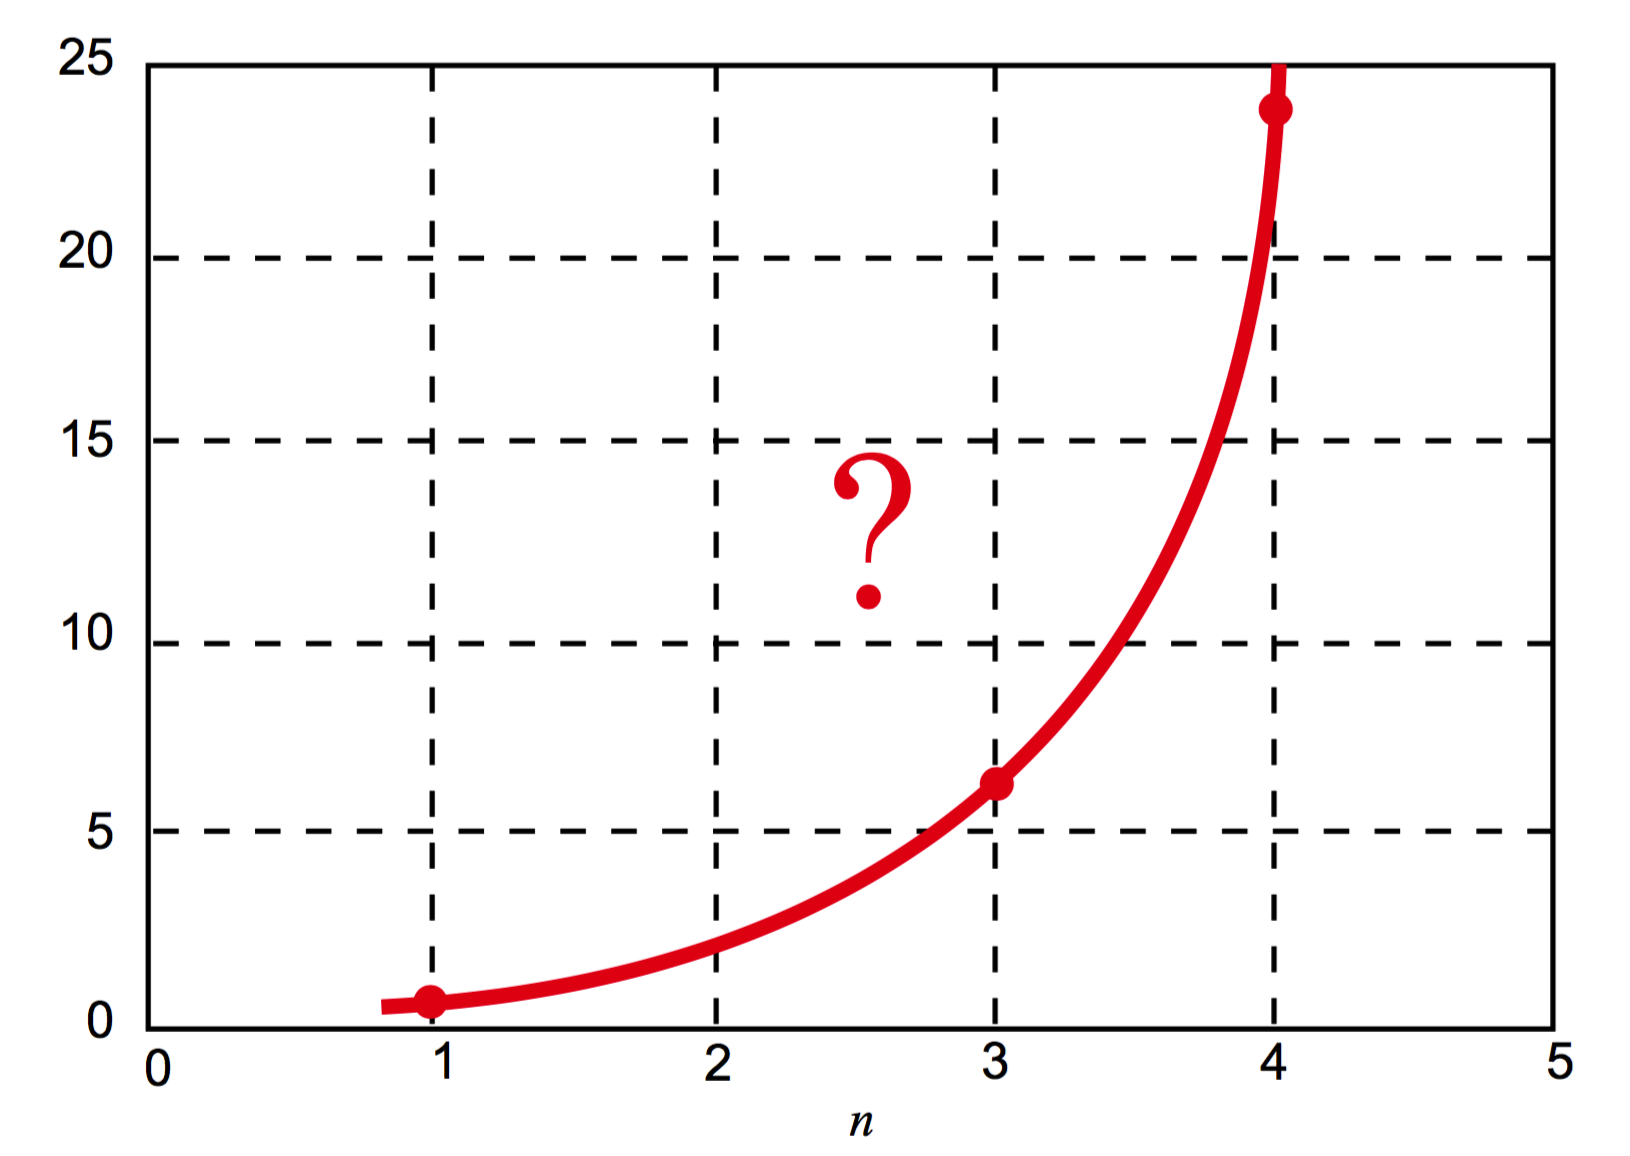
\includegraphics[width=0.6\textwidth]{gamma/factorial-curve.png}
\caption{\label{factorial-curve}通过$(n,n!)$的曲线}
\end{figure}


但是$n!$这个数列的增长速度过快,如果没有计算工具的协助,要做这个序列的插值计算也
绝非易事。幸运的是对数已经被纳皮尔(John Napier, 1550-1617) 发明出来,在数值计算
上显示了神通,被科学家们广泛接纳。斯特林和棣莫弗在他们的研究中大量地使用对数做
计算,所以很自然地斯特林转而考虑对对数序列 $\log_{10} n!$ 做插值计算。 

通过插值方法并结合对数运算的技巧,斯特林计算出 $\log_{10} (10\frac{1}{2})!=
7.0755259056$, 由此得到 $(10\frac{1}{2})! = 11899423.08$。斯特林接下来的处
理非常有意思,由于原始的阶乘数列满足递归式 $T(z) = z \cdot T(z-1)$,斯特林基于
插值的原则进行推理,认为被插值的中间项 $(\frac{1}{2})!, (1\frac{1}{2})!,
(2\frac{1}{2})!  \cdots, (9\frac{1}{2})!, (10\frac{1}{2})!$ 也应该满足这个递归
式, 于是有 
$$ \left(10\frac{1}{2}\right)! = 10\frac{1}{2} \cdot
9\frac{1}{2} \cdot  \cdots \cdot  1\frac{1}{2} \cdot \left(\frac{1}{2}\right)! $$ 
上式中代入$(10\frac{1}{2})!$的值,然后计算得到 
$$\left(\frac{1}{2}\right)! = 0.8862269251 .$$
这个结果初看起来平淡无奇,然而斯特林天才地指出,上式实际上应该是
\begin{equation}
\label{half-factorial}
\left(\frac{1}{2}\right)! = \frac{\sqrt\pi}{2} .
\end{equation}
居然出现了$\pi$, 这真是一个令人惊诧的结果!

我们不太确定斯特林是如何推断出 \eqref{half-factorial} 式的,因为在斯特林的论述
中他只是把 $(\frac{1}{2})!$ 的计算结果和 $\frac{\sqrt\pi}{2}$ 做了数值比较,并
没有进行严谨的数学推导,所以看起来好像是数值对比后猜测的结果。即便如此,这也展
示了斯特林强大的数学直觉。

考虑到我们熟悉的斯特林公式是斯特林和棣莫弗共同创造的,斯特林要利用他的插值
过程更加严谨地推导这个结果其实也很容易,虽然没有证据表明斯特林做过这种推导。
基于斯特林对 $\log_{10} n!$ 的插值处理方法,如果我们只是使用一次多项式(即直线
)做插值处理,那么中间项的插值就是两端的算术平均
$$ \log_{10} \left(n+\frac{1}{2}\right)! = \frac{\log_{10} n! + \log_{10} (n+1)!}{2} .$$
所以
$$ \left(n+\frac{1}{2}\right)! = \sqrt{n! (n+1)!} = n! \sqrt{n+1} ,$$
把递归式 $T(z) = z \cdot T(z-1)$ 应用于 $(n+\frac{1}{2})!$ 可以得到
$$ \left(n+\frac{1}{2}\right)! 
= (n+\frac{1}{2}) \cdot (n-\frac{1}{2}) \cdots \frac{3}{2} \cdot \left(\frac{1}{2}\right)! .$$
利用斯特林公式推导可以得到
\begin{align*}
\left(\frac{1}{2}\right)! & = \frac {n! \sqrt{n+1}} {(n+\frac{1}{2}) 
\cdot (n-\frac{1}{2}) \cdots \frac{3}{2}} \\
& = \frac {\sqrt{n+1} \cdot 2^{2n} \cdot n! \cdot n!} {(2n+1)!}  \\
& \displaystyle \approx \displaystyle \frac {\sqrt{n+1} \cdot 2^{2n}  
\cdot \sqrt{2\pi n} (\frac{n}{e})^n \cdot \sqrt{2\pi n} (\frac{n}{e})^n} 
{\sqrt{2\pi(2n+1)} (\frac{2n+1}{e})^{2n+1}} \\
& = \displaystyle \frac{\sqrt\pi}{2} \cdot \frac{e}{(1+\frac{1}{2n})^{2n}}  
\cdot \frac{\sqrt{2n+2}\cdot 2n}{\sqrt{2n+1}\cdot (2n+1)} \\
& \rightarrow \frac{\sqrt\pi}{2} \hspace{0.5cm} (n \rightarrow \infty) .
\end{align*}

\begin{figure}[htbp]
\centering
\includegraphics[width=0.4\textwidth]{gamma/stirling_grave.jpg}
\caption{斯特林的墓碑}
\end{figure}

斯特林的插值研究成果发表于1730年出版的《Methodus Differentialis》中,原书由拉丁
文写成,数学工作者把它翻译成了英文,并对斯特林的研究成果提供评论,使得我们有机会
追寻斯特林研究的原始足迹。 基于强大的斯特林公式,斯特林可以对$n!$ 进行便捷的近
似计算,进一步基于多项式插值的思路,斯特林也已经可以近似计算$n$为分数时的阶乘。
然而斯特林的思路遗憾地停留在数值近似计算上,没有把 $n!$ 到分数的延拓更细致地追
究下去。

% http://math.stackexchange.com/questions/109305/how-much-of-stirling-is-in-stirlings-formula
% knuth Why Pi

\section{三封信---伽玛函数的诞生}

在十七、十八世纪通讯不发达的年代,信在科学家的沟通交流中承载了极其重要的作用。
大量著名的科学研究成果是在科学家的私人笔记、朋友通信之中被首次记录的, 甚至许多
重要的研究成果都尘封在笔记、信件之中未被正式发表。因此大师的笔记、信件都成了
科学史研究的重要资料。 伽玛函数这个重要的数学函数, 在数学史上的首次现身就是在
数学家的信件中。

当斯特林着迷于他的阶乘插值研究的时候, 无独有偶,同一时代的另一位数学家哥德巴赫,几
乎在同一时间也在思考阶乘推广到分数的问题。哥德巴赫的名字在中国可以说是家喻户晓。由于
中国数学家在数论领域的杰出成就,和素数相关的哥德巴赫猜想作为数学皇冠上的明珠就
一直吸引着无数中国人的目光。 哥德巴赫一生对数列的插值问题都保持浓厚的兴趣,他很
早就开始考虑阶乘的插值问题。不同于斯特林的思路,哥德巴赫并不满足于近似数值计算
,而是希望能找到一个简洁的通项公式,既可以准确地描述整数的阶乘$n!$, 又能够推广到分数情形
。做了一些努力尝试之后哥德巴赫发现自己无法解决这个问题。幸运的是他交友广泛,和
当时许多著名的数学家都有联系,包括莱布尼茨以及数学史中出了最多位数学家的贝努利
家族。分数阶乘的问题困恼哥德巴赫多年,他不停地思考,也时常请教他的朋友。
1722 年他找尼古拉斯·贝努利讨论,不过没有取得实质性进展; 1729年他又把问题呈现
给了尼古拉斯的弟弟丹尼尔·贝努利,丹尼尔于当年10月给哥德巴赫的一封信中
给出了漂亮的解答。

\begin{figure}[htbp]
\centering
\includegraphics[width=0.3\textwidth]{gamma/goldbach2.jpg}
\quad\quad
\includegraphics[width=0.3\textwidth]{gamma/Daniel_Bernoulli_by_Grooth.jpg}
\caption{哥德巴赫和丹尼尔·贝努利}
\end{figure}


丹尼尔解决分数阶乘的思路非常漂亮:{\bf 突破有限,取道无穷!} 不拘泥于有限,而是
直接跳跃到无穷乘积的形式来考虑阶乘的插值。丹尼尔发现,如果 $m,n$都是正整数,当 $m
\rightarrow \infty$时,有
$$ \frac{1\cdot 2\cdot 3 \cdots m}{(1+n)(2+n)\cdots (m-1+n)}(m+\frac{n}{2})^{n-1} 
\rightarrow n! .$$
利用这个无穷乘积的方式可以把$n!$的定义自然地延拓到实数集。例如,取 $n=2.5$, $m$
足够大,基于上式就可以近似计算出 $2.5!$;而当$m$趋向无穷的时候,上式的极限就是
$2.5!$的精确值。丹尼尔是如何灵光乍现想到用无穷乘积的思路去解决问题的,我们无从
知晓。他能够从有限插值的围墙中跳出,足以显示他优秀的数学才能。无穷在整个数学发
展史中发挥着巨大的作用,笔者不敢妄加评论二十世纪之后的数学,然而如果说“无穷是
数学发展的发动机”,在二十世纪之前,这句评论应该不会过分。历次数学危机是因为无
穷而产生,几次数学的重大进展和飞跃也是由于数学家更加深刻地认识了无穷。 

丹尼尔的这封信成功地解决了整数阶乘到分数的推广问题,它犹如濛濛细雨,唤醒了伽玛
函数的种子,只是种子还很虚弱,在土中默默地等待着一位数学大师的灌溉。

年轻的欧拉当时正和丹尼尔·贝努利一块在圣彼得堡,他也因此得知了分数阶乘的问题。
欧拉和贝努利家族有着深厚的渊源,他是约翰·贝努利 (Johann Bernoulli, 1667-1748)
的学生, 这位约翰也就是尼古拉斯和丹尼尔的父亲。我们应该感谢约翰·贝努利,正是他
发现并培养了欧拉的数学才能。 在尼古拉斯和丹尼尔的推荐之下,年轻的欧拉于1727年在圣
彼得堡科学院获得了一个职位。受到丹尼尔·贝努利的思路的启发,欧拉也采用无穷乘积
的方式给出了另外一个$n!$ 的公式
\begin{equation}
\label{euler-series}
\Bigl[\Bigl(\frac{2}{1}\Bigr)^n\frac{1}{n+1}\Bigr]
\Bigl[\Bigl(\frac{3}{2}\Bigr)^n\frac{2}{n+2}\Bigr]
\Bigl[\Bigl(\frac{4}{3}\Bigr)^n\frac{3}{n+3}\Bigr] \cdots = n! .
\end{equation}
用极限形式,这个式子可以写为
\begin{equation}
\label{euler-series2}
\lim_{m \rightarrow \infty} \frac{1\cdot 2\cdot 3 \cdots m}{(1+n)(2+n)\cdots (m+n)}(m+1)^{n} = n!
\end{equation}
欧拉实际上在他的论文中描述了发现上述式子的思路,我们不在此赘述。上式成立其实
很容易证明。左边可以整理为
\begin{align*}
& \frac{1\cdot 2\cdot 3 \cdots m}{(1+n)(2+n)\cdots (m+n)}(m+1)^{n}  \\
= & \frac{1\cdot 2\cdot 3 \cdots n \cdot (n+1)(n+2) \cdots m}{(1+n)(2+n)\cdots m (m+1)(m+2)\cdots (m+n)}
     (m+1)^{n} \\
= & 1\cdot 2\cdot 3 \cdots n \cdot \frac{(n+1)(n+2) \cdots m}{(1+n)(2+n)\cdots m }
     \cdot \frac{(m+1)^{n}}{(m+1)(m+2)\cdots (m+n)} \\
= & n! \cdot \frac{(m+1)^{n}}{(m+1)(m+2)\cdots (m+n)} \\
= & n! \cdot \prod_{k=1}^{n} \frac{m+1}{m+k}  \\
\rightarrow & n! \qquad (m\rightarrow \infty)
\end{align*}
所以 \eqref{euler-series}、\eqref{euler-series2}式都成立。

由于\eqref{euler-series} 式对于$n$为分数的情形也适用,所以欧拉实际上也把$n!$
的计算推广到了分数的情形。欧拉给的无穷乘积相比丹尼尔的无穷乘积有什么更出色的地
方吗?实际上后人的验证指出,就收敛到$n!$的速度而言,丹尼尔的无穷乘积比欧拉的要
快得多,然而欧拉的无穷乘积公式却是能够下金蛋的鸡。 欧拉极其擅长数学的观察与归纳
,他开始尝试从一些简单的例子做分数阶乘的计算,看看是否有规律可循。当
$n=\frac{1}{2}$ 的时候,代入 \eqref{euler-series} 式,可以得到
\begin{align*}
\Bigl(\frac{1}{2}\Bigr)! 
= & \sqrt{\frac{2}{1}} \cdot \frac{2}{3} \cdot \sqrt{\frac{3}{2}} \cdot \frac{4}{5} 
    \cdot \sqrt{\frac{4}{3}} \cdot \frac{6}{7} \cdot \sqrt{\frac{5}{4}} \cdot \frac{8}{9} 
    \cdot \cdots  \\
= & \sqrt{\frac{4}{2}} \cdot \frac{2}{3} \cdot \sqrt{\frac{6}{4}} \cdot \frac{4}{5}
    \cdot \sqrt{\frac{8}{6}} \cdot \frac{6}{7} \cdot \sqrt{\frac{10}{8}} \cdot \frac{8}{9} 
    \cdot \cdots  \\
= & \sqrt{\frac{4}{3} \cdot \frac{2}{3}} \cdot \sqrt{\frac{6}{5} \cdot \frac{4}{5}}
    \cdot \sqrt{\frac{8}{7} \cdot \frac{6}{7}} \cdot \sqrt{\frac{10}{9} \cdot \frac{8}{9}} 
    \cdot \cdots  \\
= & \sqrt{\frac{2}{3} \cdot \frac{4}{3} \cdot \frac{4}{5} \cdot \frac{6}{5}
    \cdot \frac{6}{7} \cdot \frac{8}{7} \cdot \frac{8}{9} \cdot \frac{10}{9} \cdot \cdots } . 
\end{align*}
对照一下根号内的式子和沃利斯公式\eqref{wallis-formula},几乎是一模一样!只是最
前面差了一个因子2。 欧拉自然非常熟悉沃利斯的工作,基于沃利斯公式,欧拉迅速得到了
一个令他惊讶的结果
$$ \Bigl(\frac{1}{2}\Bigr)! = \frac{\sqrt{\pi}}{2} .$$

\begin{figure}[htbp]
\centering
\includegraphics[width=0.8\textwidth]{gamma/euler-swiss-banknote.jpg}
\caption{瑞士法郎上的欧拉}
\end{figure}

真是殊途同归!对于阶乘在分数$\frac{1}{2}$上的推广,欧拉得到了和当年斯特灵相同的结
果。 欧拉继续尝试计算更多分数的阶乘。 欧拉给的无穷乘积也满足阶乘的递归式$T(z)
= z T(z-1)$, 结合递归式欧拉计算了其它几个分数,包括 $\frac{5}{2}, \frac{1}{4},
\frac{3}{4}, \frac{1}{8}, \frac{3}{8} $ 的阶乘。在丹尼尔的鼓励之下,欧拉把自己
的公式以及一些分数阶乘的计算结果写信告知了哥德巴赫,这封信开启了欧拉和哥德
巴赫之间一生的通信交流。两人在接下来的 35 年里连续通信达到196封,这些信函成为了
数学家研究欧拉的重要资料。也正是哥德巴赫激发了欧拉对数论的兴趣,著名的哥德巴赫
猜想的首次现身就是在哥德巴赫写给欧拉的一封信中。

欧拉的这封信把分数阶乘的问题,又扎实地向前推进了一步。 犹如一场春雨,随风潜入夜
,润物细无声,伽玛函数的种子在土里发芽了,它积蓄着力量,等待着最后的灌溉和破土
而出。

欧拉是具有超凡数学直觉的一流数学家,他注意到 $ (\frac{1}{2})!$ 中居然有 $\pi$,
这引起他的深思。
对于擅长数学分析的数学家而言,有 $\pi$ 的地方必然有和圆相关的积分。由于沃利斯的
时代微积分理论还没有被系统地发明出来,沃利斯使用插值的方式做推导计算,但是沃利斯
公式的推导过程本质上就是在处理积分。因此欧拉猜测 $n!$ 应该可以表达为某种积分形
式。如果说沃利斯当年发现他的公式只是无心插柳,那后继者欧拉对于阶乘向分数推广的
研究将开垦出一片绿洲。 

受沃利斯工作的启发,欧拉开始考虑如下一般形式的积分
$$ J(e,n) = \int_0^1 x^e(1-x)^ndx ,$$
此处 $n$ 为正整数,$e$ 为正实数。利用分部积分法,很容易证明
$$ J(e,n) = \frac{n}{e+1}J(e+1,n-1) .$$
重复使用上述迭代公式,最终可以得到
$$ J(e,n) = \frac{1\cdot2\cdots n}{(e+1)(e+2)\cdots(e+n+1)} .$$
于是欧拉得到如下一个重要的式子
\begin{equation}
n! = (e+1)(e+2)\cdots(e+n+1)\int_0^1 x^e(1-x)^ndx .
\end{equation}
在这个公式里欧拉实际上已经成功地把$n!$ 表示成了积分的形式。然而
$(e+1)(e+2)\cdots(e+n+1)$ 这个表达式限制了 $n$ 只能为整数,无法推广到分数的情形
。能否简化这个积分表达式,让$e$ 从积分式子中消失呢?要让一个量从一个数学等式中
消失,数学家惯用的手法之一就是让这个量取一个极端的值,譬如无穷。在通往无穷的路
途中,宇宙的奥秘往往被数学家窥视。欧拉开始通过数学变换技巧让$e$ 趋向于无穷取值。
取
$e=\frac{f}{g}$, 稍微整理一下可以得到
$$ \frac{n!}{(f+g)(f+2g)\cdots(f+ng)} = \frac{f+(n+1)g}{g^{n+1}} \int_0^1 x^\frac{f}{g}(1-x)^n dx , $$
然后令 $f \rightarrow 1, g \rightarrow 0$,显然上式左边趋于$n!$, 右边会发生什么
情况呢?为了简化计算,令 $x=t^h, h=\frac{g}{f+g}$, 整理之后上式可以变换为
\begin{align}
\frac{n!}{(f+g)(f+2g)\cdots(f+ng)}
& = \frac{f+(n+1)g}{g^{n+1}} \int_0^1 h(1-t^h)^n dt  \notag \\
& = \frac{f+(n+1)g}{(f+g)^{n+1}} \int_0^1 \Bigl(\frac{1-t^h}{h}\Bigr)^n dt .
\label{factorial-integral}
\end{align}
当$f \rightarrow 1, g \rightarrow 0$ 时显然有$h \rightarrow 0$,利用罗必塔法则
,我们可以得到微积分中一个熟知的式子
$$ \lim_{h \rightarrow 0} \frac{1-t^h}{h} = -\log t .$$
由此,对 \eqref{factorial-integral} 式两边取极限,奇迹出现了:
\begin{equation}
\label{factorial-gamma-1}
n! = \int_0^1 (-\log t)^ndt .
\end{equation}
原来积分式中的$e$消失了,欧拉成功地把$n!$表达为了一个非常简洁的积分形式!!!
对上式再做一个变换 $t=e^{-\lambda}$,就得到我们常见的伽玛函数形式
\begin{equation}
\label{factorial-gamma-2}
 n! = \int_0^{\infty} \lambda^ne^{-\lambda}d\lambda .
\end{equation}
把\eqref{factorial-gamma-1}和\eqref{factorial-gamma-2} 式从正整数$n$ 延拓到任意实
数$x$,我们就得到伽玛函数的一般形式
$$ \Gamma(x+1) = \int_0^1 (-\log t)^{x}dt =  \int_0^{\infty} t^{x}e^{-t}dt .$$
1730年 欧拉把他推广得到的$n!$的积分形式再次写信告知了哥德巴赫,欧拉的这封信犹如
春雷惊起千年蛰,伽玛函数破土而出,年仅23岁的欧拉完美地解决了困扰哥德巴赫多年的
分数阶乘的问题。而伽玛函数这颗嫩芽生命力旺盛,在接下来的几百年中,将接受众多的
数学大师们的灌溉培育,开始茁壮成长。 

\begin{figure}[htbp]
\centering
\includegraphics[width=0.7\textwidth]{lda/gamma-func.png}
\caption{$\Gamma(x)$ 在正半轴的图像}
\end{figure}

回味欣赏一下欧拉推导伽玛函数的过程,我们会觉得整个过程清晰、流畅、自然,这就是
欧拉做数学研究的风格。 欧拉和高斯都是历史上具有超凡直觉的一流数学家,但是两位数
学大师做数学研究的风格却迥然不同。高斯在数学上严谨细致,呈现研究结果小心谨慎。
他的格言是 “当一幢建筑物完成时,应该把脚手架拆除干净”。所以发表研究结果的时候
常把思考的痕迹抹去,只留下那些漂亮、令人惊叹、却难以追根溯源的结果,这招致了一
些数学家对高斯的批评。
而欧拉的风格不同,他经常通过经验直觉做非常大胆的猜测,然后小心细致地求证,欧拉
的文章中留下了许多做数学猜想的痕迹,中间的证明的过程有时不够严谨,但是最
终的结论却极少出错。欧拉总是把最基本的东西解释得尽量清楚,讲明引导他得出结论的
思路。他的数学技巧超凡脱俗,时常把看似不相关的数学式子糅合在一起变换出惊人而富
有创造性的结论, 读者要理解他的思路与结论却并不困难。
拉普拉斯曾说过:“读读欧拉 ,他是我们所有人的老师。”
而高斯的评价是:“学习欧拉的著作,乃是认识数学的最好工具。”
数学家波利亚在他的名著《数学与猜想》中列举了许多欧拉做数学研究的例子,对欧拉做
数学归纳和猜想的方式推崇备至。

\begin{figure}[htbp]
\centering
\includegraphics[width=0.4\textwidth]{gamma/euler_cup.jpg}
\caption{欧拉的数学发现}
\end{figure}

欧拉被称为分析学的化身,在分析学中,无出其右者。欧拉的老师约翰·贝努利在给欧拉
的信中这样评价欧拉的工作:“ 我介绍高等分析的时候,它还是个孩子,而你正在将它带
大成人。” 希尔伯特说“分析学是无穷的交响曲”,欧拉显然是无穷分析中最出色的作曲
家。欧拉二百多年前写的教科书《无穷分析引论》至今还在不断地印刷,最近也刚刚出版
了中文翻译版本。布尔巴基学派的灵魂人物韦伊( Andr\'{e} Weil, 1906-1998) 1979 年
在 Rochester大学的一次讲演中说:“今天的学生从欧拉的《无穷分析引论》中所能得到
的益处,是现代任何一本数学教科书都比不上的。”

许多人把数学比作音乐,把欧拉称作数学界的贝多芬。因为贝多芬在两耳失聪之后继续
谱写了大量著名的交响曲,而欧拉在60岁左右双目失明之后仍然以口述形式完成了几本书
和 400 多篇论文,在数学上变得更加多产。 数学界从1911年开始出版《欧拉全集》,耗
费了一个世纪的时间,已经出版了70余卷, 25000多页, 而这项庞大的出版任务还仍处于
未完成状态。

\section{$ \Gamma(n) = (n-1)!$ 还是  $ \Gamma(n) = n! $ ? }

伽玛函数找到了,我们来看看第二个问题,为何伽玛函数被定义为满足
$\Gamma(n)=(n-1)!$? 如果我们对参数稍微做一点移位修正,把伽玛函数定义中的 $t^{x-1}$
替换为 $t^x$ 
$$ \Gamma(x) = \int_0^{\infty} t^{x}e^{-t}dt , $$
使得伽玛函数满足$\Gamma(n)=n!$,这样不是更加自然吗? 这个问题也是理科背景的学生
学习高等数学的时候的FAQ(Frequently Asked Question) ,然而答案却一直有些争议。  

伽玛函数被发现以后,在早期的数学文献中的形态并不统一。实际上,欧拉最早引入的伽玛
函数定义还真是如上所示,满足 $\Gamma(n)=n!$。而高斯在研究伽玛函数的时候, 是用
符号$\Pi$来定义: 
$$ \Pi(x)=\int_{0}^\infty t^x e^{-t}\,dt ,$$ 
不过这个定义并没有流传开来。伽玛函数在数学界的形态的最终统一要归功于勒让德。

\begin{figure}[htbp]
\centering
\includegraphics[width=0.3\textwidth]{gamma/Legendre.jpg}
\caption{勒让德肖像水彩画}
\end{figure}

欧拉在伽玛函数的推导中实际上引入了两类积分形式
$$ \int_0^1 t^{x}(1-t)^{y}dt, \quad  \quad \int_0^{\infty} t^{x}e^{-t}dt .$$
现在分别称为欧拉第一类积分和欧拉第二类积分。勒让德追随欧拉的脚步,发表了多篇论
文对欧拉积分进行了深入的研究和推广。有意思的是,在勒让德的研究中,对积分中的参
数做了 $-1$的移位修改,定义为
$$ B(x, y) = \int_0^1 t^{x-1}(1-t)^{y-1}dt, \quad \quad  \Gamma(x) = \int_0^{\infty} t^{x-1}e^{-t}dt .$$
$B(x,y)$ 现在称为贝塔积分或者贝塔函数。而基于上式的伽玛函数定义导
致了 $ \Gamma(n) = (n-1)!$ , 这同时也是首次引入$\Gamma$符号给伽玛函数冠名。勒让德
给出的伽玛函数定义被法国数学家广泛采纳并在世界范围推广,最终使得这个定义在现
代数学中成为了既成事实。

什么原因驱使勒让德选择$\Gamma(n) = (n-1)!$ 的定义呢? 这成为一个谜,没有明确的
解释。 数学史研究者们对欧拉的研究表明,在$1730\sim1768$ 年之间,欧拉自己在研究一
类积分的时候,对积分参数做了$-1$的移位修改,从而明确地引入了贝塔积分,而这个修
改显然被勒让德注意到了。 什么原因使欧拉和勒让德引入$-1$ 移位修改呢? 后来的数学
家们给出了一些猜测,一个可能的原因是这两位数学大师注意到,按照现代伽玛函数的定义,那
么
\begin{equation}
\label{beta-gamma-decompose}
 B(x,y) = \frac{\Gamma(x)\Gamma(y)}{\Gamma(x+y)} ,
\end{equation}
$B(x,y)$ 具有非常漂亮的对称形式。如果选取高斯给出的 $\Pi(n)=n!$ 的定义,
则有
$$ B(x,y) = \frac{\Pi(x)\Pi(y)}{\Pi(x+y+1)} ,$$
这个形式显然不如\eqref{beta-gamma-decompose} 式具有简洁的对称美,数学家总是非常
在乎数学公式的美感的。

还有一个类似的解释是从抽象代数的角度提出的,考虑伽玛分布的概率密度函数
$$ f_\alpha(x)=\begin{cases} \dfrac{x^{\alpha-1} e^{-x}}{\Gamma(\alpha)} 
& , x>0 \\[12pt] 0 & , x<0 \end{cases} $$
形成的集合 $\{f_\alpha : \alpha > 0\}$, 那么该集合在卷积运算 $*$ 之下构成一
个抽象代数中的半环,即满足
$$ f_\alpha * f_\beta = f_{\alpha+\beta} .$$
采用$\Pi(x)$ 的定义则无法得到类似的结果。 


对于伽玛函数定义中$-1$参数移位的合理性,现代数学家还提供了一个额外的解释,当然
这个解释和欧拉、勒让德的选择并无关系。这个更具启发性的解释也是从抽象代数角度描
述的。 对伽玛函数
$$ \Gamma(x) = \int_0^{\infty} e^{-t}t^{x-1}dt $$
做一个线性变换 $h: t \rightarrow ct$,可以得到如下函数
\begin{equation}
\label{generalized-gamma}
\frac{\Gamma(x)}{c^x}  = \int_0^{\infty} e^{-ct} t^x \frac{dt}{t} . 
\end{equation}
此处, $dt/t = d \log t$ 可以被看成是乘法群 $(0, \infty)$ 上的一个不变测度,在尺
度伸缩变换下满足不变性:
$$ \frac{d(ct)}{ct} = \frac{dt}{t} .$$
而积分式中的 $e^{-ct}$ 对应于群上的一个加法特征(additive character) $f$, 满足 
$$f(t+s) =f(t) \cdot f(s) ,$$ 
$t^x$ 对应于群上的一个乘法特征(multiplicative character) $g$, 满足
$$g(t \cdot s) = g(t) \cdot g(s) .$$
由于积分表示的是求和, 所以\eqref{generalized-gamma} 式 被看成是乘法群 $(0,
\infty)$ 上加法特征和乘法特征混合乘积的累积求和。基于这个分解,只要在抽象代数的
有限域上定义了$f$ 和$g$ 这两个映射, \eqref{generalized-gamma} 式中在实数域上定
义的$\frac{\Gamma(x)}{c^x}$ 函数就可以被推广到有限域上进行定义,只是无限求和的
积分号$\int$ 需要被替换为有限求和符号$\Sigma$ 。 进一步,借用贝塔函数和伽玛函数
满足的关系式\eqref{beta-gamma-decompose}, $B(x,y)$ 也可以完全类似的在有限域中定
义, 这种推广也同样具有简洁的对称美。


\section{伽玛函数欣赏}

伽玛函数从它诞生开始就备受青睐,众多数学大师们对它追逐研究,包括高斯、勒让德、魏
尔斯特拉斯、柳维尔等等。数学家发现这个函数拥有大量奇特的性质,为解决众多重要的
数学问题搭建了桥梁。 

由于阶乘存在一个斯特林公式,所以伽玛函数作为阶乘的推广,首先也满足如下的斯特林公式
$$ \Gamma(x) \approx \sqrt{2\pi}e^{-x}x^{x-\frac{1}{2}} .$$

数是我们在数学中接触的最普通的概念,人类对数系的认识的道路上却布满了荆棘与坎
坷。从整数、分数、有理数到无理数、实数、虚数、复数,这些数的概念的理解却是累积
了千年的沉淀,背后隐藏了多少代数学家的汗水。数学家对数的思考常常拥有惊世骇俗
的思维:每一个实数都可以计算阶乘, {\bf 那复数可以计算阶乘吗?} 数学家给我们提供
了神奇的答案:我们不仅可以计算 $ (-7.5)!, (\frac{1}{2})!,\pi !$ ,我们甚至可以
计算 $(\frac{1}{2} + \frac{1}{3}i)!$。阶乘的概念居然可以延拓到复数,这真是太
不可思议! 其实理由很简单: 因为积分的概念可以被延拓到整个复平面上。实际上,十
八世纪的数学家们着手开垦复变函数论这片沃土之后,基于积分定义的伽玛函数被延拓到
整个复平面上自然就不足为奇了。


\begin{figure}[H]
\centering
\includegraphics[width=0.6\textwidth]{lda/gamma-complex.png}
\caption{复平面上的伽玛函数}
\end{figure}

除了阶乘,伽玛函数貌似离我们很遥远,日常生活中看不到它的影子。其实伽玛函数栖身
于众多我们熟悉的事物之中。譬如,我们最为常见的圆、球就和伽玛函数紧密相关。我们
知道二维球(圆)的面积为 $\pi r^2$,三维球的体积为 $\frac{4}{3} \pi r^3$,那半径
为$r$ 的$n$维球的体积是多少呢? 这个体积是如下多重积分
$$ \displaystyle V_n(r) = \idotsint\limits_{ \tiny \{(x_1, \cdots, x_n) | \sum x_i^2 < r^2 \} }  1 \quad dx_1dx_2 \cdots dx_n  .$$
这个计算需要一点想象力,实际上可以很容易地证明 \footnote{在 Wikipedia 上可以找到一个很有启发性的证明方法。}
$$ V_n(r) = \frac{\pi^{\frac{n}{2}} r^n}{\Gamma(\frac{n}{2} + 1)} .$$ 
瞧,$n$维球体积公式完全依赖于伽玛函数,我们日常熟悉的圆的面积、球的体积公
式不过是它的特例而已。 

\begin{figure}[htbp]
\centering
\includegraphics[width=0.5\textwidth]{gamma/n-dim-ball.jpg}
\caption{$n$ 维球的体积}
\end{figure}


伽玛函数还有很多妙用,它能扩展一些重要的数学概念,譬如导数。我们学习过一阶、
二阶等整数阶导数,而数学家却追问一个令人脑洞大开的问题:{\bf 我们能定义分数阶的
导数吗?} 这个问题太令人难以捉摸了,恐怕读者们完全无法想象什么叫分数阶的导数。 
然而这个问题却历史悠久,早年莱布尼茨研究微积分的时候就提出来过这个问题,只是没
有获得实质性进展。欧拉给出了伽玛函数之后,也开始研究分数阶导数的问题,并给出了
如下非常具有启发性的想法。我们观察一下函数$f(x) = x^n$ 的各阶导数
\begin{table}[H]
\centering
\caption{$x^n$ 的各阶导数}
\begin{tabular*}{0.8\textwidth}{@{\extracolsep{\fill}}cl}
\\
$f'(x)$ & $nx^{n-1}$ \\
$f''(x)$ & $n(n-1)x^{n-2}$ \\
$f^{(3)}(x)$ & $n(n-1)(n-2)x^{n-3}$ \\
$\cdots$ &  \\
$f^{(k)}(x)$ & $n(n-1)(n-2)\cdots(n-k+1)x^{n-k} = \frac{n!}{(n-k)!} x^{n-k}$. 
\end{tabular*}
\end{table}
上式最后一行,我们发现$k$阶导数是用阶乘来表达,于是可以用伽玛函数重写为
$$ f(x)^{(k)} = \frac{\Gamma{(n+1)}}{\Gamma{(n-k+1)}} x^{n-k} .$$
伽玛函数大显身手的机会来了!基于上式,取$n=1, k=\frac{1}{2}$ 我
们就可以计算 $f(x)=x$ 的 $\frac{1}{2}$阶导数为
$$ x^{(\frac{1}{2})} = \frac{\Gamma{(1+1)}}{\Gamma{(1-1/2+1)}} x^{1-1/2} 
= \frac{2\sqrt{x}}{\sqrt{\pi}} .$$
显然以上计算过程对于$n, k$ 为任意实数的情形都适用,于是我们就很自然地把$x^n$的
导数的定义从整数阶延拓到分数阶。

那一般的可导函数$f(x)$ 可以定义分数阶导数吗? 一般的函数 $f(x)$ 可以通过泰
勒级数展开表达为幂级数,所以欧拉很容易想到借用 $x^n$ 的分数阶导数来定
义出任意可导函数的分数阶导数。这种简单的方式确实能够处理不少函数,遗憾的是在某
些函数上由于不能满足收敛性要求,因而定义是失效的。虽然欧拉没能够在函数的分数阶导
数的问题上进一步深入,但是他的这个思路给后来的数学家打开了一道门,这门通向数学
分析中的一个神奇的世界:分数微积分 (Fractional Calculus) 。一般可导函数的分数阶
导数在这个世界中都是有意义的,{\bf 甚至积分运算也可以有分数阶},因为积分运算是
导数的逆运算。这听起来是不是很有趣?而伽玛函数正是开启这道奇妙之门的魔法钥匙。 


数学家擅长刨根问底,从各个角度考察他们发现和创造的数学实体。 整数阶乘被欧拉推
广到伽玛函数之后,紧接着被问的一个问题是:{\bf 伽玛函数是整数阶乘唯一的推广函数
吗?} 答案却是否定的,丹尼尔·贝努利最早的无穷乘积推广就已经说明了存在多种推广延拓的
方式。譬如$\Gamma(x) \cos (2x\pi)$ 这个函数显然也满足把阶乘延拓到实数集。 
那伽玛函数凭什么鹤立鸡群、集万千数学家的宠爱于一身呢?从伽玛函数的图像我们可
以看到它是一个凸函数。凸函数是数学家们宠爱的对象,一个函数是凸函数往往意味着
它有众多良好的性质。那伽玛函数是唯一的满足凸性的阶乘函数吗?答案还是否定的。但
是数学家发现不仅 $\Gamma(x)$ 是一个凸函数, $\log\Gamma(x)$ 也是一个凸函数,这
可是难得一见的优良品质。实际上可以证明如下定理:
\begin{theorem}[Bohr-Mollerup] 如果 $f:(0,\infty)\rightarrow (0,\infty)$,且满足
\begin{enumerate}
\item $f(1) = 1$
\item $f(x+1) = xf(x)$
\item $\log f(x)$ 是凸函数
\end{enumerate}
那么 $f(x) = \Gamma(x)$。
\end{theorem}
一言以蔽之:伽玛函数拥有优良血统,它是唯一的在取对数后还满足凸性的阶乘推广函数。

\begin{figure}[H]
\centering
\includegraphics[width=0.6\textwidth]{lda/digamma-func.png}
\caption{$\log \Gamma(x)$ 是一个凸函数}
\end{figure}

伽玛函数像是一位神奇的魔术师,时常从黑色帽子中拉出活蹦乱跳的兔子,令人惊诧不已。
伽玛函数有不少等价的表示形式和神奇的结果。高斯给出的伽玛函数的形式是
$$ \Gamma(x) = \lim_{n\rightarrow\infty} \frac{n^x n!}{x(x+1)(x+2)\cdots(x+n)} .$$
欧拉证明了如下一个漂亮的反射公式
$$ \Gamma(x) \Gamma(1-x) = \frac{\pi}{\sin (\pi x)} .$$
看!伽玛函数和我们最为熟悉的三角函数发生了紧密的关联。
魏尔斯特拉斯把高斯的伽玛函数形式简单地做一下变换,就得到表达为无穷乘积的如下结果
$$ {\Gamma(x)} = \frac{1}{xe^{\gamma x}} \prod_{k=1}^\infty
\frac{e^{\frac{x}{k}}} {1+\frac{x}{k}} .$$
此处 $\gamma \approx 0.5772156649\cdots$ 为欧拉常数。这个结果在复平面上也成立。
由伽玛函数的这个分解形式的启发,魏尔斯特拉斯发现复平面上任意整函数$f(z)$ 都可
以分解为无穷乘积形式。之前在介绍沃利斯公式的时候,提到了欧拉发现的
$\sin x$ 的无穷乘积展开式 \eqref{euler-sinx} ,我们也说过这个展开式的证明并不算
简单。实际上,基于魏尔斯特拉斯这个伽玛函数的无穷乘积形式和欧拉的反射公式,
整理简化一下 $\Gamma(1+x)\Gamma(1-x)$, 就可以得到对 \eqref{euler-sinx} 式的
一个简洁的证明。

数论号称数学上的皇冠。伽玛函数看起来和数论八竿子打不着,却在这顶皇冠之中熠熠生
辉。 伽玛函数和欧拉常数 $\gamma$ 有密切关系,可以发现
$$ \gamma = -\frac{d\Gamma(x)}{dx}|_{x=1} =
\lim_{n\rightarrow \infty}(1+\frac{1}{2} + \frac{1}{3}+\cdots+\frac{1}{n} - \log n) . $$
欧拉常数$\gamma$ 是一个神奇的常数,它到底是一个有理数还是一个
无理数?数学家至今都耿耿于怀。进一步还可以发现伽玛函数和黎曼Zeta函数
$$ \zeta(s) = 1+\frac{1}{2^s} + \frac{1}{3^s} + \cdots $$
有着密切联系。黎曼发现了如下式子
$$ \zeta(x) \Gamma(x) = \int_0^\infty \frac{u^{x-1}}{e^u - 1} du ,$$
$$ \zeta(x) = \zeta(1-x) \Gamma(1-x) 2^s \pi^{s-1} \sin\left(\frac{\pi x}{2}\right)  .$$
这可了不得! $\zeta$ 函数在解析数论中有着举足轻重的地位,它涉及了数学中极其著
名的素数分布定理和黎曼猜想,而以上两个式子在分析黎曼猜想过程中有重要作用。数学
家蒙哥马利有一句名言:“假如你是一个魔鬼,引诱数学家用自己的灵魂来换取一个定理
的证明。多数数学家会想要换取的会是什么定理呢,我想会是黎曼猜想。” 而希尔伯特曾
说过,如果他在沉睡1000年后醒来, 他将问的第一个问题便是:黎曼猜想得到证明了吗?

前面提到了 $\log\Gamma(x)$ 是一个凸函数。对这个函数求导得到的函数
$$ \Psi(x) = \frac{d\log\Gamma(x)}{dx}  $$
被称为 Digamma 函数。可以证明
$$\Psi(x) = -\gamma + (x-1) - \frac{(x-1)(x-2)}{2\cdot 2!} 
+ \frac{(x-1)(x-2)(x-3)}{3\cdot 3!} \cdots $$
这也是一个很重要的函数,具有如下漂亮的性质
$$ \Psi(x+1) = \Psi(x) + \frac{1}{x} .$$
基于这个递归性质,把上式在正整数上作递归展开就得到调和级数 $1+\frac{1}{2} +
\frac{1}{3} + \frac{1}{4} + \cdots $,所以$\Psi(x)$ 在调和级数研究中扮演重要角
色。 进一步,函数$\Psi(x)$和欧拉常数$\gamma$ 以及 $\zeta$ 函数都有密切关系。令
$$ \Psi_n(x) = \frac{d^{n+1}\log\Gamma(x)}{dx^{n+1}} ,$$
可以证明
$$\Psi_1(x) = \frac{d^{2}\log\Gamma(x)}{dx^{2}}
= \frac{1}{x^2} + \frac{1}{(x+1)^2} + \frac{1}{(x+2)^2} + \cdots .$$
对于几个具体的数值,有如下漂亮的结果
$$\Psi(1) = -\gamma, \quad \quad \Psi(2) = 1-\gamma ,$$
$$\Psi_1(1) = \zeta(2) = 1 + \frac{1}{2^2} + \frac{1}{3^2} + \frac{1}{4^2} +  \cdots 
= \frac{\pi^2}{6} .$$


\section{随机数学中的伽玛函数}

伽玛函数在概率统计中频繁现身,众多的统计分布,包括常见的统计学三大分布($t$ 分布
,$\chi^2$ 分布,$F$ 分布)、贝塔分布、狄利克雷分布的密度公式中都有伽玛函数的
身影。当然发生最直接联系的概率分布是直接由伽玛函数变换得到的伽玛分布。对伽玛函
数的定义做一个变形,可以得到如下式子
\begin{equation}
\label{gamma-distribution}
\int_0^{\infty} \frac{x^{\alpha-1}e^{-x}}{\Gamma(\alpha)}dx = 1 .
\end{equation}
取上式积分号中的函数作为概率密度,就得到一个形式最简单的伽玛分布密度函数
$$Gamma(x|\alpha) = \frac{x^{\alpha-1}e^{-x}}{\Gamma(\alpha)} .$$
如果在\eqref{gamma-distribution} 式中做变换 $x=\beta t$, 就得到伽玛分布密度
函数更一般的形式
$$Gamma(t|\alpha, \beta) = \frac{\beta^\alpha t^{\alpha-1}e^{-\beta t}}{\Gamma(\alpha)} .$$

\begin{figure}[htbp]
\centering
\includegraphics[width=0.6\textwidth]{lda/gamma-distribution.png}
\caption{\label{gamma-distr-graph}$ Gamma(\alpha,\beta)$分布图像}
\end{figure}

伽玛分布在概率统计领域也是一个万人迷,众多概率分布都和它有密切关系。 我们熟悉
的指数分布$Exp(\lambda)$和$\nu$个自由度的卡方分布 $\chi^2_{(\nu)}$ 其实都是
伽玛分布的特例,密度函数分别对应于 $Gamma(1, \lambda)$ 和
$Gamma(\frac{\nu}{2}, \frac{1}{2})$ 。 观察图 \ref{gamma-distr-graph} 可以发现
,伽玛分布在不同的参数配置下可以呈现众多的形状,因此具有强大的拟合数据的能力。
伽玛分布同时是一个很强大的先验分布,在贝叶斯统计分析中被广泛地用作其它分布的先
验。如果把统计分布中的共轭关系类比为人类生活中的情侣关系的话,那指数分布、泊松
分布、正态分布、对数正态分布都可以看作是伽玛分布的情人。

接下来的内容中我们主要关注$\beta = 1$的简单形式的伽玛分布。伽玛分布首先和泊松分
布发生密切的联系。容易发现伽玛分布和泊松分布在数学形式上具有高度的一致性。参数
为$\lambda$的泊松分布,概率分布写为
$$Poisson(X=k|\lambda) = \frac{\lambda^k e^{-\lambda}}{k!} , $$
在伽玛分布的密度函数中取 $\alpha = k+1$ 得到
$$ Gamma(\lambda|\alpha=k+1) 
= \frac{\lambda^ke^{-\lambda}}{\Gamma(k+1)}= \frac{\lambda^k e^{-\lambda}}{k!} . $$
这二者一模一样!这两个分布的数学形式具有高度的一致性。只是泊松分布是离散的,伽玛分布
是连续的。这种数学上的一致性难道是偶然的吗? 事实上,从泊松分布出发,利用一
个简单的概率物理模型可以对伽玛分布的密度函数给出清晰的物理解释。

泊松分布可以用于描述一段时间内事件发生次数的统计性质,譬如接到的电话的次数。假
设我们关心的不是一段有限的时间,而是 $(0, \infty)$ 整个时间轴上接到电话的统计性
质,应该如何来描述呢?我们可以假设接到的电话满足如下性质
\begin{enumerate}
\item 概率在时间轴是独立均匀分布的,即每个等长的时间区间上是否接到电话是独立的
,并且概率分布一样;每一个长度为h的充分小的时间片上接到一个电话的概率正比于时间
片的长度;
\item 每一个充分小时间片上最多只能接到一个电话;
\item 平均而言,假设每个长度为1的单位时间片上接到电话个数是1。
\end{enumerate}
如果我们考察 $[0, \lambda]$ 这个时间区间,那么平均而言,这个长度为 $\lambda$ 的
时间片上应该接到 $\lambda$ 个电话,把这个时间区间分成 $n$ 个独立的小片,那么每
个时间片上接到一个电话的概率恰好是 $p = \lambda/n$。当$n$ 足够大的时候,每个时
间片上只能接到一个电话或者没有接到电话,恰好对应于成功概率为$p$ 的一个贝努利
实验。于是$n$ 个时间片对应于$n$ 个独立的贝努利实验,所以 $[0, \lambda]$这个时间
区间上接到的电话总数$X$ 应该符合二项分布
$$p(X=k) = \binom{n}{k} p^k(1-p)^{n-k} .$$
由于 $np= \lambda$, 当 $n$ 趋向于无穷的时候,电话个数$X$将满足参数为
$\lambda$ 的泊松分布
$$p(X=k) = \frac{\lambda^k e^{-\lambda}}{k!} .$$

熟悉随机过程理论的读者马上会发现以上模型实际上是参数为1 的泊松过程。 我们关心的
问题是:什么时候会接到第${k+1}$ 个电话?或者说{\bf 接到第$k+1$ 个电话的时间点
$Y_{k+1}$ 会是什么概率分布?} 形式化的描述就是如何计算如下概率
$$ P(\lambda < Y_{k+1} \le \lambda +  d\lambda) = ? .$$
上式的含义是第$k+1$ 个电话落在长度为 $d\lambda$ 的区间 $(\lambda, \lambda +
d\lambda] $ 内,这个概率事件可以分解为两个独立事件
\begin{enumerate}
\item 区间 $(\lambda, \lambda +  d\lambda] $ 内接到一个电话,这个概率是 $d \lambda .$ (由于这个时间片足够小,按照题目要求,也只能接到一个电话.)
\item 区间 $[0, \lambda]$ 内接到了前$k$ 个电话,这个概率是 
$$ p(X=k) = \frac{\lambda^k e^{-\lambda}}{k!} .$$
\end{enumerate}
于是所求的概率是以上两个事件概率相乘,即
$$ P(\lambda < Y_{k+1} \le \lambda +  d\lambda) = p(X=k) \cdot d \lambda .$$
由于第$k+1$ 个电话必然出现在时间轴上某处,所以把时间轴所有无穷小区间上的概率累
加起来,正好对应于必然事件的概率1,所以有
$$ \int_0^\infty  p(X=k) \cdot d \lambda  = 1 .$$
把$P(X=k)$ 代入上式即可得到 
$$ \int_0^\infty \frac{\lambda^k e^{-\lambda}}{k!}  d \lambda  = 1 ,$$
$$ k! = \int_0^\infty \lambda^k e^{-\lambda} d \lambda .$$
上述两式正好就对应于伽玛分布和伽玛函数对阶乘的推广。所以,{\bf  接到第$k+1$ 个
电话的时间点 $Y_{k+1}$ 恰好符合伽玛分布}。 综上, 我们其实是从泊松分布出发,完
全基于概率物理模型,推导出了伽马分布和伽玛函数,而推导的过程给伽玛分布的密度函
数提供了很好的物理解释。

如果我们把$e^\lambda$的泰勒展开式和伽玛函数对照写成如下形式:
\begin{align}
e^\lambda & =  \sum_{k=0}^{\infty} {\lambda^k \over k!} , \\
k! & =  \int_0^{\infty} {\lambda^k \over e^\lambda}\ d\lambda ,
\end{align}
我们发现这两个式子形式上具有对偶关系。由于 $\sum$ 和$\int$ 都表示求和, 几乎可
以认为从第一个式子只是把 $e^\lambda$ 和 $k!$ 交换一下就得到了第二个式子。 这两
个式子之间有更多的内在联系吗?事实上如下一个奇妙的等式成立:
\begin{equation}
\label{gamma-e-taylor}
\frac{1}{k!} \int_0^\lambda \frac{\lambda^k}{e^\lambda} d\lambda 
+ \frac{1}{e^\lambda} \sum_{n=0}^k \frac{\lambda^n}{n!} = 1 .
\end{equation}

用上面描述的泊松过程的物理模型,可以很容易的证明这个等式。我们把数轴分成
$(0, \lambda]$ 和 $(\lambda, \infty)$ 这两个区间,考察第$k+1$ 个电话接到的时间
$Y_{k+1}$ 分别落在这两个区间的概率,当然有
$$ P(Y_{k+1} \le \lambda) + P(Y_{k+1} > \lambda)  = 1 .$$
按照上述的物理模型,显然第$k+1$ 个电话的时间落入$(0, \lambda]$ 的概率为
$$ P(Y_{k+1} \le \lambda) = \int_0^\lambda \frac{\lambda^k e^{-\lambda}}{k!}  d \lambda .$$
如果第$k+1$ 个电话的时间点落入 $(\lambda, \infty)$,这个事件等价地可以理解为 $(0,
\lambda]$ 上的电话个数不能超过 $k$ 个,由于$(0, \lambda]$ 这个有限时间区间上的
电话次数符合参数为$\lambda$ 的泊松分布, 所以这个概率为
$$  P(Y_{k+1} > \lambda) = Poisson(X \le k|\lambda) = \sum_{n=0}^k \frac{\lambda^n e^{-\lambda} }{n!} .$$
所以我们得到
\begin{equation}
\label{poisson-gamma-dual}
\int_0^\lambda \frac{\lambda^k e^{-\lambda}}{k!}d\lambda 
+ \sum_{n=0}^k \frac{\lambda^n e^{-\lambda}}{n!} = 1 .
\end{equation}
这个式子俗称{\bf 泊松-伽玛对偶},将它简单整理一下就是 \eqref{gamma-e-taylor} 式。

由于泊松分布可以看做是二项分布的极限分布,我们也可以从二项分布的角度对伽玛
分布进行解释。由于 
$$ e^{-\lambda} = \lim_{n\rightarrow \infty} (1- \frac{\lambda}{n}) ^n ,$$
所以伽玛分布的概率密度可以重写为
\begin{align*}
\frac{\lambda^k e^{-\lambda}}{k!} 
& = \lim_{n\rightarrow \infty} \frac{\lambda^k (1-\frac{\lambda}{n}) ^n}{k!}  \\
& = \lim_{n\rightarrow \infty} \frac{ n! n^k (\frac{\lambda}{n})^k (1-\frac{\lambda}{n}) ^n}{k! \cdot n!} \\
& = \lim_{n\rightarrow \infty} \frac{(n+k)!}{k!\cdot n!} (\frac{\lambda}{n})^k (1-\frac{\lambda}{n}) ^n  \\
& = \lim_{n\rightarrow \infty} \binom{n+k}{k} (\frac{\lambda}{n})^k (1-\frac{\lambda}{n}) ^n  .
\end{align*}
显然上式具有明确的二项分布的物理含义。进一步,二项分布和贝塔分布之间也存在完全
类似\eqref{poisson-gamma-dual} 的一个等式:
\begin{equation}
\label{binomial-beta-dual}
\frac{n!}{k!(n-k-1)!} \int_0^p t^k(1-t)^{n-k-1} dt + \sum_{v=0}^k \binom{n}{v} p^v(1-p)^{n-v} = 1 .
\end{equation}
事实上我们知道$n\rightarrow\infty$时上式中二项分布的极限是泊松分布,而贝塔分布的
极限是伽玛分布,那么就很容易理解 \eqref{poisson-gamma-dual} 其实可以看做是
\eqref{binomial-beta-dual} 的极限形式。 

\section{结语}


作家海明威有一句名言:“冰山运动之雄伟壮观,是因为它只有八分之一在水面上。”阶
乘这个基于整数的数学概念,俨然是一座冰山宫殿!整数的一角漂浮于水面之上,朴实无
华,迷惑了众人的眼睛。满怀好奇心的数学探险家们却眼光犀利深邃, 洞察了那水下的奥
秘。 在深入细致地分析探索中, 探险家们来到了深藏于冰山深处的一个深邃而庞大的洞穴
入口 --- 那是神奇的伽玛函数的宫殿之门。 数学探险家们争先恐后进入洞穴一窥究竟,
却不识庐山真面目,几代探险家们的努力下终于发现这是一座雄伟壮观的冰山宫殿,宫殿的
基石由实数域、复数域、甚至是有限域搭建而成, 屋顶由整数铺设,宫殿深藏于水中,微
微露出一角。 殿中有众多迷人的现代数学宫室, 琳琅满目地陈列着伽玛函数的神奇技艺
,令人赏心悦目、流连忘返。 

\begin{figure}[t]
\centering
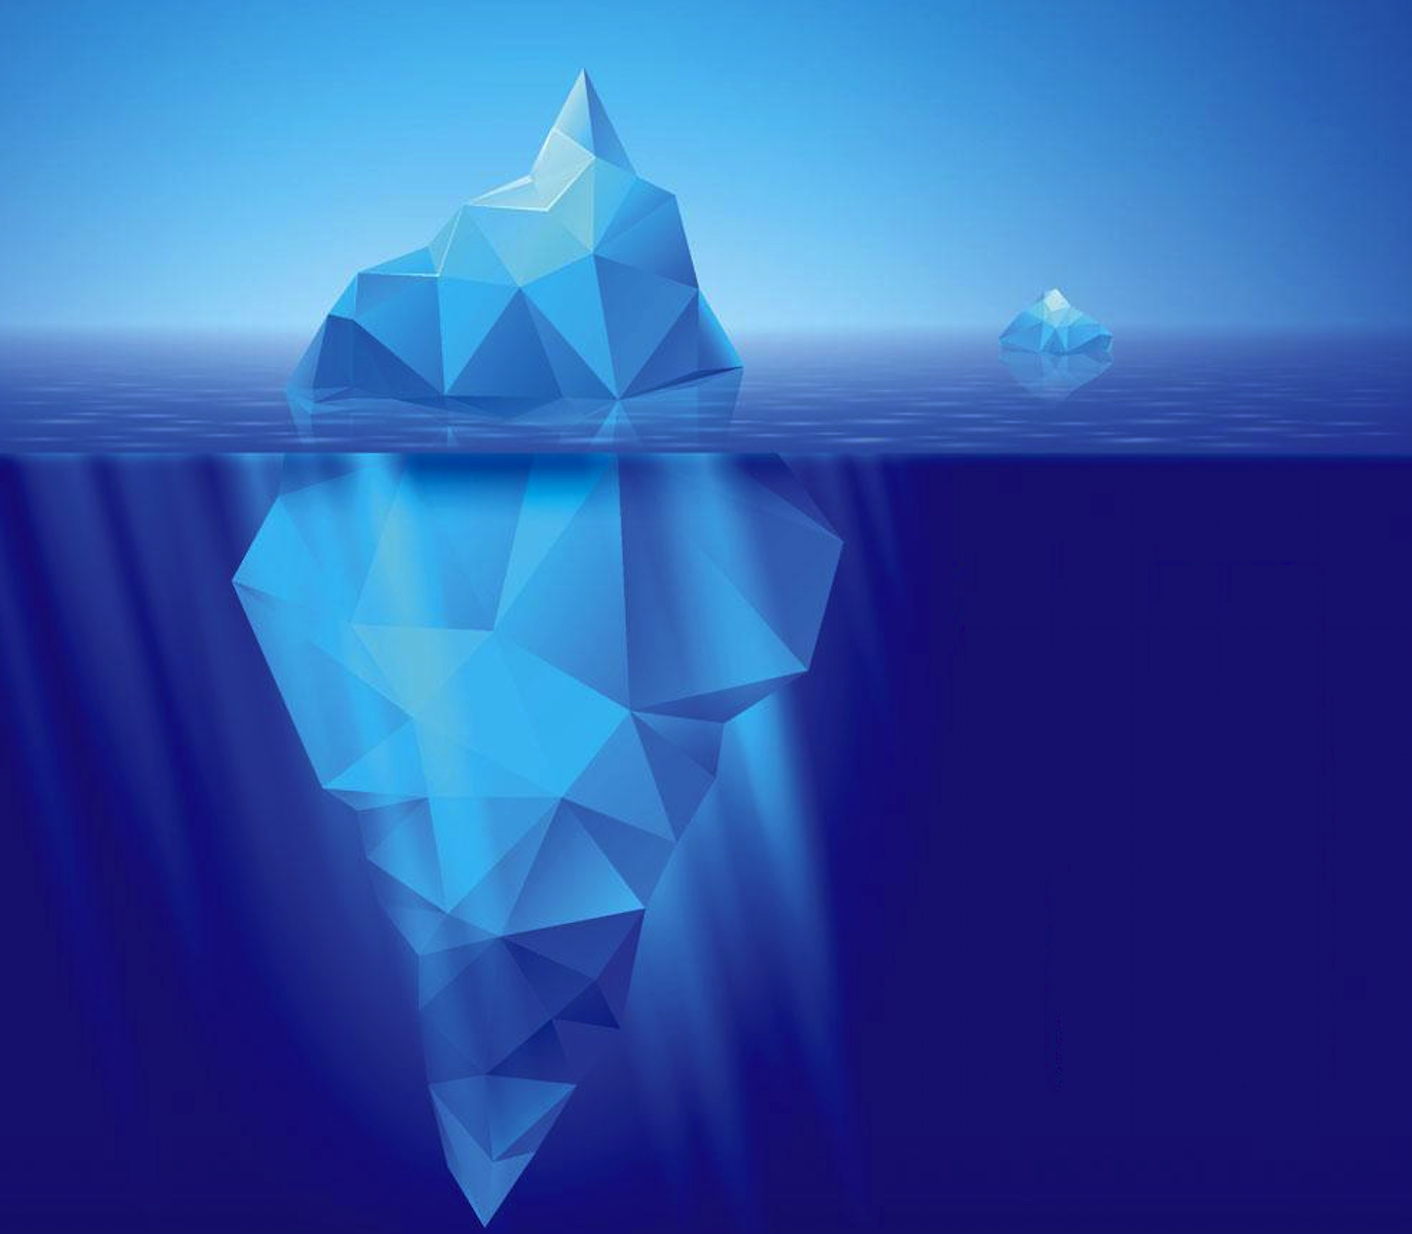
\includegraphics[height=0.5\textwidth, width=0.8\textwidth]{gamma/iceberg.png}
\caption{伽玛函数冰山}
\end{figure}

许多人认为数学的概念是静态的:数学概念产生于历史上某一个时刻,某一位数学大家之
手,之后就几乎一成不变了。对于大多数非数学专业的人而言,这种感觉很自然,毕竟普
通读者所接触的几何、代数、微积分这些数学知识早就已经体系成熟,存在了几百甚至上
千年。 然而数学的发展其实是先有探索的阶段,然后才会沉淀为逻辑与体系,只是我们的
数学课本历来偏重后者而忽视前者。如果我们对数学知识的探索过程有所了解的话,会发
现这些探索也犹如冰山掩藏在水面之下的部分,甚至比露出的尖角还更具魅力。 

台湾的数学教授蔡聪明先生在数学的科普传播方面写过大量的文章,他在《数学的发现趣
谈》一书中对于数学的创造、发现与发展有一段精彩的论述:“如果你不知道一个定理(
或公式)是怎样发现的,那么你对它并没有真正的了解,因为真正的了解必须从逻辑因果
掌握到创造的心理因果。一个定理的诞生,基本上跟一粒种子在适当的土壤、风雨、阳光
、气候 ... 之下,发芽成一颗树,再开花结果,并没有两样。”本文尝试尽可能的呈现伽
玛函数这颗数学之树的生长历程,可以说伽玛函数的种子最早是沃利斯播下的,欧拉给予
了最好的施肥、灌溉使得种子发芽,而后来众多数学家的努力使得这颗嫩芽茁壮成长,
最终几乎成长为一颗参天大树。

伽玛函数这颗大树在现代数学中如此繁茂,笔者知识浅薄仅能描绘它很有限的一部分。这
个函数在数学上魅力独特,不仅能够被一个理科本科生很好的理解,它本身又足够的深刻
,具有很多漂亮的数学性质,历史上曾吸引了众多一流的数学家对它进行探索研究。美国数
学家 Philip J.Davis 在1959年的《美国数学月刊》上发表了一篇很有名的介绍伽玛函数
的文章,文中对伽玛函数一些特性发现的历史进行了详细的描述,这篇文章获得了
Chauvenet Prize (美国数学会颁发的数学科普奖)。 他在文章的末尾做了一句总结, 我把
它理解为那是对神奇的伽玛函数由衷的赞美和认同:

\begin{quotation}
\noindent
\emph{Each generation has found something of interest to say about the gamma
function.  Perhaps the next generation will also.}
\kaishu{(每一代人都发现了一些伽玛函数的有趣性质,也许下一代人也会有所发现。)}
\end{quotation}


\section{推荐阅读}

如果希望了解更多阶乘研究以及伽玛函数相关的历史,推荐阅读如下文献:
\begin{itemize}
\item 蔡聰明, 瓦里斯尋$\pi$ 的發現理路,科学月刊, 27(4) 1996
\item 蔡聰明, 瓦里斯公式及其相關的結果,科学月刊, 27(5), 1996 
\item 蔡聰明, 談 Stirling 公式, 数学传播 , 17(2), 1993
\item Philip J. Davis, Leonhard Euler's Integral: A Historical Profile of the Gamma Function, The American Mathematical Monthly, vol. 66, pp. 849-869, 1959 
\item Jacques Dutka, The Early History of the Factorial Function, Archive for History of Exact Sciences, 43 (3), pp. 225-249, 1991
\item Detlef Gronnau, Why is the gamma function so as it is?, Teaching Mathematics and Computer Science, 2003
\item Emil Artin, The Gamma function(English Traslation),  Holt, Rinehart and Winston, Inc., 1964
\item George E. Andrews et al., Special Functions, Cambridge University Press, 2001
\item Ian Tweddle, James Stirling's Methodus Differentialis: An Annotated Translation of Stirling's Text, Springer, 2003
\end{itemize}
% bibliogrphaphy


% 考虑用到最后的总结中
% 法国伟大的数学家庞加莱(Poincare, 1854-1912)说过:我们用逻辑来证明,但是用直觉
% 来发现。逻辑…是不孕的,除非它跟直觉受精。


% !Mode:: "TeX:UTF-8"
% Author: Rickjin (ZhihuiJin@gmail.com)
%
\chapter{认识Beta/Dirichlet分布}
\section{撒旦的游戏---认识Beta 分布}

统计学就是猜测上帝的游戏,当然我们不总是有机会猜测上帝,运气不好的时候就得揣度魔鬼的心思。
有一天你被魔鬼撒旦抓走了,撒旦说:“你们人类很聪明,而我是很仁慈的,
和你玩一个游戏,赢了就可以走,否则把灵魂出卖给我。
游戏的规则很简单,我有一个魔盒,上面有一个按钮,你每按一下按钮,
就均匀的输出一个[0,1]之间的随机数,我现在按10下,
我手上有10个数,你猜第7大的数是什么,偏离不超过0.01就算对。” 你应该怎么猜呢?

从数学的角度抽象一下,上面这个游戏描述如下
\begin{algorithm}[H]
\floatname{algorithm}{Game}
\caption{猜测第$k$ 大的数}
\begin{algorithmic}[1]
\STATE $X_1,X_2,\cdots,X_n {\stackrel{\mathrm{iid}}{\sim}} Uniform(0,1)$,
\STATE 把这$n$ 个随机变量排序后得到顺序统计量 $X_{(1)},X_{(2)},\cdots, X_{(n)}$,
\STATE 问 $X_{(k)}$ 的分布是什么
\end{algorithmic}
\end{algorithm}
对于不喜欢数学的同学而言,估计每个概率分布都是一个恶魔,那在概率统计学中,
均匀分布应该算得上是潘多拉魔盒,几乎所有重要的概率分布都可以从均匀分布$Uniform(0,1)$中生成出来。
\begin{figure}[htbp]
\centering
\includegraphics[width=0.6\textwidth]{lda/pandora.jpg}
\caption{潘多拉魔盒}
\end{figure}

对于上面的游戏而言 $n=10,k=7$, 如果我们能求出 $X_{(7)}$ 的分布的概率密度,那么用概率密度的极值点
去做猜测就是最好的策略。对于一般的情形,$X_{(k)}$ 的分布是什么呢?那我们尝试计算一下$X_{(k)}$ 落在
一个区间 $[x, x+\Delta x]$ 的概率,也就是求如下概率值
$$ P( x \le X_{(k)} \le x+\Delta x) = ? $$

把 [0,1] 区间分成三段 $[0,x), [x,x+\Delta x], (x+\Delta x,1]$,
我们先考虑简单的情形,假设$n$ 个数中只有一个落在了区间 $[x, x+\Delta x]$内,
则因为这个区间内的数$X_{(k)}$是第$k$大的,则$[0,x)$中应该有 $k-1$ 个数,$(x,1]$这个区间中应该有
$n-k$ 个数。不失一般性,我们先考虑如下一个符合上述要求的事件$E$
\begin{align*}
 E = \{ & X_1 \in [x, x+\Delta x],  \\
 & X_i \in [0,x)\quad (i=2,\cdots,k), \\
 & X_j \in (x+\Delta x,1] \quad (j=k+1,\cdots,n)\}
\end{align*}
\begin{figure}[htbp]
\centering
\includegraphics[width=0.8\textwidth]{lda/beta-game-1.png}
\caption{事件 $E$}
\end{figure}

则有
\begin{align*}
 P(E) & = \prod_{i=1}^nP(X_i) \\
 & = x^{k-1}(1-x-\Delta x)^{n-k}\Delta x \\
 & = x^{k-1}(1-x)^{n-k}\Delta x + o(\Delta x)
\end{align*}
$o(\Delta x)$表示$\Delta x $的高阶无穷小。
显然,由于不同的排列组合,即$n$个数中有一个落在 $[x, x+\Delta x]$区间的有$n$种取法,余下
$n-1$个数中有$k-1$个落在$[0,x)$的有$\binom{n-1}{k-1}$种组合,所以和事件$E$等价的事件一共有
$n\binom{n-1}{k-1}$个。

继续考虑稍微复杂一点情形,假设$n$ 个数中有两个数落在了区间 $[x, x+\Delta x]$,
\begin{align*}
E' = \{ & X_1,X_2\in [x, x+\Delta x], \\
& X_i \in [0,x) \quad (i=3,\cdots,k), \\
& X_j \in (x+\Delta x,1] \quad (j=k+1,\cdots,n)\}
\end{align*}
\begin{figure}[htbp]
\centering
\includegraphics[width=0.8\textwidth]{lda/beta-game-2.png}
\caption{事件 $E'$}
\end{figure}

则有
$$ P(E') = x^{k-2}(1-x-\Delta x)^{n-k}(\Delta x)^2 = o(\Delta x)$$

从以上分析我们很容易看出,只要落在$[x, x+\Delta x]$内的数字超过一个,
则对应的事件的概率就是 $o(\Delta x)$。于是
\begin{align*}
& P( x \le X_{(k)} \le x+\Delta x) \\
& = n\binom{n-1}{k-1}P(E) + o(\Delta x) \\
& = n\binom{n-1}{k-1}x^{k-1}(1-x)^{n-k}\Delta x +  o(\Delta x)
\end{align*}
所以,可以得到$X_{(k)}$的概率密度函数为
\begin{align*}
f(x) & = \lim_{\Delta x \rightarrow 0} \frac{P( x \le X_{(k)} \le x+\Delta x)}{\Delta x} \\
& = n\binom{n-1}{k-1}x^{k-1}(1-x)^{n-k} \\
& = \frac{n!}{(k-1)!(n-k)!}x^{k-1}(1-x)^{n-k} \quad x \in [0,1]
\end{align*}
利用Gamma 函数,我们可以把 $f(x)$ 表达为
$$ f(x) = \frac{\Gamma(n+1)}{\Gamma(k)\Gamma(n-k+1)}x^{k-1}(1-x)^{n-k} $$
还记得神奇的 Gamma 函数可以把很多数学概念从整数集合延拓到实数集合吧。我们在上式中取
$\alpha=k, \beta=n-k+1$, 于是我们得到
\begin{equation}
f(x) = \frac{\Gamma(\alpha+\beta)}{\Gamma(\alpha)\Gamma(\beta)}x^{\alpha-1}(1-x)^{\beta-1}
\end{equation}
这个就是一般意义上的 Beta 分布!可以证明,在$\alpha,\beta$取非负实数的时候,这个概率密度函数也都是良定义的。

好,我们回到魔鬼的游戏,这$n=10,k=7$这个具体的实例中,我们按照如下密度分布的峰值去猜测才是最有把握的。
$$ f(x) = \frac{10!}{(6)!(3)!}x^{6}(1-x)^{3} \quad x \in [0,1] $$

然而即便如此,我们能做到一次猜中的概率也不高,很不幸,你第一次没有猜中,
魔鬼微笑着说:“我再仁慈一点,再给你一个机会,你按5下这个机器,
你就得到了5个[0,1]之间的随机数,然后我可以告诉你这5个数中的每一个,和我的第7大的数相比,
谁大谁小,然后你继续猜我手头的第7大的数是多少。”这时候我们应该怎么猜测呢?

\section{Beta-Binomial 共轭}
魔鬼的第二个题目,数学上形式化一下,就是
\begin{algorithm}[htb]
\floatname{algorithm}{Game}
\caption{继续猜测第$k$ 大的数}
\begin{algorithmic}[1]
\STATE $X_1,X_2,\cdots,X_n {\stackrel{\mathrm{iid}}{\sim}}Uniform(0,1)$,排序后对应的顺序统计量 $X_{(1)},X_{(2)},\cdots, X_{(n)}$,  我们要猜测 $p=X_{(k)}$;
\STATE $Y_1,Y_2,\cdots,Y_m {\stackrel{\mathrm{iid}}{\sim}}Uniform(0,1)$, $Y_i$中有$m_1$个比$p$小,$m_2$个比$p$大;
\STATE 问 $P(p|Y_1,Y_2,\cdots,Y_m)$ 的分布是什么。
\end{algorithmic}
\end{algorithm}

由于$p=X_{(k)}$在 $X_1,X_2,\cdots,X_n $中是第$k$大的,利用$Y_i$的信息,我们容易推理得到 $p=X_{(k)}$ 在
$X_1,X_2,\cdots,X_n,Y_1,Y_2,\cdots,Y_m {\stackrel{\mathrm{iid}}{\sim}} Uniform(0,1)$ 这$(m+n)$个独立随机变量中是第 $k+m_1$大的,
于是按照上一个小节的推理,此时$p=X_{(k)}$ 的概率密度函数是 $Beta(p|k+m_1,n-k+1+m_2)$。
按照贝叶斯推理的逻辑,我们把以上过程整理如下:
\begin{enumerate}
\item $p=X_{(k)}$是我们要猜测的参数,我们推导出 $p$ 的分布为 $f(p) = Beta(p|k,n-k+1)$,称为 $p$ 的先验分布;
\item 数据$Y_i$中有$m_1$个比$p$小,$m_2$个比$p$大,$Y_i$相当于是做了$m$次贝努利实验,所以$m_1$ 服从二项分布 $B(m,p)$;
\item 在给定了来自数据提供的$(m_1,m_2)$的知识后,$p$ 的后验分布变为 $f(p|m_1,m_2)=Beta(p|k+m_1,n-k+1+m_2)$
\end{enumerate}
\begin{figure}[htbp]
\centering
\includegraphics[width=0.2\textwidth]{lda/coin-toss.jpg}
\caption{贝努利实验}
\end{figure}
我们知道贝叶斯参数估计的基本过程是
\begin{center}
 \bf{先验分布 + 数据的知识  = 后验分布}
\end{center}
以上贝叶斯分析过程的简单直观的表述就是
$$ Beta(p|k,n-k+1) + BinomCount(m_1,m_2) = Beta(p|k+m_1,n-k+1+m_2) $$
其中 $(m_1,m_2)$ 对应的是二项分布$B(m_1+m_2,p)$的计数。
更一般的,对于非负实数$\alpha,\beta$,我们有如下关系
\begin{equation}
 Beta(p|\alpha,\beta) + BinomCount(m_1,m_2) = Beta(p|\alpha+m_1,\beta+m_2)
\end{equation}
这个式子实际上描述的就是 {\bf Beta-Binomial 共轭},此处共轭的意思就是,
数据符合二项分布的时候,参数的先验分布和后验分布都能保持Beta 分布的形式,
这种形式不变的好处是,我们能够在先验分布中赋予参数很明确的物理意义,
这个物理意义可以延续到后验分布中进行解释,
同时从先验变换到后验过程中从数据中补充的知识也容易有物理解释。

而我们从以上过程可以看到,
Beta 分布中的参数$\alpha,\beta$都可以理解为物理计数,这两个参数经常被称为伪计数(pseudo-count)。
基于以上逻辑,我们也可以把$Beta(p|\alpha,\beta)$写成下式来理解
\begin{equation}
\label{uniform-beta}
Beta(p|1,1) + BinomCount(\alpha-1,\beta-1) = Beta(p|\alpha,\beta)
\end{equation}
其中 $Beta(p|1,1)$ 恰好就是均匀分布$Uniform(0,1)$。

对于\eqref{uniform-beta}式,我们其实也可以纯粹从贝叶斯的角度来进行推导和理解。
假设有一个不均匀的硬币抛出正面的概率为$p$,抛$m$次后出现正面和反面的次数分别是$m_1,m_2$,
那么按传统的频率学派观点,$p$的估计值应该为 $\hat{p}=\frac{m_1}{m}$。而从贝叶斯学派的观点来看,
开始对硬币不均匀性一无所知,所以应该假设$p\sim Uniform(0,1)$, 于是有了二项分布的计数$(m_1,m_2)$
之后,按照贝叶斯公式如下计算$p$ 的后验分布
\begin{align*}
P(p|m_1,m_2)  & = \frac{P(p)\cdot P(m_1,m_2|p)}{P(m_1,m_2)} \\
& = \frac{1\cdot P(m_1,m_2|p)}{\int_0^1 P(m_1,m_2|t)dt} \\
& = \frac{\binom{m}{m_1}p^{m_1}(1-p)^{m_2}}{\int_0^1 \binom{m}{m_1}t^{m_1}(1-t)^{m_2}dt} \\
& = \frac{p^{m_1}(1-p)^{m_2}}{\int_0^1 t^{m_1}(1-t)^{m_2}dt}
\end{align*}
计算得到的后验分布正好是 $Beta(p|m_1+1,m_2+1)$。

\begin{figure}[htbp]
\centering
\includegraphics[width=0.8\textwidth]{lda/beta-distribution.png}
\caption{百变星君Beta分布}
\end{figure}
Beta 分布的概率密度我们把它画成图,会发现它是个百变星君,它可以是凹的、凸的、单调上升的、单调下降的;
可以是曲线也可以是直线,而均匀分布也是特殊的Beta分布,读者请参看一个网站上的
\href{http://www.aiaccess.net/English/Glossaries/GlosMod/e_gm_beta_distri.htm}{Beta 分布 Demo},
通过调节参数$\alpha,\beta$ 可以观察 Beta 分布的各种形态。。由于Beta 分布能够拟合如此之多的形状,
因此它在统计数据拟合和贝叶斯分析中被广泛使用。

在上一个小节中,我们从二项分布推导Gamma 分布的时候,使用了如下的等式
\begin{equation}
\label{binomial-beta2}
P(C \le k) = \frac{n!}{k!(n-k-1)!} \int_p^1 t^k(1-t)^{n-k-1} dt,  \quad  C\sim B(n,p)
\end{equation}
现在大家可以看到,左边是二项分布的概率累积,右边实际上是$Beta(t|k+1,n-k)$ 分布的概率积分。
这个式子在上一小节中并没有给出证明,下面我们利用和魔鬼的游戏类似的概率物理过程进行证明。

我们可以如下构造二项分布,取随机变量 $X_1, X_2, \cdots, X_n {\stackrel{\mathrm{iid}}{\sim}}Uniform(0,1)$,
一个成功的贝努利实验就是 $X_i<p$,否则表示失败,于是成功的概率为$p$。
$C$用于计数成功的次数,于是$C\sim B(n,p)$。
\begin{figure}[H]
\centering
\includegraphics[width=0.8\textwidth]{lda/beta-binomial.png}
\caption{贝努利实验最多成功$k$次}
\end{figure}
显然我们有如下式子成立
$$ P(C \le k) = P(X_{(k+1)} > p)$$
此处$X_{(k+1)}$是顺序统计量,为第$k+1$大的数。
等式左边表示贝努利实验成功次数最多$k$次,右边表示第 $k+1$ 大的数必然对应于失败的贝努利实验,
从而失败次数最少是$n-k$次,所以左右两边是等价的。
由于$X_{(k+1)} \sim Beta(t|k+1, n-k)$, 于是
\begin{align*}
P(C \le k) & = P(X_{(k+1)} > p) \\
&= \int_p^1 Beta(t|k+1, n-k)dt \\
&= \frac{n!}{k!(n-k-1)!} \int_p^1 t^k(1-t)^{n-k-1} dt
\end{align*}

最后我们再回到魔鬼的游戏,如果你按出的5个随机数字中,魔鬼告诉你有2个小于它手中第7大的数,
那么你应该按照如下概率分布的峰值做猜测是最好的
$$ Beta(x|9,7) = \frac{15!}{(8)!(6)!}x^{8}(1-x)^{6} \quad x \in [0,1] $$

很幸运的,你这次猜中了,魔鬼开始甩赖了:这个游戏对你来说太简单了,
我要加大点难度,我们重新来一次,我按魔盒20下生成20个随机数,
你同时给我猜第7大和第13大的数是什么,这时候应该如何猜测呢?

\section{Dirichlet-Multinomial 共轭}
对于魔鬼变本加厉的新的游戏规则,数学形式化如下:
\begin{algorithm}[htb]
\floatname{algorithm}{Game}
\caption{猜测第$k_1$ 大和第$k_1+k_2$大的数}
\begin{algorithmic}[1]
\STATE $X_1,X_2,\cdots,X_n {\stackrel{\mathrm{iid}}{\sim}}Uniform(0,1)$,
\STATE 排序后对应的顺序统计量 $X_{(1)},X_{(2)},\cdots, X_{(n)}$,
\STATE 问 $(X_{(k_1)}, X_{(k_1+k_2)})$的联合分布是什么;
\end{algorithmic}
\end{algorithm}

完全类似于第一个游戏的推导过程,我们可以进行如下的概率计算
(为了数学公式的简洁对称,我们取$x_3$满足$x_1+x_2+x_3 = 1$,但只有$x_1,x_2$是变量)
\begin{figure}[htbp]
\centering
\includegraphics[width=0.8\textwidth]{lda/dirichlet-game.png}
\caption{$(X_{(k_1)}, X_{(k_1+k_2)})$的联合分布推导}
\end{figure}
\begin{align*}
& P\Bigl(X_{(k_1)}\in(x_1,x_1+\Delta x),X_{(k_1+k_2)}\in(x_1+x_2,x_1+x_2+\Delta x)\Bigr) \\
& = n(n-1)\binom{n-2}{k_1-1,k_2-1}x_1^{k_1-1}x_2^{k_2-1}x_3^{n-k_1-k_2}(\Delta x)^2 \\
& = \frac{n!}{(k_1-1)!(k_2-1)!(n-k_1-k_2)!}x_1^{k_1-1}x_2^{k_2-1}x_3^{n-k_1-k_2}(\Delta x)^2
\end{align*}
于是我们得到 $(X_{(k_1)}, X_{(k_1+k_2)})$的联合分布是
\begin{align*}
f(x_1,x_2,x_3) & = \frac{n!}{(k_1-1)!(k_2-1)!(n-k_1-k_2)!}x_1^{k_1-1}x_2^{k_2-1}x_3^{n-k_1-k_2} \\
& = \frac{\Gamma(n+1)}{\Gamma(k_1)\Gamma(k_2)\Gamma(n-k_1-k_2+1)}x_1^{k_1-1}x_2^{k_2-1}x_3^{n-k_1-k_2}
\end{align*}
熟悉 Dirichlet的同学一眼就可以看出,上面这个分布其实就是3维形式的 Dirichlet 分布
$Dir(x_1,x_2,x_3|k_1,k_2,n-k_1-k_2+1)$。
令 $\alpha_1=k_1,\alpha_2=k_2,\alpha_3=n-k_1-k_2+1$,于是分布密度可以写为
\begin{equation}
\displaystyle f(x_1,x_2,x_3) = \frac{\Gamma(\alpha_1 + \alpha_2 + \alpha_3)}
{\Gamma(\alpha_1)\Gamma(\alpha_2)\Gamma(\alpha_3)}x_1^{\alpha_1-1}x_2^{\alpha_2-1}x_3^{\alpha_3-1}
\end{equation}

这个就是一般形式的3维 Dirichlet 分布,即便 $\vec{\alpha}=(\alpha_1,\alpha_2, \alpha_3)$ 延拓
到非负实数集合,以上概率分布也是良定义的。

从形式上我们也能看出,Dirichlet 分布是Beta 分布在高维度上的推广,他和Beta 分布一样也是一个百变星君,
密度函数可以展现出多种形态。
\begin{figure}[htbp]
\centering
\includegraphics[width=0.8\textwidth]{lda/dirichlet-distribution.png}
\caption{不同 $\alpha$ 下的Dirichlet 分布}
\end{figure}


类似于魔鬼的游戏2,我们也可以调整一下游戏3,从魔盒中生成$m$个随机数
$Y_1,Y_2,\cdots,Y_m {\stackrel{\mathrm{iid}}{\sim}}Uniform(0,1)$
并让魔鬼告诉我们$Y_i$和$(X_{(k_1)}, X_{(k_1+k_2)})$相比谁大谁小。于是有如下游戏4
\begin{algorithm}[htb]
\floatname{algorithm}{Game}
\caption{继续猜测第$k_1$ 大和第$k_1+k_2$大的数}
\begin{algorithmic}[1]
\STATE $X_1,X_2,\cdots,X_n {\stackrel{\mathrm{iid}}{\sim}}Uniform(0,1)$,排序后对应的顺序统计量 $X_{(1)},X_{(2)},\cdots, X_{(n)}$
\STATE 令$p_1=X_{(k_1)}, p_2=X_{(k_1+k_2)},p_3 = 1-p_1-p_2$(加上$p_3$是为了数学表达简洁对称),
我们要猜测 $\vec{p}=(p_1,p_2,p_3)$;
\STATE $Y_1,Y_2,\cdots,Y_m {\stackrel{\mathrm{iid}}{\sim}}Uniform(0,1)$, $Y_i$中落到
$[0,p_1),[p_1,p_2),[p_2,1]$ 三个区间的个数分别为 $m_1,m_2,m_3$,$m=m_1+m_2+m3$;
\STATE 问后验分布 $P(\vec{p}|Y_1,Y_2,\cdots,Y_m)$ 的分布是什么。
\end{algorithmic}
\end{algorithm}

为了方便,我们记
$$ \vec{m}=(m_1,m_2,m_3),\quad \vec{k}=(k_1,k_2,n-k_1-k_2+1) $$
由游戏中的信息,我们可以推理得到 $p_1, p_2$在
$X_1,X_2,\cdots,X_n,$ $Y_1,Y_2,\cdots,Y_m$
${\stackrel{\mathrm{iid}}{\sim}} Uniform(0,1)$
这 $m+n$个数中分别成为了第 $k_1+m_1, k_2+m_2$大的数,于是后验分布 $P(\vec{p}|Y_1,Y_2,\cdots,Y_m)$
应该是 $Dir(\vec{p}|k_1+m_1,k_1+m_2,n-k_1-k_2+1+m_3)$,即
$Dir(\vec{p}|\vec{k}+\vec{m})$。
按照贝叶斯推理的逻辑,我们同样可以把以上过程整理如下:
\begin{enumerate}
\item 我们要猜测参数 $\vec{p}=(p_1,p_2,p_3)$,其先验分布为$Dir(\vec{p}|\vec{k})$;
\item 数据$Y_i$落到$[0,p_1), [p_1,p_2),[p_2,1]$三个区间的个数分别为 $m_1,m_2,m_3$,所以
$\vec{m}=(m_1,m_2,m_3)$ 服从多项分布$Mult(\vec{m}|\vec{p})$
\item 在给定了来自数据提供的知识$\vec{m}$后,$\vec{p}$ 的后验分布变为 $Dir(\vec{p}|\vec{k}+\vec{m})$
\end{enumerate}
以上贝叶斯分析过程的简单直观的表述就是
$$ Dir(\vec{p}|\vec{k}) + MultCount(\vec{m}) = Dir(\vec{p}|\vec{k}+\vec{m}) $$
令 $\vec{\alpha}=\vec{k}$,把$\vec{\alpha}$
从整数集合延拓到实数集合,更一般的可以证明有如下关系
\begin{equation}
 Dir(\vec{p}|\vec{\alpha}) + MultCount(\vec{m})
 = Dir(\vec{p}|\vec{\alpha}+\vec{m})
\end{equation}
以上式子实际上描述的就是 {\bf Dirichlet-Multinomial 共轭},而我们从以上过程可以看到,
Dirichlet 分布中的参数$\vec{\alpha}$都可以理解为物理计数。
类似于 Beta 分布,我们也可以把 $Dir(\vec{p}|\vec{\alpha})$作如下分解
$$ Dir(\vec{p}|\vec{1}) + MultCount(\vec{m}-\vec{1})
= Dir(\vec{p}|\vec{\alpha}) $$
此处$\vec{1}=(1,1,\cdots,1)$。自然,上式我们也可以类似地用纯粹贝叶斯的观点进行推导和解释。

以上的游戏我们还可以往更高的维度上继续推,譬如猜测 $X_{(1)},X_{(2)},\cdots, X_{(n)}$ 中的
4、5、...等更多个数,于是就得到更高纬度的 Dirichlet 分布和 Dirichlet-Multinomial 共轭。
一般形式的 Dirichlet 分布定义如下
\begin{equation}
\displaystyle Dir(\vec{p}|\vec{\alpha}) =
\displaystyle \frac{\Gamma(\sum_{k=1}^K\alpha_k)}
{\prod_{k=1}^K\Gamma(\alpha_k)} \prod_{k=1}^K p_k^{\alpha_k-1}
\end{equation}
对于给定的 $\vec{p}$和 $N$,多项分布定义为
\begin{equation}
\displaystyle  Mult(\vec{n} |\vec{p},N) = \binom{N}{\vec{n}}\prod_{k=1}^K p_k^{n_k}
\end{equation}
而 $Mult(\vec{n} |\vec{p},N)$ 和 $Dir(\vec{p}|\vec{\alpha})$
这两个分布是共轭关系。

Beta-Binomail 共轭和 Dirichlet-Multinomail 共轭都可以用纯粹数学的方式进行证明,我们在这两个小节中通过一个游戏
来解释这两个共轭关系,主要是想说明这个共轭关系是可以对应到很具体的概率物理过程的。

\section{Beta/Dirichlet 分布的一个性质}

如果 $p\sim Beta(t|\alpha,\beta)$, 则
\begin{align*}
E(p) & = \int_0^1 t*Beta(t|\alpha,\beta)dt \\
& =  \int_0^1 t* \frac{\Gamma(\alpha+\beta)}{\Gamma(\alpha)\Gamma(\beta)} t^{\alpha-1}(1-t)^{\beta-1}dt \\
& = \frac{\Gamma(\alpha+\beta)}{\Gamma(\alpha)\Gamma(\beta)}  \int_0^1 t^{\alpha}(1-t)^{\beta-1}dt
\end{align*}
上式右边的积分对应到概率分布 $Beta(t|\alpha+1,\beta)$,对于这个分布,我们有
$$
\int_0^1 \frac{\Gamma(\alpha+\beta+1)}{\Gamma(\alpha+1)\Gamma(\beta)} t^{\alpha}(1-t)^{\beta-1}dt = 1
$$
把上式带入$E(p)$的计算式,得到
\begin{align}
E(p) & = \frac{\Gamma(\alpha+\beta)}{\Gamma(\alpha)\Gamma(\beta)}
\cdot \frac{\Gamma(\alpha+1)\Gamma(\beta)}{\Gamma(\alpha+\beta+1)} \notag \\
& = \frac{\Gamma(\alpha+\beta)}{\Gamma(\alpha+\beta+1)}\frac{\Gamma(\alpha+1)}{\Gamma(\alpha)} \notag \\
& = \frac{\alpha}{\alpha+\beta}
\label{beta-mean}
\end{align}
这说明,对于Beta 分布的随机变量,其均值可以用$\frac{\alpha}{\alpha+\beta}$来估计。
Dirichlet 分布也有类似的结论,
如果$\vec{p} \sim Dir(\vec{t}|\vec{\alpha})$,同样可以证明
\begin{equation}
 E(\vec{p}) = \Bigl(\frac{\alpha_1}{\sum_{i=1}^K\alpha_i},\frac{\alpha_2}{\sum_{i=1}^K\alpha_i},\cdots, \frac{\alpha_K}{\sum_{i=1}^K\alpha_i} \Bigr)
 \label{dir-mean}
\end{equation}
以上两个结论很重要,因为我们在后面的 LDA 数学推导中需要使用这个结论。



% !Mode:: "TeX:UTF-8"
% Author: Rickjin (ZhihuiJin@gmail.com)
%
\chapter{MCMC 和 Gibbs Sampling}
\section{随机模拟}

随机模拟(或者统计模拟)方法有一个很酷的别名是蒙特卡罗方法(Monte Carlo Simulation)。
这个方法的发展始于20世纪40年代,和原子弹制造的曼哈顿计划密切相关,当时的几个大牛,包括
乌拉姆、冯.诺依曼、费米、费曼、Nicholas Metropolis,
在美国洛斯阿拉莫斯国家实验室研究裂变物质的中子连锁反应的时候,
开始使用统计模拟的方法,并在最早的计算机上进行编程实现。

\begin{figure}[htbp]
\centering
\includegraphics[width=0.3\textwidth]{lda/simulation.jpg}
\caption{随机模拟与计算机}
\end{figure}

现代的统计模拟方法最早由数学家乌拉姆提出,被Metropolis命名为蒙特卡罗方法,
蒙特卡罗是著名的赌场,赌博总是和统计密切关联的,所以这个命名风趣而贴切,很快被大家广泛接受。
被不过据说费米之前就已经在实验中使用了,但是没有发表。
说起蒙特卡罗方法的源头,可以追溯到18世纪,布丰当年用于计算$\pi$的著名的投针实验
就是蒙特卡罗模拟实验。
统计采样的方法其实数学家们很早就知道,但是在计算机出现以前,随机数生成的成本很高,
所以该方法也没有实用价值。随着计算机技术在二十世纪后半叶的迅猛发展,随机模拟技
术很快进入实用阶段。对那些用确定算法不可行或不可能解决的问题,蒙特卡罗方法常常为人们带来希望。

\begin{figure}[htbp]
\centering
\includegraphics[width=0.8\textwidth]{lda/monte-carlo-simulation.jpg}
\caption{蒙特卡罗方法}
\end{figure}

统计模拟中有一个重要的问题就是给定一个概率分布$p(x)$,我们如何在计算机中生成它的样本。
一般而言均匀分布 $Uniform(0,1)$的样本是相对容易生成的。 通过线性同余发生器可以生成伪随机数,
我们用确定性算法生成$[0,1]$之间的伪随机数序列后,这些序列的各种统计指标和均匀分布 $Uniform(0,1)$
的理论计算结果非常接近。这样的伪随机序列就有比较好的统计性质,可以被当成真实的随机数使用。

\begin{figure}[htbp]
\centering
\includegraphics[width=0.8\textwidth]{lda/sampling.png}
\caption{生成一个概率分布的样本}
\end{figure}

而我们常见的概率分布,无论是连续的还是离散的分布,都可以基于$Uniform(0,1)$ 的样本生成。
例如正态分布可以通过著名的 Box-Muller 变换得到
\begin{theorem}[Box-Muller 变换]
如果随机变量 $U_1, U_2$ 独立且$U_1, U_2 \sim Uniform[0,1]$,则
\begin{align*}
Z_0 & = \sqrt{-2\ln U_1} cos(2\pi U_2) \\
Z_1 & = \sqrt{-2\ln U_1} sin(2\pi U_2)
\end{align*}
则, $Z_0,Z_1$ 独立且服从标准正态分布。
\end{theorem}

其它几个著名的连续分布,包括指数分布、Gamma 分布、t 分布、F 分布、Beta 分布、Dirichlet 分布
等等,也都可以通过类似的数学变换得到;离散的分布通过均匀分布更加容易生成。
更多的统计分布如何通过均匀分布的变换生成出来,大家可以参考统计计算的书,
其中 Sheldon M. Ross 的《统计模拟》是写得非常通俗易懂的一本。

不过我们并不是总是这么幸运的,当$p(x)$的形式很复杂,或者 $p(\mathbf{x})$ 是个高维的分布的时候,
样本的生成就可能很困难了。 譬如有如下的情况
\begin{enumerate}
\item  $\displaystyle p(x) = \frac{\tilde{p}(x)}{\int \tilde{p}(x) dx}$,
而 $\tilde{p}(x)$ 我们是可以计算的,但是底下的积分式无法显式计算。
\item $p(x,y)$ 是一个二维的分布函数,这个函数本身计算很困难,
但是条件分布 $p(x|y),p(y|x)$的计算相对简单;
如果 $p(\mathbf{x})$ 是高维的,这种情形就更加明显。
\end{enumerate}

此时就需要使用一些更加复杂的随机模拟的方法来生成样本。
而本节中将要重点介绍的 MCMC(Markov Chain Monte Carlo) 和
Gibbs Sampling算法就是最常用的一种,这两个方法在现代贝叶斯分析中被广泛使用。
要了解这两个算法,我们首先要对马氏链的平稳分布的性质有基本的认识。

\section{马氏链及其平稳分布}
马氏链的数学定义很简单
$$ P(X_{t+1}=x|X_t, X_{t-1}, \cdots) =P(X_{t+1}=x|X_t) $$
也就是状态转移的概率只依赖于前一个状态。

我们先来看马氏链的一个具体的例子。社会学家经常把人按其经济状况分成3类:
下层(lower-class)、中层(middle-class)、上层(upper-class),我们用1,2,3 分别
代表这三个阶层。社会学家们发现决定一个人的收入阶层的最重要的因素就是其父母
的收入阶层。如果一个人的收入属于下层类别,那么他的孩子属于下层收入的概率是
0.65, 属于中层收入的概率是 0.28, 属于上层收入的概率是 0.07。事实上,
从父代到子代,收入阶层的变化的转移概率如下

\begin{center}
\begin{tabular}{ccccc}
\hline
& & & 子代 &  \\
& State & 1 & 2 & 3 \\
\hline
     &1 & 0.65 & 0.28 & 0.07 \\
父代 & 2 & 0.15 & 0.67 & 0.18 \\
     & 3 & 0.12 & 0.36 & 0.52 \\
\end{tabular}
\end{center}

\begin{figure}[htbp]
\centering
\includegraphics[width=0.6\textwidth]{lda/markov-transition.png}
\end{figure}

使用矩阵的表示方式,转移概率矩阵记为
$$P =
\begin{bmatrix}
0.65 & 0.28 & 0.07 \\
0.15 & 0.67 & 0.18 \\
0.12 & 0.36 & 0.52 \\
\end{bmatrix}
$$

假设当前这一代人处在下层、中层、上层的人的比例是概率分布向量 $\pi_0=[\pi_0(1), \pi_0(2), \pi_0(3)]$,
那么他们的子女的分布比例将是 $\pi_1=\pi_0P$, 他们的孙子代的分布比例将是 $\pi_2 = \pi_1P=\pi_0P^2$,
......, 第$n$代子孙的收入分布比例将是 $\pi_n = \pi_{n-1}P = \pi_0P^n$。

假设初始概率分布为$\pi_0 = [0.21,0.68,0.11] $,则我们可以计算前$n$代人的分布状况如下
\begin{center}
\begin{tabular}{clll}
第$n$代人 & 下层 & 中层 & 上层 \\
\hline
0 & 0.210 & 0.680 & 0.110 \\
1 & 0.252 & 0.554 & 0.194 \\
2 & 0.270 & 0.512 & 0.218 \\
3 & 0.278 & 0.497 & 0.225 \\
4 & 0.282 & 0.490 & 0.226 \\
5 & 0.285 & 0.489 & 0.225 \\
6 & 0.286 & 0.489 & 0.225 \\
7 & 0.286 & 0.489 & 0.225 \\
8 & 0.289 & 0.488 & 0.225 \\
9 & 0.286 & 0.489 & 0.225 \\
10 & 0.286 & 0.489 & 0.225 \\
$\cdots$  & $\cdots$  & $\cdots$  & $\cdots$  \\
\end{tabular}
\end{center}

我们发现从第7代人开始,这个分布就稳定不变了,这个是偶然的吗?
我们换一个初始概率分布$\pi_0 = [0.75,0.15,0.1]$ 试试看,继续计算前$n$代人的分布状况如下
\begin{center}
\begin{tabular}{clll}
第$n$代人 & 下层 & 中层 & 上层 \\
\hline
0 & 0.75 & 0.15 & 0.1 \\
1 & 0.522 & 0.347 & 0.132 \\
2 & 0.407 & 0.426 & 0.167 \\
3 & 0.349 & 0.459 & 0.192 \\
4 & 0.318 & 0.475 & 0.207 \\
5 & 0.303 & 0.482 & 0.215 \\
6 & 0.295 & 0.485 & 0.220 \\
7 & 0.291 & 0.487 & 0.222 \\
8 & 0.289 & 0.488 & 0.225 \\
9 & 0.286 & 0.489 & 0.225 \\
10 & 0.286 & 0.489 & 0.225 \\
$\cdots$  & $\cdots$  & $\cdots$  & $\cdots$  \\
\end{tabular}
\end{center}

我们发现,到第9代人的时候, 分布又收敛了。最为奇特的是,两次给定不同的初始概率分布,最终都收敛到
概率分布 $\pi=[0.286, 0.489, 0.225]$,也就是说收敛的行为和初始概率分布 $\pi_0$ 无关。
这说明这个收敛行为主要是由概率转移矩阵$P$决定的。我们计算一下 $P^n$
$$ P^{20} = P^{21} = \cdots = P^{100} = \cdots =
\begin{bmatrix}
0.286 & 0.489 & 0.225 \\
0.286 & 0.489 & 0.225 \\
0.286 & 0.489 & 0.225 \\
\end{bmatrix}
$$

我们发现,当 $n$ 足够大的时候,这个$P^n$矩阵的每一行都是稳定地收敛到$\pi=[0.286, 0.489, 0.225]$
这个概率分布。自然的,这个收敛现象并非是我们这个马氏链独有的,而是绝大多数马氏链的共同行为,
关于马氏链的收敛我们有如下漂亮的定理:

\begin{theorem} 如果一个非周期马氏链具有转移概率矩阵$P$,且它的任何两个状态是连通的,
那么 $\displaystyle \lim_{n\rightarrow\infty}P_{ij}^n$ 存在且与$i$无关,
记 $\displaystyle \lim_{n\rightarrow\infty}P_{ij}^n = \pi(j)$, 我们有
\begin{enumerate}
\item $ \displaystyle \lim_{n \rightarrow \infty} P^n =
\begin{bmatrix}
\pi(1) & \pi(2) & \cdots & \pi(j) & \cdots \\
\pi(1) & \pi(2) & \cdots & \pi(j) & \cdots \\
\cdots & \cdots & \cdots & \cdots & \cdots \\
\pi(1) & \pi(2) & \cdots & \pi(j) & \cdots \\
\cdots & \cdots & \cdots & \cdots & \cdots \\
\end{bmatrix} $
\item $ \displaystyle \pi(j) = \sum_{i=0}^{\infty}\pi(i)P_{ij} $
\item $\pi$ 是方程 $\pi P = \pi$ 的唯一非负解
\end{enumerate}
其中,
$$ \pi = [\pi(1), \pi(2), \cdots, \pi(j),\cdots ], \quad \sum_{i=0}^{\infty} \pi_i = 1  $$
$\pi$称为马氏链的平稳分布。
\end{theorem}


这个马氏链的收敛定理非常重要,\textbf{所有的 MCMC(Markov Chain Monte Carlo)
方法都是以这个定理作为理论基础的。}
定理的证明相对复杂,一般的随机过程课本中也不给证明,
所以我们就不用纠结它的证明了,直接用这个定理的结论就好了。我们对这个定理的内容做一些解释说明:
\begin{enumerate}
\item 该定理中马氏链的状态不要求有限,可以是有无穷多个的;
\item 定理中的“非周期“这个概念我们不打算解释了,因为我们遇到的绝大多数马氏链都是非周期的;
\item 两个状态$i,j$是连通并非指$i$ 可以直接一步转移到$j$($P_{ij} > 0$),而是指 $i$ 可以通过有限的$n$步
转移到达$j$($P_{ij}^n > 0$)。马氏链的任何两个状态是连通的含义是指存在一个$n$, 使得
矩阵$P^n$ 中的任何一个元素的数值都大于零。
\item 我们用 $X_i$ 表示在马氏链上跳转第$i$步后所处的状态,
如果 $\displaystyle \lim_{n\rightarrow\infty}P_{ij}^n = \pi(j)$ 存在,
很容易证明以上定理的第二个结论。由于
\begin{align*}
P(X_{n+1}=j) & = \sum_{i=0}^\infty P(X_n=i) P(X_{n+1}=j|X_n=i) \\
& = \sum_{i=0}^\infty P(X_n=i) P_{ij}
\end{align*}
上式两边取极限就得到 $ \displaystyle \pi(j) = \sum_{i=0}^{\infty}\pi(i)P_{ij}$
\end{enumerate}

从初始概率分布 $\pi_0$ 出发,我们在马氏链上做状态转移,记$X_i$的概率分布为$\pi_i$, 则有
\begin{align*}
X_0 & \sim \pi_0(x) \\
X_i & \sim \pi_i(x),  \quad\quad \pi_i(x) = \pi_{i-1}(x)P = \pi_0(x)P^n
\end{align*}
由马氏链收敛的定理, 概率分布$\pi_i(x)$将收敛到平稳分布 $\pi(x)$。假设到第$n$步
的时候马氏链收敛,则有
\begin{align*}
X_0 & \sim \pi_0(x) \\
X_1 & \sim \pi_1(x) \\
& \cdots \\
X_n & \sim \pi_n(x)=\pi(x) \\
X_{n+1} & \sim \pi(x) \\
X_{n+2}& \sim \pi(x) \\
& \cdots
\end{align*}
所以 $X_n,X_{n+1},X_{n+2},\cdots \sim \pi(x)$ 都是同分布的随机变量,当然他们并不独立。
如果我们从一个具体的初始状态 $x_0$ 开始,沿着马氏链按照概率转移矩阵做跳转,
那么我们得到一个转移序列 $x_0, x_1, x_2, \cdots x_n, x_{n+1}\cdots,$
由于马氏链的收敛行为, $x_n, x_{n+1},\cdots$ 都将是平稳分布 $\pi(x)$ 的样本。

\section{Markov Chain Monte Carlo}
对于给定的概率分布$p(x)$,我们希望能有便捷的方式生成它对应的样本。
由于马氏链能收敛到平稳分布, 于是一个很的漂亮想法是:如果我们能构造一个转移矩阵为$P$的马氏链,
使得该马氏链的平稳分布恰好是$p(x)$,
那么我们从任何一个初始状态$x_0$出发沿着马氏链转移, 得到一个转移序列
$x_0, x_1, x_2, \cdots x_n, x_{n+1}\cdots,$, 如果马氏链在第$n$步已经收敛了,于是我们就得到了
$\pi(x)$ 的样本$x_n, x_{n+1}\cdots$。

这个绝妙的想法在1953年被 Metropolis想到了,为了研究粒子系统的平稳性质,
Metropolis 考虑了物理学中常见的波尔兹曼分布的采样问题,首次提出了基于马氏链的蒙特卡罗方法,
即Metropolis算法,并在最早的计算机上编程实现。Metropolis 算法是首个普适的采样方法,
并启发了一系列 MCMC方法,所以人们把它视为随机模拟技术腾飞的起点。
Metropolis的这篇论文被收录在《统计学中的重大突破》中,
Metropolis算法也被遴选为二十世纪的十个最重要的算法之一。

我们接下来介绍的MCMC 算法是 Metropolis 算法的一个改进变种,即常用的 Metropolis-Hastings 算法。
由上一节的例子和定理我们看到了,马氏链的收敛性质主要由转移矩阵$P$ 决定,
所以基于马氏链做采样的关键问题是如何构造转移矩阵$P$,使得平稳分布恰好是我们要的分布$p(x)$。
如何能做到这一点呢?我们主要使用如下的定理。

\begin{theorem}[细致平稳条件]
如果非周期马氏链的转移矩阵$P$和分布$\pi(x)$ 满足
\begin{equation}
\pi(i)P_{ij} = \pi(j)P_{ji} \quad\quad \text{for all} \quad i,j
\end{equation}
则 $\pi(x)$ 是马氏链的平稳分布,上式被称为细致平稳条件(detailed balance condition)。
\end{theorem}

其实这个定理是显而易见的,因为细致平稳条件的物理含义就是对于任何两个状态$i,j$,
从 $i$ 转移出去到$j$ 而丢失的概率质量,恰好会被从 $j$ 转移回$i$ 的概率质量补充回来,
所以状态$i$上的概率质量$\pi(i)$是稳定的,从而$\pi(x)$是马氏链的平稳分布。
数学上的证明也很简单,由细致平稳条件可得
\begin{align*}
& \sum_{i=1}^\infty \pi(i)P_{ij} = \sum_{i=1}^\infty \pi(j)P_{ji}
= \pi(j) \sum_{i=1}^\infty P_{ji} = \pi(j) \\
& \Rightarrow \pi P = \pi
\end{align*}
由于$\pi$ 是方程 $\pi P = \pi$的解,所以$\pi$是平稳分布。


假设我们已经有一个转移矩阵为$Q$马氏链($q(i,j)$表示从状态 $i$转移到状态$j$的概率,
也可以写为 $q(j|i)$或者$q(i\rightarrow j)$),
显然,通常情况下
$$ p(i) q(i,j) \neq p(j) q(j,i) $$
也就是细致平稳条件不成立,所以 $p(x)$ 不太可能是这个马氏链的平稳分布。
我们可否对马氏链做一个改造,使得细致平稳条件成立呢?譬如,我们引入一个 $\alpha(i,j)$,
我们希望
\begin{equation}
\label{choose-alpha}
 p(i) q(i,j)\alpha(i,j) = p(j) q(j,i)\alpha(j,i)
\end{equation}
取什么样的 $\alpha(i,j)$ 以上等式能成立呢?最简单的,按照对称性,我们可以取
$$ \alpha(i,j)= p(j) q(j,i), \quad \alpha(j,i) = p(i) q(i,j)$$
于是\eqref{choose-alpha}式就成立了。所以有
\begin{equation}
\label{detailed-balance}
p(i) \underbrace{q(i,j)\alpha(i,j)}_{Q'(i,j)}
= p(j) \underbrace{q(j,i)\alpha(j,i)}_{Q'(j,i)} .
\end{equation}
为了使得转移矩阵$Q'$满足概率归一化条件。可以定义
$$ Q'(i,i) = 1- \sum_{j:j \neq i}  Q'(i,j) $$
于是我们把原来具有转移矩阵$Q$的一个很普通的
马氏链,改造为了具有转移矩阵$Q'$的马氏链,而 $Q'$恰好满足细致平稳条件,由此马氏
链$Q'$的平稳分布就是$p(x)$!

在改造 $Q$ 的过程中引入的 $\alpha(i,j)$称为接受率,物理意义可以理解为在原来的马氏链上,
从状态 $i$ 以$q(i,j)$ 的概率转跳转到状态$j$ 的时候,我们以$\alpha(i,j)$的概率接受这个转移,于
是得到新的马氏链$Q'$的转移概率为$q(i,j)\alpha(i,j)$。

\begin{figure}[htbp]
\centering
\includegraphics[width=0.9\textwidth]{lda/mcmc-transition.jpg}
\caption{马氏链转移和接受概率}
\end{figure}

假设我们已经有一个转移矩阵Q(对应元素为$q(i,j)$), 把以上的过程整理一下,
我们就得到了如下的用于采样概率分布$p(x)$的算法。
\begin{algorithm}[h]
\caption{MCMC 采样算法}
\begin{algorithmic}[1]
\STATE 初始化马氏链初始状态 $X_0 = x_0$
\STATE 对 $t=0,1,2,\cdots$, 循环以下过程进行采样
\begin{itemize}
\item 第$t$个时刻马氏链状态为 $X_t=x_t$, 采样 $y \sim q(x|x_t)$
\item 从均匀分布采样 $u \sim Uniform[0,1]$
\item 如果 $u < \alpha(x_t,y) = p(y)q(x_t|y)$ 则接受转移$x_t\rightarrow y$, 即$X_{t+1} = y$
\item 否则不接受转移, 即$X_{t+1} = x_t$
\end{itemize}
\end{algorithmic}
\end{algorithm}

上述过程中 $p(x),q(x|y)$ 说的都是离散的情形,事实上即便这两个分布是连续的,以上算法仍然是有效,
于是就得到更一般的连续概率分布 $p(x)$的采样算法,而 $q(x|y)$ 就是任意一个连续二元概率分布对应的条件分布。

以上的 MCMC 采样算法已经能很漂亮的工作了,不过它有一个小的问题:马氏链$Q$在转移的过程中的接受率 $\alpha(i,j)$
可能偏小,这样采样过程中马氏链容易原地踏步,拒绝大量的跳转,这使得马氏链遍历所有的状态空间要花费太长的时间,
收敛到平稳分布$p(x)$的速度太慢。有没有办法提升一些接受率呢?

假设 $\alpha(i,j)=0.1, \alpha(j,i)=0.2$, 此时满足细致平稳条件,于是
$$ p(i)q(i,j)\times 0.1 = p(j)q(j,i) \times 0.2 $$
上式两边扩大5倍,我们改写为
$$ p(i)q(i,j) \times 0.5 = p(j)q(j,i) \times 1 $$
看,我们提高了接受率,而细致平稳条件并没有打破!这启发我们可以把细致平稳条件
\eqref{detailed-balance}式中的$\alpha(i,j),\alpha(j,i)$ 同比例放大,
使得两数中最大的一个放大到1,这样我们就提高了采样中的跳转接受率。
所以我们可以取
$$ \alpha(i,j) = \min\left\{\frac{p(j)q(j,i)}{p(i)q(i,j)},1\right\} $$
于是,经过对上述MCMC 采样算法中接受率的微小改造,我们就得到了如下教科书中最常见的 Metropolis-Hastings 算法。
\begin{algorithm}[htb]
\caption{Metropolis-Hastings 采样算法}
\begin{algorithmic}[1]
\STATE 初始化马氏链初始状态 $X_0 = x_0$
\STATE 对 $t=0,1,2,\cdots$, 循环以下过程进行采样
\begin{itemize}
\item 第$t$个时刻马氏链状态为 $X_t=x_t$, 采样 $y \sim q(x|x_t)$
\item 从均匀分布采样 $u \sim Uniform[0,1]$
\item 如果 $u < \alpha(x_t,y) = \min\left\{\frac{p(y)q(x_t|y)}{p(x_t)p(y|x_t)},1\right\}$
      则接受转移$x_t\rightarrow y$, 即 $X_{t+1} = y$
\item 否则不接受转移, 即 $X_{t+1} = x_t$
\end{itemize}
\end{algorithmic}
\end{algorithm}

对于分布 $p(x)$,我们构造转移矩阵 $Q'$ 使其满足细致平稳条件
$$ p(x) Q'(x\rightarrow y) = p(y) Q'(y\rightarrow x) $$
此处 $x$ 并不要求是一维的,对于高维空间的 $p(\mathbf{x})$,如果满足细致平稳条件
$$ p(\mathbf{x}) Q'(\mathbf{x}\rightarrow \mathbf{y})
= p(\mathbf{y}) Q'(\mathbf{y}\rightarrow \mathbf{x}) $$
那么以上的 Metropolis-Hastings 算法一样有效。

\section{Gibbs Sampling}
对于高维的情形,由于接受率 $\alpha$的存在(通常 $\alpha < 1$), 以上 Metropolis-Hastings 算法的效率不够高。
能否找到一个转移矩阵Q使得接受率 $\alpha=1$ 呢?
我们先看看二维的情形,假设有一个概率分布 $p(x,y)$, 考察$x$坐标相同的
两个点$A(x_1,y_1), B(x_1,y_2)$,我们发现
\begin{align*}
p(x_1,y_1)p(y_2|x_1) = p(x_1)p(y_1|x_1)p(y_2|x_1) \\
p(x_1,y_2)p(y_1|x_1) = p(x_1)p(y_2|x_1)p(y_1|x_1)
\end{align*}
所以得到
\begin{equation}
\label{gibbs-detailed-balance}
 p(x_1,y_1)p(y_2|x_1) =  p(x_1,y_2)p(y_1|x_1)
\end{equation}
即
$$ p(A)p(y_2|x_1) =  p(B)p(y_1|x_1) $$
基于以上等式,我们发现,在 $x=x_1$ 这条平行于 $y$轴的直线上,
如果使用条件分布 $p(y|x_1)$做为任何两个点之间的转移概率,
那么任何两个点之间的转移满足细致平稳条件。同样的,如果我们在 $y=y_1$ 这条直线上任意取两个点
$A(x_1,y_1), C(x_2,y_1)$,也有如下等式
$$ p(A)p(x_2|y_1) =  p(C)p(x_1|y_1). $$

\begin{figure}[h]
\centering
\includegraphics[width=0.5\textwidth]{lda/gibbs-transition.png}
\caption{平面上马氏链转移矩阵的构造}
\end{figure}

于是我们可以如下构造平面上任意两点之间的转移概率矩阵Q
\begin{align*}
Q(A\rightarrow B) & = p(y_B|x_1) & \text{如果} \quad x_A=x_B=x_1 & \\
Q(A\rightarrow C) & = p(x_C|y_1) & \text{如果} \quad y_A=y_C=y_1 & \\
Q(A\rightarrow D) & = 0          & \text{其它} &
\end{align*}


有了如上的转移矩阵 Q, 我们很容易验证对平面上任意两点 $X,Y$, 满足细致平稳条件
$$ p(X)Q(X\rightarrow Y) = p(Y) Q(Y\rightarrow X) $$
于是这个二维空间上的马氏链将收敛到平稳分布 $p(x,y)$。
而这个算法就称为 Gibbs Sampling 算法, 该算法由于物理学家 Gibbs 做过大量的研究而得名。

\begin{algorithm}[htb]
\caption{二维Gibbs Sampling 算法}
\begin{algorithmic}[1]
\STATE 随机初始化 $X_0 = x_0,Y_0=y_0$
\STATE 对 $t=0,1,2,\cdots$ 循环采样
\begin{enumerate}
\item  $y_{t+1} \sim p(y|x_{t})$
\item  $x_{t+1} \sim p(x|y_{t+1})$
\end{enumerate}
\end{algorithmic}
\end{algorithm}
\begin{figure}[htbp]
\centering
\includegraphics[width=0.6\textwidth]{lda/two-stage-gibbs.png}
\caption{二维Gibbs Sampling 算法中的马氏链转移}
\end{figure}

以上采样过程中,如图所示,马氏链的转移只是轮换的沿着坐标轴 $x$轴和$y$轴做转移,于是
得到样本 $(x_0,y_0), (x_0,y_1), (x_1,y_1), (x_1,y_2),(x_2,y_2), \cdots $
马氏链收敛后,最终得到的样本就是 $p(x,y)$ 的样本,而收敛之前的阶段称为 burn-in period。
额外说明一下,我们看到教科书上的 Gibbs Sampling 算法大都是坐标轴轮换采样的,
但是这其实是不强制要求的。最一般的情形可以是,在$t$时刻,
可以在$x$轴和$y$轴之间随机的选一个坐标轴,然后按条件概率做转移,
马氏链也是一样收敛的。轮换两个坐标轴只是一种方便的形式。

以上的过程我们很容易推广到高维的情形,对于\eqref{gibbs-detailed-balance}式,
如果$x_1$ 变为多维情形$\mathbf{x_1}$,可以看出推导过程不变,所以细致平稳条件同样是成立的
\begin{equation}
\label{gibbs-detailed-balance-n-dimen}
p(\mathbf{x_1},y_1)p(y_2|\mathbf{x_1}) =  p(\mathbf{x_1},y_2)p(y_1|\mathbf{x_1})
\end{equation}
此时转移矩阵 Q 由条件分布 $p(y|\mathbf{x_1})$ 定义。
上式只是说明了一根坐标轴的情形,和二维情形类似,很容易验证对所有坐标轴都有类似的结论。
所以$n$维空间中对于概率分布 $p(x_1,x_2,\cdots, x_n)$ 可以如下定义转移矩阵

\begin{enumerate}
\item 如果当前状态为$(x_1,x_2,\cdots, x_n)$,马氏链转移的过程中,只能沿着坐标轴做转移。
沿着 $x_i$ 这根坐标轴做转移的时候,转移概率由条件概率
 $p(x_i|x_1, \cdots, x_{i-1}, x_{i+1}, \cdots, x_n)$ 定义;
\item 其它无法沿着单根坐标轴进行的跳转,转移概率都设置为 0。
\end{enumerate}

于是我们可以把Gibbs Smapling 算法从采样二维的 $p(x,y)$ 推广到采样$n$ 维的 $p(x_1,x_2,\cdots, x_n)$
\begin{algorithm}[htb]
\caption{n维Gibbs Sampling 算法}
\begin{algorithmic}[1]
\STATE 随机初始化 $\{x_i : i =1, \cdots, n\}$
\STATE 对 $t=0,1,2,\cdots$ 循环采样
\begin{enumerate}
\item  $x_1^{(t+1)} \sim p(x_1|x_2^{(t)}, x_3^{(t)}, \cdots, x_n^{(t)})$
\item  $x_2^{(t+1)} \sim p(x_2|x_1^{(t+1)}, x_3^{(t)}, \cdots, x_n^{(t)})$
\item  $\cdots$
\item  $x_j^{(t+1)} \sim p(x_j|x_1^{(t+1)}, \cdots, x_{j-1}^{(t+1)}, x_{j+1}^{(t)}, \cdots, x_n^{(t)})$
\item  $\cdots$
\item  $x_n^{(t+1)} \sim p(x_n|x_1^{(t+1)}, x_2^t, \cdots, x_{n-1}^{(t+1)})$
\end{enumerate}
\end{algorithmic}
\end{algorithm}

以上算法收敛后,得到的就是概率分布$p(x_1,x_2,\cdots, x_n)$的样本,当然这些样本并不独立,
但是我们此处要求的是采样得到的样本符合给定的概率分布,并不要求独立。同样的,在以上算法中,
坐标轴轮换采样不是必须的,可以在坐标轴轮换中引入随机性,这时候转移矩阵 $Q$ 中任何两个点
的转移概率中就会包含坐标轴选择的概率,而在通常的 Gibbs Sampling 算法中,坐标轴轮换是一个确定
性的过程,也就是在给定时刻$t$,在一根固定的坐标轴上转移的概率是1。



% !Mode:: "TeX:UTF-8"
% Author: Rickjin (ZhihuiJin@gmail.com)
%
\chapter{LDA 数学八卦}
\section{开篇}

在 Machine Learning 中,LDA 是两个常用模型的简称: Linear Discriminant Analysis 和 Latent Dirichlet Allocation,
在这篇文章中我们主要八卦的是后者。LDA 是一个在文本建模中很著名的模型,类似于 SVD, PLSA 等模型, 可以用于浅层语义分析,在文本语义分析中是一个很有用的模型。很不幸的是,这个模型中涉及的数学知识有点多,
包括 Gamma 函数, Dirichlet 分布, Dirichlet-Multinomial 共轭, Gibbs Sampling,
Variational Inference, 贝叶斯文本建模,PLSA 建模, 以及 LDA 文本建模。

这篇文章的主要目标,就是科普在学习理解LDA 模型中,需要了解的一些重要的数学知识。
预设的读者是做自然语言处理、机器学习、数据挖掘方向的工程师,
要读懂这篇科普,需要的数学基础知识基本上不超过陈希孺先生的《概率论与数理统计》这本书。

文章标题挂上“八卦”两字, 因为八卦意味着自由、不拘束、可以天马行空,细节处理上也难免有不严谨的地方;
当然我也希望八卦是相对容易理解的,即便他是关于数学的八卦。对于本文中的任何评论,
欢迎发信到我的新浪微博帐号 rickjin, 或者是邮箱 zhihuijin@gmail.com。


\section{文本建模}

我们日常生活中总是产生大量的文本,如果每一个文本存储为一篇文档,那
每篇文档从人的观察来说就是有序的词的序列 $d=(w_1, w_2, \cdots, w_n)$。

\begin{figure}[htbp]
\centering
\includegraphics[width=0.5\textwidth]{lda/corpus.jpg}
\caption{包含$m$ 篇文档的语料库}
\end{figure}

统计文本建模的目的就是追问这些观察到语料库中的的词序列是如何生成的。
统计学被人们描述为猜测上帝的游戏,人类产生的所有的语料文本我们都可以看成是一个伟大的上帝在
天堂中抛掷骰子生成的,我们观察到的只是上帝玩这个游戏的结果 ------ 词序列构成的语料,
而上帝玩这个游戏的过程对我们是个黑盒子。所以在统计文本建模中,我们希望猜测出上帝是如何玩这个游戏的,
具体一点,最核心的两个问题是
\begin{enumerate}
\item 上帝都有什么样的骰子;
\item 上帝是如何抛掷这些骰子的;
\end{enumerate}

第一个问题就是表示模型中都有哪些参数,骰子的每一个面的概率都对应于模型中的参数;
第二个问题就表示游戏规则是什么,上帝可能有各种不同类型的骰子,
上帝可以按照一定的规则抛掷这些骰子从而产生词序列。

\begin{figure}[htbp]
\centering
\includegraphics[width=0.41\textwidth]{lda/dice-all.jpg} \quad
\includegraphics[width=0.4\textwidth]{lda/god-throw-dice.jpg}
\caption{上帝掷骰子}
\end{figure}

\subsection{Unigram Model}
假设我们的词典中一共有 $V$ 个词 $v_1, v_2, \cdots v_V$,那么最简单的 Unigram Model 就是
认为上帝是按照如下的游戏规则产生文本的。

\begin{algorithm}[!ht]
\floatname{algorithm}{Game}
\caption{Unigram Model}
\begin{algorithmic}[1]
\STATE 上帝只有一个骰子,这个骰子有 $V$ 个面, 每个面对应一个词, 各个面的概率不一;
\STATE 每抛一次骰子,抛出的面就对应的产生一个词;如果一篇文档中有 $n$ 个词,上帝就是独立的抛$n$次骰子产生这$n$ 个词;
\end{algorithmic}
\end{algorithm}

上帝的这个唯一的骰子各个面的概率记为 $\vec{p} = (p_1, p_2, \cdots, p_V)$,
所以每次投掷骰子类似于一个抛钢镚时候的贝努利实验, 
只是贝努利实验中我们抛的是一个两面的骰子,而此处抛的是一个$V$面的骰子,
我们把抛这个$V$面骰子的实验记为记为 $w\sim Mult(w|\vec{p}) $。
\begin{figure}[htbp]
\centering
\includegraphics[width=0.4\textwidth]{lda/unigram-model.jpg}
\caption{上帝投掷$V$ 个面的骰子}
\end{figure}

对于一篇文档$d=\vec{w}=(w_1, w_2, \cdots, w_n)$, 该文档被生成的概率就是
$$ p(\vec{w}) = p(w_1, w_2, \cdots, w_n) = p(w_1)p(w_2) \cdots p(w_n) $$
而文档和文档之间我们认为是独立的, 所以如果语料中有多篇文档
$\mathcal{W}=(\vec{w_1}, \vec{w_2},...,\vec{w_m})$,
则该语料的概率是
$$p(\mathcal{W})= p(\vec{w_1})p(\vec{w_2})
\cdots p(\vec{w_m}) $$

在 Unigram Model 中, 我们假设了文档之间是独立可交换的,而文档中的词也是独立可交换的,
所以一篇文档相当于一个袋子,里面装了一些词,而词的顺序信息就无关紧要了,
这样的模型也称为词袋模型(Bag-of-words)。

假设语料中总的词频是$N$, 在所有的 $N$ 个词中,如果我们关注每个词 $v_i$ 的发生次数 $n_i$,
那么 $\vec{n}=(n_1, n_2,\cdots, n_V)$ 正好是一个多项分布
$$ p(\vec{n}) = Mult(\vec{n}|\vec{p}, N)
= \binom{N}{\vec{n}} \prod_{k=1}^V p_k^{n_k} $$
此时, 语料的概率是
\begin{align*}
p(\mathcal{W})= p(\vec{w_1})p(\vec{w_2}) \cdots p(\vec{w_m})
= \prod_{k=1}^V p_k^{n_k}
\end{align*}

当然,我们很重要的一个任务就是估计模型中的参数$\vec{p}$,
也就是问上帝拥有的这个骰子的各个面的概率是多大,按照统计学家中频率派的观点,使
用最大似然估计最大化$P(\mathcal{W})$,于是参数$p_i$的估计值就是
$$ \hat{p_i} = \frac{n_i}{N} .$$

对于以上模型,贝叶斯统计学派的统计学家会有不同意见,
他们会很挑剔的批评只假设上帝拥有唯一一个固定的骰子是不合理的。
在贝叶斯学派看来,一切参数都是随机变量,以上模型中的骰子 $\vec{p}$不是唯一固定的,
它也是一个随机变量。所以按照贝叶斯学派的观点,上帝是按照以下的过程在玩游戏的
\begin{algorithm}[H]
\floatname{algorithm}{Game}
\caption{贝叶斯 Unigram Model假设}
\begin{algorithmic}[1]
\STATE 上帝有一个装有无穷多个骰子的坛子,里面有各式各样的骰子,每个骰子有 $V$ 个面;
\STATE 上帝从坛子里面抽了一个骰子出来,然后用这个骰子不断的抛,然后产生了语料中的所有的词;
\end{algorithmic}
\end{algorithm}
上帝的这个坛子里面,骰子可以是无穷多个,有些类型的骰子数量多,有些类型的骰子少,所以从概率分布的角度看,
坛子里面的骰子$\vec{p}$ 服从一个概率分布 $p(\vec{p})$,这个分布称为参数
$\vec{p}$ 的先验分布。

\begin{figure}[htbp]
\centering
\includegraphics[width=0.6\textwidth]{lda/bayesian-unigram-model.jpg}
\caption{贝叶斯观点下的 Unigram Model}
\end{figure}

以上贝叶斯学派的游戏规则的假设之下,语料$\mathcal{W}$产生的概率如何计算呢?
由于我们并不知道上帝到底用了哪个骰子$\vec{p}$,所以每个骰子都是可能被使用的,
只是使用的概率由先验分布$p(\vec{p})$来决定。
对每一个具体的骰子$\vec{p}$,由该骰子产生数据的概率是 $p(\mathcal{W}|\vec{p})$,
所以最终数据产生的概率就是对每一个骰子$\vec{p}$上产生的数据概率进行积分累加求和
$$ p(\mathcal{W}) = \int p(\mathcal{W}|\vec{p}) p(\vec{p})d\vec{p} $$
在贝叶斯分析的框架下,此处先验分布$p(\vec{p})$ 就可以有很多种选择了,注意到
$$ p(\vec{n}) = Mult(\vec{n}|\vec{p}, N) $$ 实际上是在计算一个多项分布的概率,所以对先验分布的一个比较好的选择就是多项分布对应的共轭分布,
即 Dirichlet 分布
$$ Dir(\vec{p}|\vec{\alpha})=
\frac{1}{\Delta(\vec{\alpha})} \prod_{k=1}^V p_k^{\alpha_k -1},
\quad \vec{\alpha}=(\alpha_1, \cdots, \alpha_V) $$
此处,$\Delta(\vec{\alpha})$ 就是归一化因子$Dir(\vec{\alpha})$,即
$$ \Delta(\vec{\alpha}) =
\int \prod_{k=1}^V p_k^{\alpha_k -1} d\vec{p} . $$

\begin{figure}[htbp]
\centering
\includegraphics[width=0.5\textwidth]{lda/dirichlet-multinomial-unigram.jpg}
\caption{Dirichlet 先验下的 Unigram Model}
\end{figure}
\begin{figure}[htbp]
\centering
\includegraphics[width=0.4\textwidth]{lda/graph-model-unigram.jpg}
\caption{Unigram Model的概率图模型}
\end{figure}

回顾前一个小节介绍的 Drichlet 分布的一些知识,其中很重要的一点就是
\begin{center}
\bf{Dirichlet 先验 + 多项分布的数据
$\longrightarrow$ 后验分布为 Dirichlet 分布}
$$ Dir(\vec{p}|\vec{\alpha}) + MultCount(\vec{n})
 = Dir(\vec{p}|\vec{\alpha}+\vec{n}) $$
\end{center}
于是,在给定了参数 $\vec{p}$的先验分布 $Dir(\vec{p}|\vec{\alpha})$ 的时候,
各个词出现频次的数据 $\vec{n} \sim Mult(\vec{n}|\vec{p},N)$ 为多项分布,
所以无需计算,我们就可以推出后验分布是
\begin{equation}
p(\vec{p}|\mathcal{W},\vec{\alpha})
= Dir(\vec{p}|\vec{n}+ \vec{\alpha})
= \frac{1}{\Delta(\vec{n}+\vec{\alpha})}
\prod_{k=1}^V p_k^{n_k + \alpha_k -1}
\end{equation}

在贝叶斯的框架下,参数$\vec{p}$如何估计呢?由于我们已经有了参数的后验分布,
所以合理的方式是使用后验分布的极大值点,或者是参数在后验分布下的平均值。
在该文档中,我们取平均值作为参数的估计值。使用上个小节中\eqref{dir-mean}式的结论,
由于 $\vec{p}$ 的后验分布为 $Dir(\vec{p}|\vec{n} + \vec{\alpha})$,于是
$$
 E(\vec{p}) = \Bigl(\frac{n_1 + \alpha_1}{\sum_{i=1}^V(n_i + \alpha_i)},
 \frac{n_2 + \alpha_2}{\sum_{i=1}^V(n_i + \alpha_i)}, \cdots,
 \frac{n_V + \alpha_V}{\sum_{i=1}^V(n_i + \alpha_i)} \Bigr)
$$
也就是说对每一个 $p_i$, 我们用下式做参数估计
\begin{equation}
\label{dirichlet-parameter-estimation}
 \hat{p_i} = \frac{n_i + \alpha_i}{\sum_{i=1}^V(n_i + \alpha_i)}
\end{equation}
考虑到 $\alpha_i$ 在 Dirichlet 分布中的物理意义是事件的先验的伪计数,这个估计式子的含义是很直观的:
每个参数的估计值是其对应事件的先验的伪计数和数据中的计数的和在整体计数中的比例。

进一步,我们可以计算出文本语料的产生概率为
\begin{align}
p(\mathcal{W}|\vec{\alpha}) & = \int p(\mathcal{W}|\vec{p}) p(\vec{p}|\vec{\alpha})d\vec{p} \notag  \\
& = \int \prod_{k=1}^V p_k^{n_k} Dir(\vec{p}|\vec{\alpha}) d\vec{p} \notag  \\
& = \int \prod_{k=1}^V p_k^{n_k} \frac{1}{\Delta(\vec{\alpha})}
\prod_{k=1}^V p_k^{\alpha_k -1} d\vec{p} \notag  \\
& = \frac{1}{\Delta(\vec{\alpha})}
\int \prod_{k=1}^V p_k^{n_k + \alpha_k -1} d\vec{p} \notag \\
& = \frac{\Delta(\vec{n}+\vec{\alpha})}{\Delta(\vec{\alpha})}
\label{likelihood-dir-mult}
\end{align}

\subsection{Topic Model 和 PLSA}
以上 Unigram Model 是一个很简单的模型,模型中的假设看起来过于简单,
和人类写文章产生每一个词的过程差距比较大,有没有更好的模型呢?

我们可以看看日常生活中人是如何构思文章的。如果我们要写一篇文章,往往是先确定要写哪几个主题。
譬如构思一篇自然语言处理相关的文章,可能 40\% 会谈论语言学、30\% 谈论概率统计、20\% 谈论计算机、
还有10\%谈论其它的主题:
\begin{itemize}
\item 说到语言学,我们容易想到的词包括:语法、句子、乔姆斯基、句法分析、主语...;
\item 谈论概率统计,我们容易想到以下一些词: 概率、模型、均值、方差、证明、独立、马尔科夫链、...;
\item 谈论计算机,我们容易想到的词是: 内存、硬盘、编程、二进制、对象、算法、复杂度...;
\end{itemize}
我们之所以能马上想到这些词,是因为这些词在对应的主题下出现的概率很高。
我们可以很自然的看到,一篇文章通常是由多个主题构成的、
而每一个主题大概可以用与该主题相关的频率最高的一些词来描述。

以上这种直观的想法由Hoffmn 于 1999 年给出的PLSA(Probabilistic Latent Semantic Analysis) 模型中
首先进行了明确的数学化。Hoffman 认为一篇文档(Document) 可以由多个主题(Topic) 混合而成, 而每个Topic 都是词汇上的概率分布,文章中的每个词都是由一个固定的 Topic 生成的。下图是英语中几个Topic 的例子。
\begin{figure}[htbp]
\centering
\includegraphics[width=1.0\textwidth]{lda/topic-examples.jpg}
\caption{Topic 就是Vocab 上的概率分布}
\end{figure}

所有人类思考和写文章的行为都可以认为是上帝的行为,我们继续回到上帝的假设中,那么在 PLSA 模型中,Hoffman 认为上帝是按照如下的游戏规则来生成文本的。
\begin{algorithm}[htb]
\floatname{algorithm}{Game}
\caption{PLSA Topic Model }
\begin{algorithmic}[1]
\STATE 上帝有两种类型的骰子,一类是 doc-topic 骰子,每个 doc-topic 骰子有 $K$ 个面,每个面是一个 topic 的编号;
一类是 topic-word 骰子,每个 topic-word 骰子有 $V$ 个面, 每个面对应一个词;
\begin{center}
\includegraphics[width=0.4\textwidth]{lda/topic-model-dice.jpg}
\end{center}

\STATE 上帝一共有 $K$ 个 topic-word 骰子, 每个骰子有一个编号,编号从 $1$ 到$K$;
\STATE 生成每篇文档之前,上帝都先为这篇文章制造一个特定的 doc-topic 骰子,
然后重复如下过程生成文档中的词
\begin{itemize}
\item 投掷这个 doc-topic 骰子,得到一个 topic 编号 $z$
\item 选择 $K$ 个 topic-word 骰子中编号为$z$的那个,投掷这个骰子,于是得到一个词
\end{itemize}
\end{algorithmic}
\end{algorithm}

以上PLSA 模型的文档生成的过程可以图形化的表示为
\begin{figure}[H]
\centering
\includegraphics[width=0.6\textwidth]{lda/plsa-doc-topic-word.jpg}
\caption{PLSA 模型的文档生成过程}
\end{figure}

我们可以发现在以上的游戏规则下,文档和文档之间是独立可交换的,
同一个文档内的词也是独立可交换的,还是一个 bag-of-words 模型。
游戏中的$K$ 个topic-word 骰子,我们可以记为 $\vec{\varphi}_1, \cdots, \vec{\varphi}_K$,
对于包含$M$篇文档的语料 $C=(d_1, d_2, \cdots, d_M)$ 中的每篇文档$d_m$,
都会有一个特定的doc-topic骰子$\vec{\theta}_m$,
所有对应的骰子记为 $\vec{\theta}_1, \cdots, \vec{\theta}_M$。
为了方便,我们假设每个词$w$ 都是一个编号,对应到topic-word 骰子的面。
于是在 PLSA 这个模型中,第$m$篇文档 $d_m$ 中的每个词的生成概率为
$$ p(w|d_m) = \sum_{z=1}^K p(w|z)p(z|d_m) = \sum_{z=1}^K \varphi_{zw} \theta_{mz}$$
所以整篇文档的生成概率为
$$ p(\vec{w}|d_m) = \prod_{i=1}^n \sum_{z=1}^K p(w_i|z)p(z|d_m) =
\prod_{i=1}^n \sum_{z=1}^K \varphi_{zw_i} \theta_{dz} $$
由于文档之间相互独立,我们也容易写出整个语料的生成概率。
求解PLSA 这个 Topic Model 的过程汇总,模型参数并容易求解,
可以使用著名的 EM 算法进行求得局部最优解,
由于该模型的求解并不是本文的介绍要点,
有兴趣的同学参考 Hoffman 的原始论文,此处略去不讲。

\section{LDA 文本建模}

\subsection{游戏规则}
对于上述的 PLSA 模型,贝叶斯学派显然是有意见的,doc-topic 骰子$\vec{\theta}_m$
和 topic-word 骰子$\vec{\varphi}_k$都是模型中的参数,参数都是随机变量,怎么能没有先验分布呢?
于是,类似于对 Unigram Model 的贝叶斯改造, 我们也可以如下在两个骰子参数前加上先验分布从而
把 PLSA 对应的游戏过程改造为一个贝叶斯的游戏过程。
由于 $\vec{\varphi}_k$和$\vec{\theta}_m$都对应到多项分布,
所以先验分布的一个好的选择就是Drichlet 分布,
于是我们就得到了 LDA(Latent Dirichlet Allocation)模型。
\begin{figure}[htbp]
\centering
\includegraphics[width=0.8\textwidth]{lda/lda-dice.jpg}
\caption{LDA模型}
\end{figure}

在 LDA 模型中, 上帝是按照如下的规则玩文档生成的游戏的
\begin{algorithm}[H]
\floatname{algorithm}{Game}
\caption{LDA Topic Model }
\begin{algorithmic}[1]
\STATE 上帝有两大坛子的骰子,第一个坛子装的是 doc-topic 骰子,第二个坛子装的是 topic-word 骰子;
\begin{center}
\includegraphics[width=0.4\textwidth]{lda/lda-dice-urn.jpg}
\end{center}

\STATE 上帝随机的从第二个坛子中独立的抽取了 $K$ 个 topic-word 骰子,编号为 $1$ 到$K$;
\STATE 每次生成一篇新的文档前,上帝先从第一个坛子中随机抽取一个 doc-topic 骰子,然后重复如下过程生成文档中的词
\begin{itemize}
\item 投掷这个 doc-topic 骰子,得到一个 topic 编号 $z$
\item 选择 $K$ 个 topic-word 骰子中编号为$z$的那个,投掷这个骰子,于是得到一个词
\end{itemize}
\end{algorithmic}
\end{algorithm}

假设语料库中有 $M$ 篇文档,所有的的word和对应的 topic 如下表示
\begin{align*}
\vec{\mathbf{w}} & = (\vec{w}_1, \cdots, \vec{w}_M) \\
\vec{\mathbf{z}} & = (\vec{z}_1, \cdots, \vec{z}_M)
\end{align*}
其中, $\vec{w}_m$ 表示第$m$ 篇文档中的词, $\vec{z}_m$ 表示这些词对应的 topic 编号。
\begin{figure}[H]
\centering
\includegraphics[width=0.5\textwidth]{lda/word-topic-vector.jpg}
\caption{语料生成过程中的 word 和 topic}
\end{figure}

\subsection{物理过程分解}
使用概率图模型表示, LDA 模型的游戏过程如图所示。
\begin{figure}[H]
\centering
\includegraphics[width=0.4\textwidth]{lda/lda-graph-model.jpg}
\caption{LDA图模型表示}
\end{figure}


这个概率图可以分解为两个主要的物理过程:
\begin{enumerate}
\item $\vec{\alpha}\rightarrow \vec{\theta}_m \rightarrow  z_{m,n}$, 这个过程
表示在生成第$m$ 篇文档的时候,先从第一个坛子中抽了一个doc-topic 骰子 $\vec{\theta}_m$,
然后投掷这个骰子生成了文档中第 $n$ 个词的topic编号$z_{m,n}$;

\item $\vec{\beta} \rightarrow \vec{\varphi}_k \rightarrow w_{m,n} | k=z_{m,n}$,
这个过程表示用如下动作生成语料中第$m$篇文档的第 $n$个词:
在上帝手头的$K$ 个topic-word 骰子 $\vec{\varphi}_k$ 中,
挑选编号为 $k=z_{m,n}$的那个骰子进行投掷,
然后生成 word $w_{m,n}$;
\end{enumerate}

理解 LDA最重要的就是理解这两个物理过程。 LDA 模型在基于 $K$ 个 topic
生成语料中的 $M$ 篇文档的过程中, 由于是 bag-of-words 模型,有一些物理过程是相互独立可交换的。
由此, LDA 生成模型中, $M$ 篇文档会对应于 $M$ 个独立的 Dirichlet-Multinomial 共轭结构;
$K$ 个 topic 会对应于 $K$ 个独立的 Dirichlet-Multinomial 共轭结构。所以理解 LDA 所需要的所有数学
就是理解 Dirichlet-Multiomail 共轭,其它都就是理解物理过程。
现在我们进入细节, 来看看 LDA 模型是如何被分解为 $M+K$ 个Dirichlet-Multinomial 共轭结构的。


由第一个物理过程,我们知道
$\vec{\alpha}\rightarrow \vec{\theta}_m \rightarrow  \vec{z}_{m}$
表示生成第 $m$ 篇文档中的所有词对应的topics,
显然  $\vec{\alpha}\rightarrow \vec{\theta}_m $ 对应于 Dirichlet 分布,
$\vec{\theta}_m \rightarrow  \vec{z}_{m}$ 对应于 Multinomial 分布, 所以整体是一个
Dirichlet-Multinomial 共轭结构;
$$ \vec{\alpha}\underbrace{\xrightarrow{\hspace*{2cm}}}_{Dirichlet} \vec{\theta}_m
\underbrace{\xrightarrow{\hspace*{2cm}}}_{Multinomial} \vec{z}_{m} $$
前文介绍 Bayesian Unigram Model 的小节中我们对 Dirichlet-Multinomial 共轭结构做了一些计算。
借助于该小节中的\eqref{likelihood-dir-mult}式,我们可以得到
$$ p(\vec{z}_m |\vec{\alpha}) = \frac{\Delta(\vec{n}_m+\vec{\alpha})}{\Delta(\vec{\alpha})} $$
其中 $\vec{n}_m = (n_{m}^{(1)}, \cdots, n_{m}^{(K)})$,
$n_{m}^{(k)}$ 表示第$m$篇文档中第$k$ 个topic 产生的词的个数。
进一步,利用 Dirichlet-Multiomial 共轭结构,我们得到参数 $\vec{\theta}_m$ 的后验分布恰好是
$$Dir(\vec{\theta}_m| \vec{n}_m + \vec{\alpha}).$$

由于语料中 $M$篇文档的 topics 生成过程相互独立,所以我们得到 $M$ 个相互独立的
Dirichlet-Multinomial 共轭结构,从而我们可以得到整个语料中 topics 生成概率
\begin{align}
\label{corpus-topic-prob}
p(\vec{\mathbf{z}} |\vec{\alpha}) & = \prod_{m=1}^M p(\vec{z}_m |\vec{\alpha}) \notag \\
&= \prod_{m=1}^M \frac{\Delta(\vec{n}_m+\vec{\alpha})}{\Delta(\vec{\alpha})}
\end{align}

目前为止,我们由$M$篇文档得到了 $M$ 个 Dirichlet-Multinomial 共轭结构,
还有额外$K$ 个 Dirichlet-Multinomial 共轭结构在哪儿呢?
在上帝按照之前的规则玩 LDA 游戏的时候,上帝是先完全处理完成一篇文档,再处理下一篇文档。
文档中每个词的生成都要抛两次骰子,第一次抛一个doc-topic骰子得到 topic,
第二次抛一个topic-word骰子得到 word,每次生成每篇文档中的一个词的时候这两次抛骰子的动作是紧邻轮换进行的。
如果语料中一共有 $N$ 个词,则上帝一共要抛 $2N$次骰子,轮换的抛doc-topic骰子和 topic-word骰子。
但实际上有一些抛骰子的顺序是可以交换的,我们可以等价的调整$2N$次抛骰子的次序:
前$N$次只抛doc-topic骰子得到语料中所有词的 topics,然后基于得到的每个词的 topic 编号,
后$N$次只抛topic-word骰子生成 $N$ 个word。于是上帝在玩 LDA 游戏的时候,
可以等价的按照如下过程进行:

\begin{algorithm}[H]
\floatname{algorithm}{Game}
\caption{LDA Topic Model 2}
\begin{algorithmic}[1]
\STATE 上帝有两大坛子的骰子,第一个坛子装的是 doc-topic 骰子,第二个坛子装的是 topic-word 骰子;
\STATE 上帝随机的从第二个坛子中独立的抽取了 $K$ 个 topic-word 骰子,编号从 $1$ 到$K$;
\STATE 每次生成一篇新的文档前,上帝先从第一个坛子中随机抽取一个 doc-topic 骰子,
然后重复投掷这个 doc-topic 骰子,为每个词生成一个 topic 编号 $z$;
重复如上过程处理每篇文档,生成语料中每个词的 topic 编号,但是词尚未生成;
\STATE 从头到尾,对语料中的每篇文档中的每个 topic 编号 $z$, 选择 $K$ 个 topic-word 骰子中编号为$z$的那个,投掷这个骰子,于是生成对应的word;
\end{algorithmic}
\end{algorithm}

以上游戏是先生成了语料中所有词的 topic, 然后对每个词在给定 topic 的条件下生成 word。
在语料中所有词的 topic 已经生成的条件下,任何两个 word 的生成动作都是可交换的。
于是我们把语料中的词进行交换,把具有相同 topic 的词放在一起
\begin{align*}
\vec{\mathbf{w}}' &= (\vec{w}_{(1)}, \cdots, \vec{w}_{(K)}) \\
\vec{\mathbf{z}}' &= (\vec{z}_{(1)}, \cdots, \vec{z}_{(K)})
\end{align*}
其中,$\vec{w}_{(k)}$ 表示这些词都是由第 $k$ 个 topic 生成的,
$\vec{z}_{(k)}$ 对应于这些词的 topic 编号,所以$\vec{z}_{(k)}$中的分量都是$k$。

对应于概率图中的第二个物理过程
$\vec{\beta} \rightarrow \vec{\varphi}_k \rightarrow w_{m,n} | k=z_{m,n}$,
在 $k=z_{m,n}$ 的限制下,语料中任何两个由 topic $k$ 生成的词
都是可交换的,即便他们不再同一个文档中,所以我们此处不再考虑文档的概念,
转而考虑由同一个 topic 生成的词。考虑如下过程
$\vec{\beta} \rightarrow \vec{\varphi}_k \rightarrow \vec{w}_{(k)}$ ,
容易看出, 此时 $\vec{\beta} \rightarrow \vec{\varphi}_k $ 对应于 Dirichlet 分布,
$ \vec{\varphi}_k \rightarrow \vec{w}_{(k)}$ 对应于 Multinomial 分布, 所以整体也还是一个
Dirichlet-Multinomial 共轭结构;

$$ \vec{\beta}\underbrace{\xrightarrow{\hspace*{2cm}}}_{Dirichlet} \vec{\varphi}_k
\underbrace{\xrightarrow{\hspace*{2cm}}}_{Multinomial} \vec{w}_{(k)} $$
同样的借助于\eqref{likelihood-dir-mult}式,我们可以得到
$$ p(\vec{w}_{(k)} |\vec{\beta}) = \frac{\Delta(\vec{n}_k+\vec{\beta})}{\Delta(\vec{\beta})} $$
其中 $\vec{n}_k = (n_{k}^{(1)}, \cdots, n_{k}^{(V)})$,
$n_{k}^{(t)}$ 表示第$k$ 个topic 产生的词中 word $t$的个数。
进一步,利用 Dirichlet-Multiomial 共轭结构,我们得到参数 $ \vec{\varphi}_k$ 的后验分布恰好是
$$Dir( \vec{\varphi}_k| \vec{n}_k + \vec{\beta}).$$


而语料中 $K$个 topics 生成words 的过程相互独立,所以我们得到 $K$ 个相互独立的
Dirichlet-Multinomial 共轭结构,从而我们可以得到整个语料中词生成概率
\begin{align}
\label{corpus-word-prob}
p(\vec{\mathbf{w}} |\vec{\mathbf{z}},\vec{\beta}) &= p(\vec{\mathbf{w}}' |\vec{\mathbf{z}}',\vec{\beta}) \notag \\
&= \prod_{k=1}^K p(\vec{w}_{(k)} | \vec{z}_{(k)}, \vec{\beta}) \notag \\
&= \prod_{k=1}^K \frac{\Delta(\vec{n}_k+\vec{\beta})}{\Delta(\vec{\beta})}
\end{align}

结合 \eqref{corpus-topic-prob} 和 \eqref{corpus-word-prob} 于是我们得到
\begin{align}
\label{lda-corpus-likelihood}
p(\vec{\mathbf{w}},\vec{\mathbf{z}} |\vec{\alpha}, \vec{\beta}) &=
p(\vec{\mathbf{w}} |\vec{\mathbf{z}}, \vec{\beta}) p(\vec{\mathbf{z}} |\vec{\alpha})  \notag \\
&= \prod_{k=1}^K \frac{\Delta(\vec{n}_k+\vec{\beta})}{\Delta(\vec{\beta})}
\prod_{m=1}^M \frac{\Delta(\vec{n}_m+\vec{\alpha})}{\Delta(\vec{\alpha})}
\end{align}

此处的符号表示稍微不够严谨, 向量 $\vec{n}_k$,  $\vec{n}_m$ 都用 $n$ 表示, 主要通过下标进行区分,
$k$ 下标为 topic 编号, $m$ 下标为文档编号。

\subsection{Gibbs Sampling}
有了联合分布 $p(\vec{\mathbf{w}},\vec{\mathbf{z}})$, 万能的 MCMC 算法就可以发挥作用了!
于是我们可以考虑使用 Gibbs Sampling 算法对这个分布进行采样。
当然由于 $\vec{\mathbf{w}}$ 是观测到的已知数据,只有 $\vec{\mathbf{z}}$是隐含的变量,
所以我们真正需要采样的是分布 $p(\vec{\mathbf{z}}|\vec{\mathbf{w}})$。在 Gregor Heinrich
那篇很有名的LDA 模型科普文章 \emph{Parameter estimation for text analysis} 中,是基于
\eqref{lda-corpus-likelihood} 式推导 Gibbs Sampling 公式的。此小节中我们使用不同的方式,主要是基于
Dirichlet-Multinomial 共轭来推导 Gibbs Sampling 公式,这样对于理解采样中的概率物理过程有帮助。

语料库$\vec{\mathbf{z}}$ 中的第$i$个词对应的 topic 我们记为$z_i$, 其中$i=(m,n)$是一个二维下标,
对应于第$m$篇文档的第 $n$个词,我们用 $\neg i$ 表示去除下标为$i$的词。那么按照 Gibbs Sampling 算法的要求,
我们要求得任一个坐标轴 $i$ 对应的条件分布 $p(z_i = k|\vec{\mathbf{z}}_{\neg i}, \vec{\mathbf{w}})$ 。
假设已经观测到的词 $w_i = t$, 则由贝叶斯法则,我们容易得到
\begin{align*}
p(z_i = k|\vec{\mathbf{z}}_{\neg i}, \vec{\mathbf{w}}) \propto
p(z_i = k, w_i = t |\vec{\mathbf{z}}_{\neg i}, \vec{\mathbf{w}}_{\neg i}) \\
\end{align*}
由于$z_i = k, w_i = t$ 只涉及到第 $m$ 篇文档和第$k$个 topic,所以上式的条件概率计算中,
实际上也只会涉及到如下两个Dirichlet-Multinomial 共轭结构
\begin{enumerate}
\item $\vec{\alpha} \rightarrow \vec{\theta}_m \rightarrow  \vec{z}_{m}$
\item $\vec{\beta} \rightarrow \vec{\varphi}_k \rightarrow \vec{w}_{(k)}$
\end{enumerate}
其它的 $M+K-2$ 个 Dirichlet-Multinomial 共轭结构和$z_i = k, w_i = t$是独立的。

由于在语料去掉第$i$ 个词对应的 $(z_i, w_i)$,
并不改变我们之前讨论的 $M+K$ 个 Dirichlet-Multinomial 共轭结构,只是某些地方的计数会减少。
所以$\vec{\theta}_m, \vec{\varphi}_k$ 的后验分布都是 Dirichlet:
\begin{align*}
p(\vec{\theta}_m|\vec{\mathbf{z}}_{\neg i}, \vec{\mathbf{w}}_{\neg i})
&= Dir(\vec{\theta}_m| \vec{n}_{m,\neg i} + \vec{\alpha}) \\
p(\vec{\varphi}_k|\vec{\mathbf{z}}_{\neg i}, \vec{\mathbf{w}}_{\neg i})
&=  Dir( \vec{\varphi}_k| \vec{n}_{k,\neg i} + \vec{\beta})
\end{align*}
使用上面两个式子,把以上想法综合一下,我们就得到了如下的 Gibbs Sampling 公式的推导
\begin{align*}
p(z_i = k|\vec{\mathbf{z}}_{\neg i}, \vec{\mathbf{w}}) & \propto
p(z_i = k, w_i = t |\vec{\mathbf{z}}_{\neg i}, \vec{\mathbf{w}}_{\neg i}) \\
&= \int p(z_i = k, w_i = t, \vec{\theta}_m,\vec{\varphi}_k |
   \vec{\mathbf{z}}_{\neg i}, \vec{\mathbf{w}}_{\neg i}) d \vec{\theta}_m d \vec{\varphi}_k \\
&= \int p(z_i = k, \vec{\theta}_m|\vec{\mathbf{z}}_{\neg i}, \vec{\mathbf{w}}_{\neg i})
   \cdot p(w_i = t, \vec{\varphi}_k | \vec{\mathbf{z}}_{\neg i}, \vec{\mathbf{w}}_{\neg i})
   d \vec{\theta}_m d \vec{\varphi}_k   \\
&= \int p(z_i = k |\vec{\theta}_m) p(\vec{\theta}_m|\vec{\mathbf{z}}_{\neg i}, \vec{\mathbf{w}}_{\neg i})
   \cdot p(w_i = t |\vec{\varphi}_k) p(\vec{\varphi}_k|\vec{\mathbf{z}}_{\neg i}, \vec{\mathbf{w}}_{\neg i})
   d \vec{\theta}_m d \vec{\varphi}_k   \\
&= \int p(z_i = k |\vec{\theta}_m) Dir(\vec{\theta}_m| \vec{n}_{m,\neg i} + \vec{\alpha})  d \vec{\theta}_m \\
& \hspace{0.2cm} \cdot \int p(w_i = t |\vec{\varphi}_k) Dir( \vec{\varphi}_k| \vec{n}_{k,\neg i} + \vec{\beta}) d \vec{\varphi}_k \\
&= \int \theta_{mk} Dir(\vec{\theta}_m| \vec{n}_{m,\neg i} + \vec{\alpha})  d \vec{\theta}_m
    \cdot \int \varphi_{kt} Dir( \vec{\varphi}_k| \vec{n}_{k,\neg i} + \vec{\beta})  d \vec{\varphi}_k   \\
&= E(\theta_{mk}) \cdot E(\varphi_{kt}) \\
&= \hat{\theta}_{mk} \cdot \hat{\varphi}_{kt} \\
\label{gibbs-sampling-deduction}
\end{align*}

以上推导估计是整篇文章中最复杂的数学了,表面上看上去复杂,
但是推导过程中的概率物理意义是简单明了的:$z_i = k, w_i = t $的概率
只和两个 Dirichlet-Multinomail 共轭结构关联。而最终得到的 $\hat{\theta}_{mk}, \hat{\varphi}_{kt}$
就是对应的两个 Dirichlet 后验分布在贝叶斯框架下的参数估计。
借助于前面介绍的Dirichlet 参数估计的公式 \eqref{dirichlet-parameter-estimation},我们有
\begin{align*}
\hat{\theta}_{mk} &= \frac{n_{m,\neg i}^{(k)} + \alpha_k}{\sum_{k=1}^K (n_{m,\neg i}^{(k)} + \alpha_k)} \\
\hat{\varphi}_{kt} &= \frac{n_{k,\neg i}^{(t)} + \beta_t}{\sum_{t=1}^V (n_{k,\neg i}^{(t)} + \beta_t)}
\end{align*}
于是,我们最终得到了 LDA 模型的 Gibbs Sampling 公式
\begin{equation}
\label{gibbs-sampling}
p(z_i = k|\vec{\mathbf{z}}_{\neg i}, \vec{\mathbf{w}})  \propto
\frac{n_{m,\neg i}^{(k)} + \alpha_k}{\sum_{k=1}^K (n_{m,\neg i}^{(k)} + \alpha_k)}
\cdot \frac{n_{k,\neg i}^{(t)} + \beta_t}{\sum_{t=1}^V (n_{k,\neg i}^{(t)} + \beta_t)}
\end{equation}

这个公式是很漂亮的, 右边其实就是 $p(topic|doc) \cdot p(word|topic)$,这个概率其实是 $doc \rightarrow topic \rightarrow word$ 的路径概率,由于topic 有$K$ 个,所以 Gibbs Sampling 公式的物理意义其实就是在这$K$ 条路径中
进行采样。

\begin{figure}[H]
\centering
\includegraphics[width=0.6\textwidth]{lda/gibbs-path-search.jpg}
\caption{doc-topic-word 路径概率}
\end{figure}

\subsection{Training and Inference}

有了 LDA 模型,当然我们的目标有两个
\begin{itemize}
\item 估计模型中的参数 $\vec{\varphi}_1, \cdots, \vec{\varphi}_K$ 和 $\vec{\theta}_1, \cdots, \vec{\theta}_M$;
\item 对于新来的一篇文档$doc_{new}$,我们能够计算这篇文档的 topic 分布$\vec{\theta}_{new}$。
\end{itemize}

有了 Gibbs Sampling 公式, 我们就可以基于语料训练 LDA 模型,并应用训练得到的模型对新的文档进行
topic 语义分析。训练的过程就是通过Gibbs Sampling 获取语料中的 $(z,w)$ 的样本,
而模型中的所有的参数都可以基于最终采样得到的样本进行估计。
训练的流程很简单:
\begin{algorithm}[H]
\caption{LDA Training}
\begin{algorithmic}[1]
\STATE 随机初始化:对语料中每篇文档中的每个词$w$,随机的赋一个 topic 编号$z$;
\STATE 重新扫描语料库,对每个词$w$, 按照 Gibbs Sampling 公式重新采样它的 topic,在语料中进行更新;
\STATE 重复以上语料库的重新采样过程直到 Gibbs Sampling 收敛;
\STATE 统计语料库的 topic-word 共现频率矩阵,该矩阵就是 LDA的模型;
\end{algorithmic}
\end{algorithm}

对于 Gibbs Sampling 算法实现的细节,请参考 Gregor Heinrich 的 \emph{Parameter estimation for text analysis}
中对算法的描述,以及 \href{http://code.google.com/p/plda}{PLDA} 的代码实现,此处不再赘述。

由这个topic-word 频率矩阵我们可以计算每一个$p(word|topic)$概率,从而算出
模型参数$\vec{\varphi}_1, \cdots, \vec{\varphi}_K$, 这就是上帝用的 $K$ 个 topic-word 骰子。
当然,语料中的文档对应的骰子参数 $\vec{\theta}_1, \cdots, \vec{\theta}_M$ 在以上训练过程中
也是可以计算出来的,只要在 Gibbs Sampling 收敛之后,统计每篇文档中的 topic 的频率分布,我们就可以计算
每一个 $p(topic|doc)$ 概率,于是就可以计算出每一个$\vec{\theta}_m$。
由于参数$\vec{\theta}_m$ 是和训练语料中的每篇文档相关的,对于我们理解新的文档并无用处,所以
工程上最终存储 LDA 模型时候一般没有必要保留。通常,在 LDA 模型训练的过程中,
我们是取 Gibbs Sampling 收敛之后的 $n$ 个迭代的结果进行平均来做参数估计,这样模型质量更高。

有了 LDA 的模型,对于新来的文档 $doc_{new}$, 我们如何做该文档的 topic 语义分布的计算呢?
基本上 inference 的过程和 training 的过程完全类似。
对于新的文档, 我们只要认为 Gibbs Sampling 公式中的 $\hat{\varphi}_{kt}$ 部分是稳定不变的,
是由训练语料得到的模型提供的,所以采样过程中
我们只要估计该文档的 topic 分布$\vec{\theta}_{new}$就好了。

\begin{algorithm}[H]
\caption{LDA Inference}
\begin{algorithmic}[1]
\STATE 随机初始化:对当前文档中的每个词$w$,随机的赋一个 topic 编号$z$;
\STATE 重新扫描当前文档,按照 Gibbs Sampling 公式,对每个词$w$, 重新采样它的 topic;
\STATE 重复以上过程直到 Gibbs Sampling 收敛;
\STATE 统计文档中的topic分布,该分布就是 $\vec{\theta}_{new}$
\end{algorithmic}
\end{algorithm}


\section{后记}

LDA 对于专业做机器学习的兄弟而言,只能算是一个简单的Topic Model。
但是对于互联网中做数据挖掘、语义分析的工程师,LDA 的门槛并不低。
LDA 典型的属于这样一种机器学习模型:要想理解它,需要比较多的数学背景,要在工程上进行实现,却相对简单。
Gregor Heinrich 的LDA 模型科普文章 \emph{Parameter estimation for text analysis} 写得非常的出色,
这是学习 LDA 的必看文章。不过即便是这篇文章,对于工程师也是有门槛的。
我写的这个科普最好对照 Gregor Heinrich 的这篇文章来看, 我用的数学符号也是尽可能和这篇文章保持一致。

这份LDA 科普是基于给组内兄弟做报告的 ppt 整理而成的,说是科普其实也不简单,涉及到的数学
还是太多。在工业界也混了几年,经常感觉到工程师对于
学术界的玩的模型有很强的学习和尝试的欲望,只是学习成本往往太高。所以我写 LDA 的初衷就是写给工业界
的工程师们看的,希望把学术界玩的一些模型用相对通俗的方式介绍给工程师;如果这个科普对于读研究生的
一些兄弟姐妹也有所启发,只能说那是一个 side effect :-)。

我个人很喜欢LDA ,它是在文本建模中一个非常优雅的模型,相比于很多其它的贝叶斯模型,
LDA 在数学推导上简洁优美。学术界自 2003 年以来也输出了很多基于LDA 的 Topic Model 的变体,
要想理解这些更加高级的 Topic Model, 首先需要很好的理解标准的 LDA 模型。
在工业界, Topic Model 在 Google、Baidu
等大公司的产品的语义分析中都有着重要的应用;
所以Topic Model 对于工程师而言,这是一个很有应用价值、值得学习的模型。
我接触 Topic Model 的时间不长,主要是由于2年前和 PLDA 的作者 Wangyi 一起合作的过程中,
从他身上学到了很多 Topic Model 方面的知识。关于 LDA 的相关知识,其实可以写的还有很多:
如何提高 LDA Gibbs Sampling 的速度、如何优化超参数、如何做大规模并行化、LDA 的应用、LDA 的各种变体......
不过我的主要目标还是科普如何理解标准的LDA 模型。

学习一个模型的时候我喜欢追根溯源,常常希望把模型中的每一个数学推导的细节搞明白,
把公式的物理意义想清楚,不过数学推导本身并不是我想要的,把数学推导还原为物理过程才是我乐意做的事。
最后引用一下物理学家费曼的名言结束 LDA 的数学科普:

\begin{center}
\emph{What I cannot create, I do not understand. \\
--- Richard Feynman
}
\end{center}

% !Mode:: "TeX:UTF-8"
% Author: Rickjin (ZhihuiJin@gmail.com)
%
\chapter{Stirling 公式推导}
\label{chap:stirling}

\section{Poisson 分布的性质}

如果 $X \sim Poisson(\lambda)$ 分布, 则
$$ P(X = k) = \frac{\lambda^k}{k!}{e^{ - \lambda }} $$
$Poisson$ 分布具有如下两个性质
\begin{itemize}
\item $Poisson(\lambda)$ 分布的均值和方差都是 $\lambda$
\item $Poisson$ 分布具有可叠加性。如果$X,Y$为独立随机变量,且 $X\sim
Poisson(\lambda_1), Y\sim Poisson(\lambda_2)$, 则 $X+Y\sim Poisson(\lambda_1+\lambda_2)$。
\end{itemize}

这两个性质不需要复杂的数学证明,只要知道二项分布 $B(n,p) \rightarrow
Poission(\lambda)$ ($n\rightarrow \infty$ 且 $np=\lambda$),就可以简单的推理出
来。

因为二项分布 $B(n,p)$ 的均值为 $np$, 方差是 $np(1-p)$, 当$n\rightarrow
\infty$ 且 $np=\lambda$ 时,显然有 $np(1-p)\rightarrow np=\lambda$。

第二个性质也可以基于二项分布推导出来。假设 
$B(n,p_1) \rightarrow Poission(\lambda_1)$, 
$B(n,p_2) \rightarrow Poission(\lambda_2)$。
$X$ 可以用如下二项分布逼近:把 $[0,1]$ 区间分解为 $[0, 1/n], [1/n, 2/n],
\cdots, [1-1/n, 1]$ 这$n$个区间,每个区间最多只能发生一次事件,于是每个区间就对
应于一个成功概率为 $p_1$的贝努利实验; 同样的把$Y$ 在这$n$个区间做分解, 则每个
区间对应到一个成功概率为 $p_2$的贝努利实验, 所以对应到 $X+Y$ 恰好是每个区间发生
一次事件的概率是 $p_1 + p_2$, 所以 $X+Y$ 对应于 $Poission(n(p_1+p_2))=Poission(\lambda_1+\lambda_2)$。


\section{Stirling 公式的统计推导}

利用 $Poisson$ 分布的这两个特性,再加上中心极限定理,我们可以有一种简洁的方法推出 Stirling 公式。

假设 $X_1, X_2,\ldots, X_n$ 为服从$Poisson(1)$ 的独立随机变量,令 $S_n=\sum_{i=1}^n
X_i$, 则由 $Poisson$ 分布的可叠加性,$S_n \sim Poisson(n)$, 且
\begin{equation}
P\{ {S_n} = n\}  = \frac{{{e^{ - n}}{n^n}}}{{n!}}
\end{equation}
由于$S_n$ 的均值和方差都是 $n$, 由中心极限定理有 
$$ \frac{S_n - n}{{\sqrt n }} \sim N(0,1) $$
其密度函数为
$$ \displaystyle f(x)=\frac{1}{\sqrt{2\pi}}e^{-\frac{x^2}{2}} $$
所以,我们有如下推导
\begin{eqnarray}
\begin{array}{lll}
 P({S_n} = n) & = & \displaystyle P\{ n - 1 < {S_n} \le n\}  \\ 
              & = & \displaystyle P\{  - \frac{1}{{\sqrt n }} < \frac{{{S_n} - n}}{{\sqrt n }} \le 0\}  \\ 
 & \approx & \displaystyle \int_{ - \frac{1}{{\sqrt n }}}^0 {\frac{1}{\sqrt{2\pi}}{e^{ - \frac{{{x^2}}}{2}}}dx}  \\ 
 & \approx & f(0) [0 - ( - \frac{1}{{\sqrt n }})] \\
 & = & \displaystyle {\frac{1}{\sqrt{2\pi}}}{e^{ - \frac{{{0^2}}}{2}}}[0 - ( - \frac{1}{{\sqrt n }})] \\

 & = & \displaystyle {(2\pi n)^{ - \frac{1}{2}}} \\ 
\end{array}
\end{eqnarray}
由以上两式得
$$ \frac{{{e^{ - n}}{n^n}}}{{n!}} \approx {(2\pi n)^{ - \frac{1}{2}}} $$
于是
$$ n! \approx {n^{n + 1/2}}{e^{ - n}}\sqrt {2\pi } $$
这就是 Stirling 公式。

%% !Mode:: "TeX:UTF-8"
% Author: Rickjin (ZhihuiJin@gmail.com)
%
\chapter{语言与信息熵}

\section{香农游戏}

\section{信息熵及其推导}

对于一个离散概率分布 $\vec{p} = (p_1, p_2, \cdots, p_n)$ 如何找到熵的函数
$H(\vec{p})$, 香农给了三个如下符合直觉的假设
\begin{enumerate}

\item $H$ 应该在 $p_i$ 上连续;
\item 如果$\vec{p}$ 是一个均匀的概率分布, 即$p_i = \frac{1}{n}$, 则$H$ 应当是$n$ 的单调递增函数; 
\item 如果一个随机试验被分解为多个相继的随机试验,

\end{enumerate}

\section{无监督分词}

\section{寻找失落的语言}


%% !Mode:: "TeX:UTF-8"
% Author: Rickjin (ZhihuiJin@gmail.com)
%
\chapter{假设检验}

\section{缘起}
$\pi$ 的估值。
男女出生比例。

\section{背包问题}

%% !Mode:: "TeX:UTF-8"
% Author: Rickjin (ZhihuiJin@gmail.com)
%
\chapter{从啤酒到尿布}

\section{collocation}


%% !Mode:: "TeX:UTF-8"
% Author: Rickjin (ZhihuiJin@gmail.com)
%
\chapter{战争中的统计学}

\section{collocation}



\end{document}
